\documentclass[12pt,letterpaper]{article}
\usepackage{parskip}
\usepackage{graphicx}
\usepackage{setspace}
\usepackage[margin=1in]{geometry}

\newcommand{\mycourier}[1]{{\fontfamily{pcr}\selectfont #1}}

\renewcommand{\familydefault}{\sfdefault}

\doublespacing

\pdfinfo{
	/Author  (Devin Kennedy)
	/Title   (Discrimination in the California Department of Development Service)
	/Subject (MA345-I01 - Applied Statistics I)
}

\begin{document}
	\begin{center}
		\Large{\textbf{Discrimination in the California Department of Development Service}}\normalsize \\
		Devin Kennedy \textbar \ University of North Alabama \textbar \ \today
		
		\vspace{1.05in}

		
\includegraphics[scale=0.8]{una_round_purple_gold_white}
	\end{center}
	\vspace{0.93in}
	
	\section*{Abstract}
	This paper will determine if the California Department of Development Service is experiencing discrimination against Hispanics versus White Non-Hispanics, as well as if there is any discrimination based on gender. I will be using the \texttt{California\_DDS\_Expenditures.csv} dataset, subsetting the data and creating plots to determine if such discrimination exists. Upon completion of my analysis, I find that there is no basis for discrimination towards Hispanics compared to White Non-Hispanics, nor is there any discrimination based on gender.
	
	\newpage
	\tableofcontents
	\newpage
	
	\section{Introduction}
	The California Department of Development Services (DDS) has received a discrimination lawsuit, accusing the department of giving White non-Hispanics less funding than Hispanics. The goal is to see if that accusation is true or not, using the provided data, as well as check if there is any discrimination based on gender.
	
	It's no secret that discrimination occurs everywhere around the world for one reason or another. It could be based on racism, gender, ageism, classism, a mental condition, or a multitude of other reasons that someone could be discriminated against. If the DDS is engaging in discriminatory actions by giving less funding to Hispanics, it could be very detrimental.
	
	To determine if there is any form of discrimination in the DDS, I will be making use of box plots of the expenditures. Then when looking at gender data to anticipate a future lawsuit, I will make use of bar charts, subsetting the data appropriately.
	
	\section{Statistical Analysis}
	\subsection{Expenditures by Ethnicity Raw Data}
	To begin the analysis, I first loaded the dataset into RStudio, then made a box plot to view the expenditures of all ethnicities in the California DDS.
	\begin{center}
		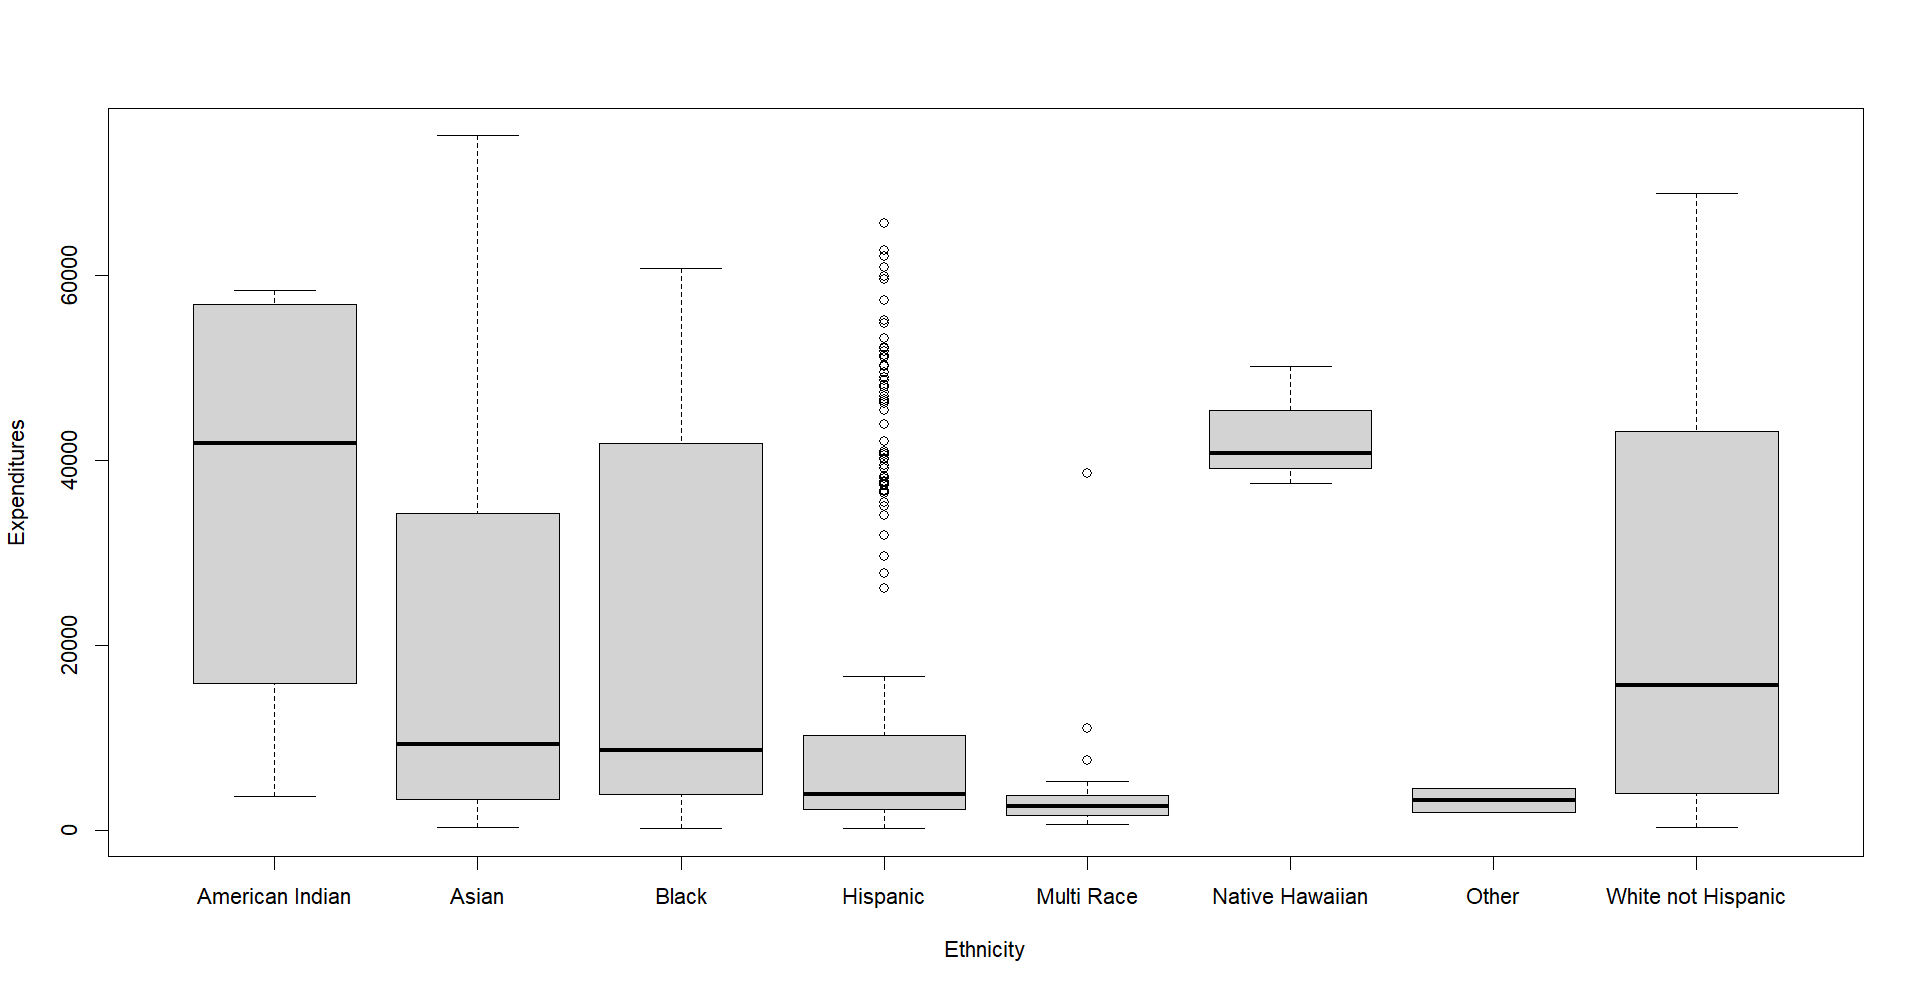
\includegraphics[scale=0.45]{FIG1-Expenditures_Ethnicity-Boxplot-Raw}
		Figure 1: Expenditures by Ethnicity
	\end{center}
	
	This gives an idea of where expenditures are going across all Ethnic groups. To get a greater idea about just the Hispanic and White ethnicities, I subsetted the data and created bar graphs of expenditures for just those two ethnicities.
	\begin{center}
		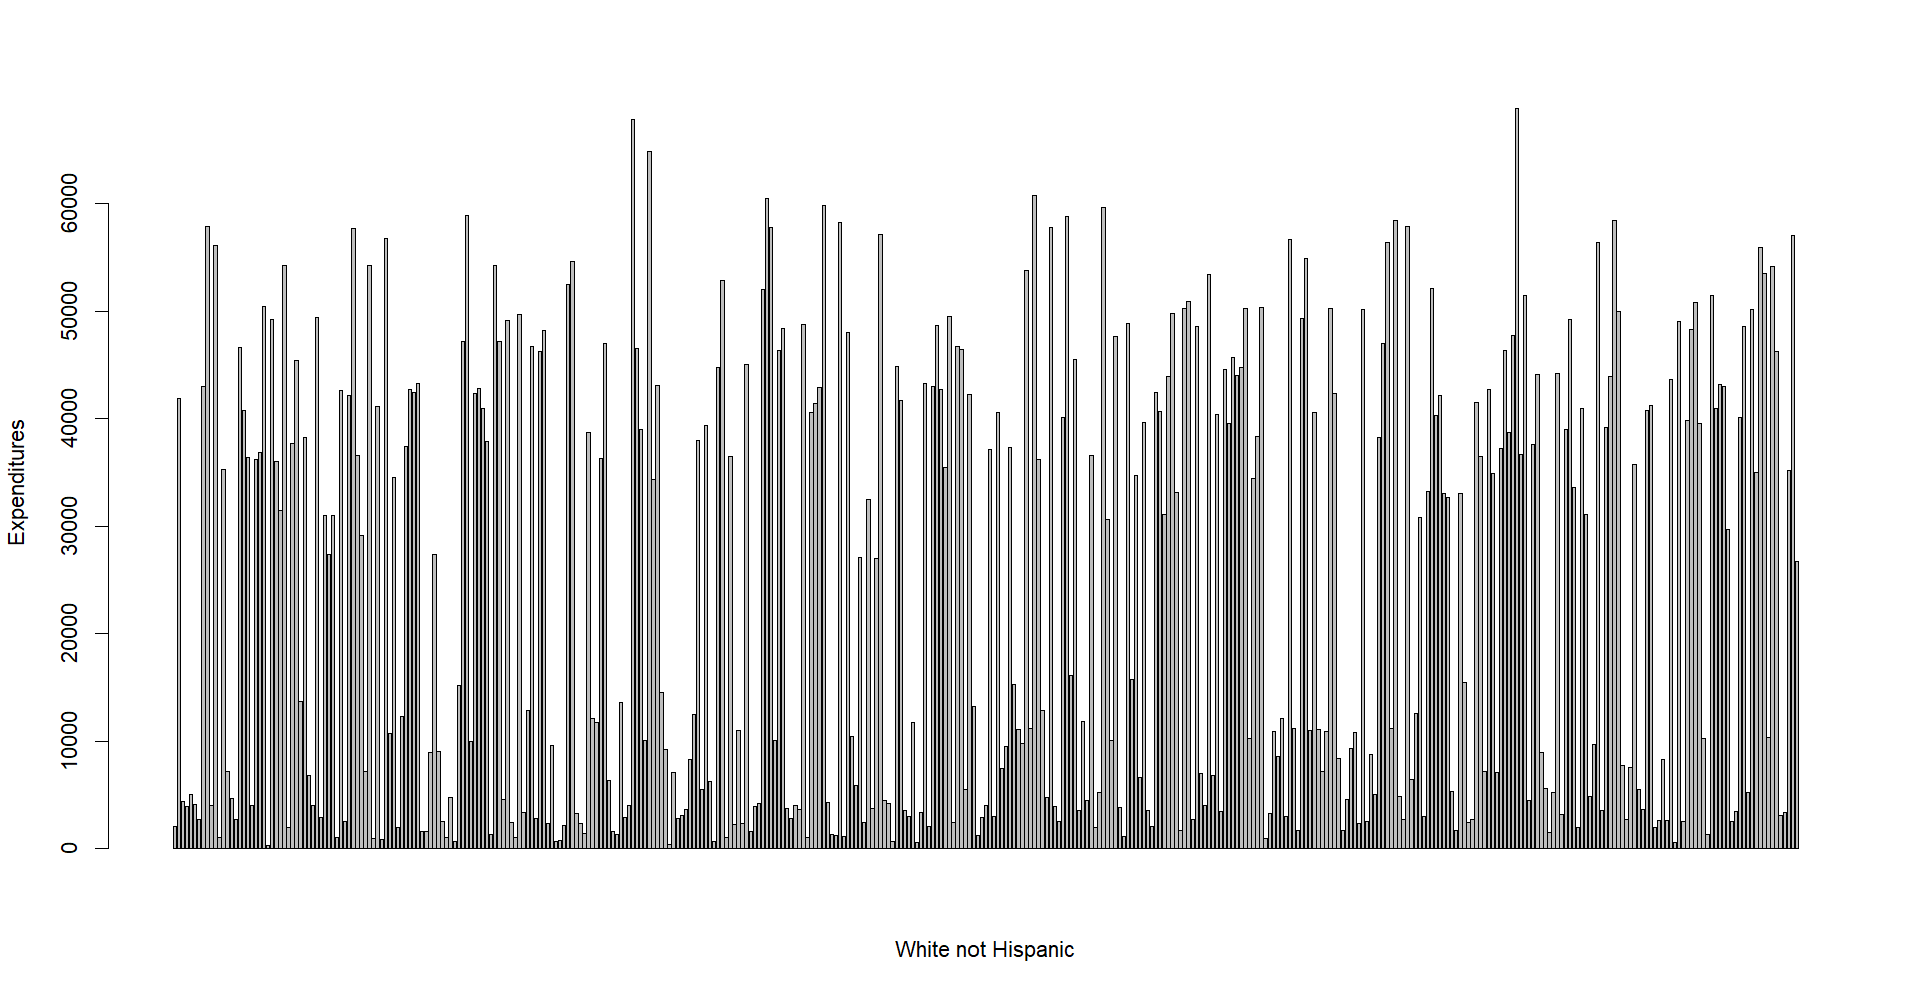
\includegraphics[scale=0.45]{FIG2-Expenditures-Barplot-WhiteNotHispanic}
		Figure 2: Expenditures for White non Hispanics
		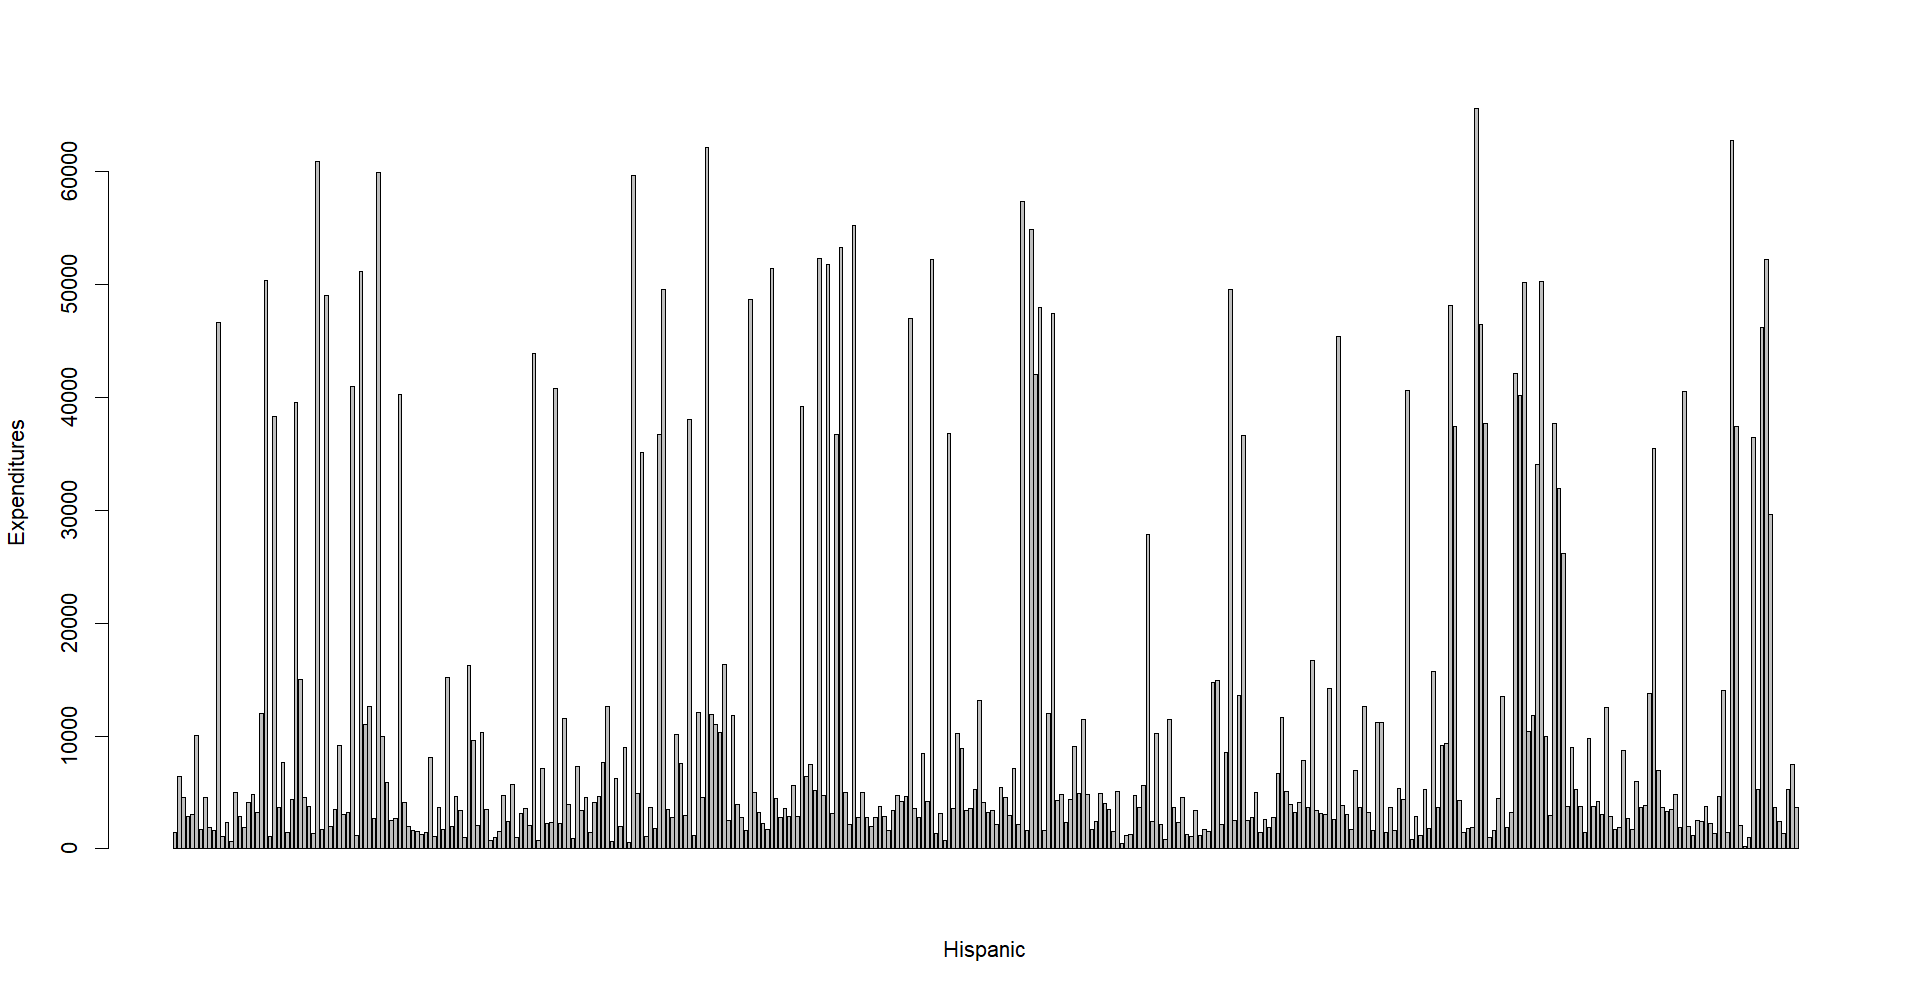
\includegraphics[scale=0.45]{FIG3-Expenditures-Barplot-Hispanic}
		Figure 3: Expenditures for Hispanics
	\end{center}
	These initial results do not look very good for the company comparing these two bar charts and looking at the box plot. The box plot reveals clearly higher average expenditures for White non Hispanics, with their average being much higher than that for Hispanic individuals. Given that the frequency of expenditures looks to be similar for both Hispanics and White non Hispanics, it does appear from these results that there are far larger expenditures being given to White non Hispanics more frequently compared to Hispanics.
	
	\subsection{Expenditures by Ethnicity Subsetted by Age}
	Despite the initial data not looking very good for the company, this is still very broad. To further test if there was any discrimination, I subsetted the data again, this time by age groups, to get more accurate results since different age groups require different amounts of expenditures (Figures 4-9). Based on these figures, especially, when looking at Hispanics and White non Hispanics, there appears to be no major difference in expenditures across the different age groups. The average expenditures tend to be close to each other, and maximum expenditures are usually only within a few thousand of each other at most, some being only within hundreds of each other.
	
	\subsection{Expenditures by Gender Subsetted by Age}
	A very common vector of discrimination is based on gender. Given that I'm already looking at discrimination based on ethnicity, I also checked whether or not there could be a basis for discimination based on gender. To do that, I once again subsetted the data, this time based on age. I then subsetted the gender data by the same age groups as before, creating bar graphs for each gender and age group combination (Figures 10-21). Based on the bar charts, the expenditures for the different age groups are very similar between males and females of the same age groups. So far, I do not see any source of discrimination by gender.
	
	\subsection{Expenditures by Gender Subsetted by Ethnicity}
	To run further analyses about potential gender-based discrimination, I also subsetted the gender data by ethnicity, generating bar graphs for each gender and ethnicity combination (Figures 22-37). Ignoring the ones where there are only at most 3 results, since there isn't much of anything to analyze on these, it really does vary which gender is getting more expenditures for each ethnicity. In generally some may be getting far larger maximum expenditures, but it's not clearly steered towards one gender or another. This leads to me to believe that there is not discrimination based on gender.
	
	\section{Results}
	\subsection{Discrimination against Hispanics}
	The initial results when just looking at raw data of the expenditures for each ethnicity, and more specifically when looking at the expenditures for just White non Hispanics and Hispanics, are not great. There appears to be far larger expenditures going to White non Hispanic individuals compared to Hispanic individuals when looking at the bar charts for each ethnicity. Additionally, when looking at the box plot of all ethnicities, the average expenditure for White non Hispanic individuals are much higher than for Hispanic individuals.
	
	However, when you break down the data further based on age, a lot more gets revealed. In general, different age groups require different amounts of expenditures, so looking at the different age groups will paint much clearer pictures. When analyzing these box plots, the expenditures are much more in line with each other within the different age groups. The averages are much closer together, and there's not generally a huge difference in maximum and minimum expenditures across the different age groups. So in the end, there does not seem to be any discrimination against Hispanics compared to White non Hispanics currently happening at the California DDS.
	
	\subsection{Discrimination based on Gender}
	Identifying discrimination towards gender is another thing I tested for while I was already testing for the ethnicity-based discrimination. By subsetting the raw data by gender and age group, there is no apparent discrimination based on gender. The expenditures were reasonably different enough to where it just appears that different people in each age group may require different amounts of expenditures, which may result in slightly higher or lower expenditures for different genders.
	
	The gender data was then subsetted by ethnicity, and while there might have been some stark differences in expenditure sizes, it once again wasn't enough to be alarming. Therefore, there does not seem to be any discrimination, as of right now, based on gender.
	
	\section{Summary and Conclusions}
	Based on the raw data, it's plausible that there could be some discrimination against Hispanics compared to White non-Hispanics. However, raw data rarely tells the full story. Subsetting the data, as we did by age groups, can shed a lot of light, as different age groups may require different amounts of expenditures. By subsetting the data, a much clearer picture is given to us, and we can make a more informed decision. The same is true for checking data regarding gender-based discrimination. It would not have been worthwhile to look at raw data of just males and just females of all ages and ethnicities. By subsetting the data, we can ensure a full picture, and confidently say the California Department of Development Service is not experience any discrimination against Hispanics compared to White Non-Hispanics, or based on gender.
	
	\newpage
	\section{Appendices}
	\subsection{Figures}
	\begin{center}
		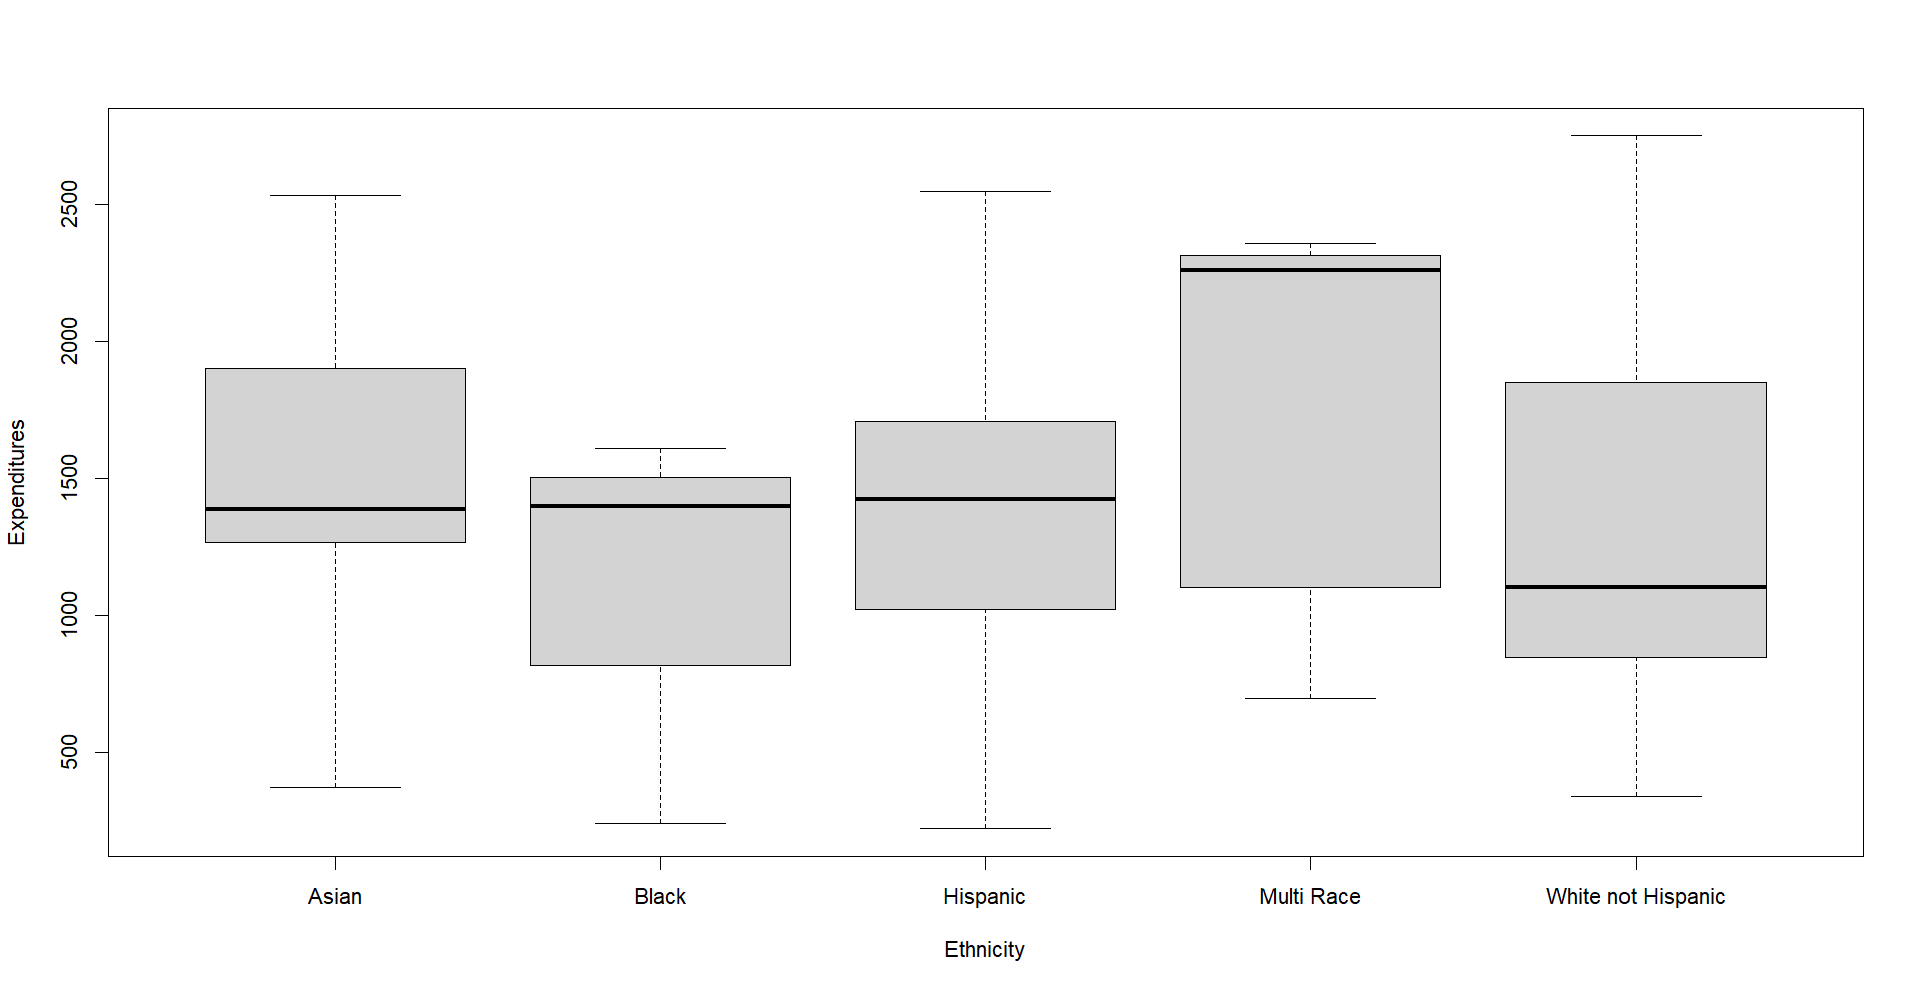
\includegraphics[scale=0.45]{FIG4-Expenditures_Ethnicity-Boxplot-Age_0-5}
		Figure 4: Expenditures by Ethnicity for Ages 0-5
		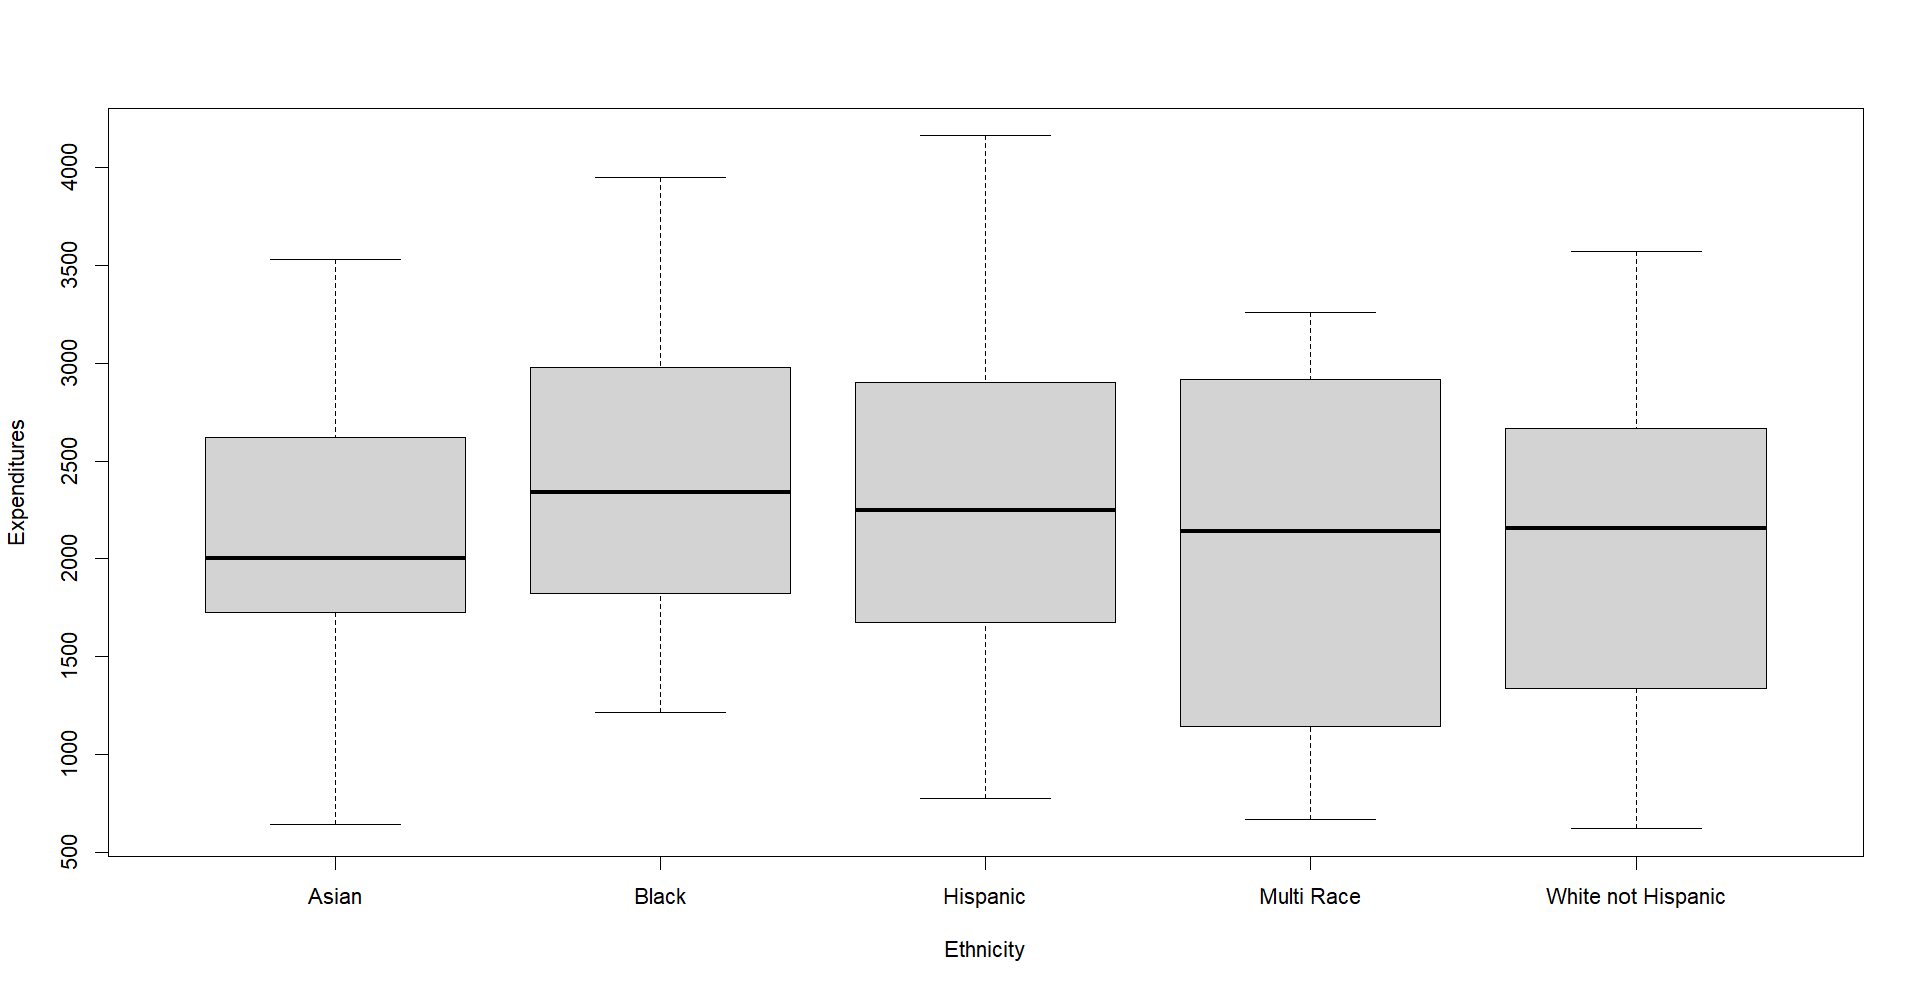
\includegraphics[scale=0.45]{FIG5-Expenditures_Ethnicity-Boxplot-Age_6-12}
		Figure 5: Expenditures by Ethnicity for Ages 6-12
		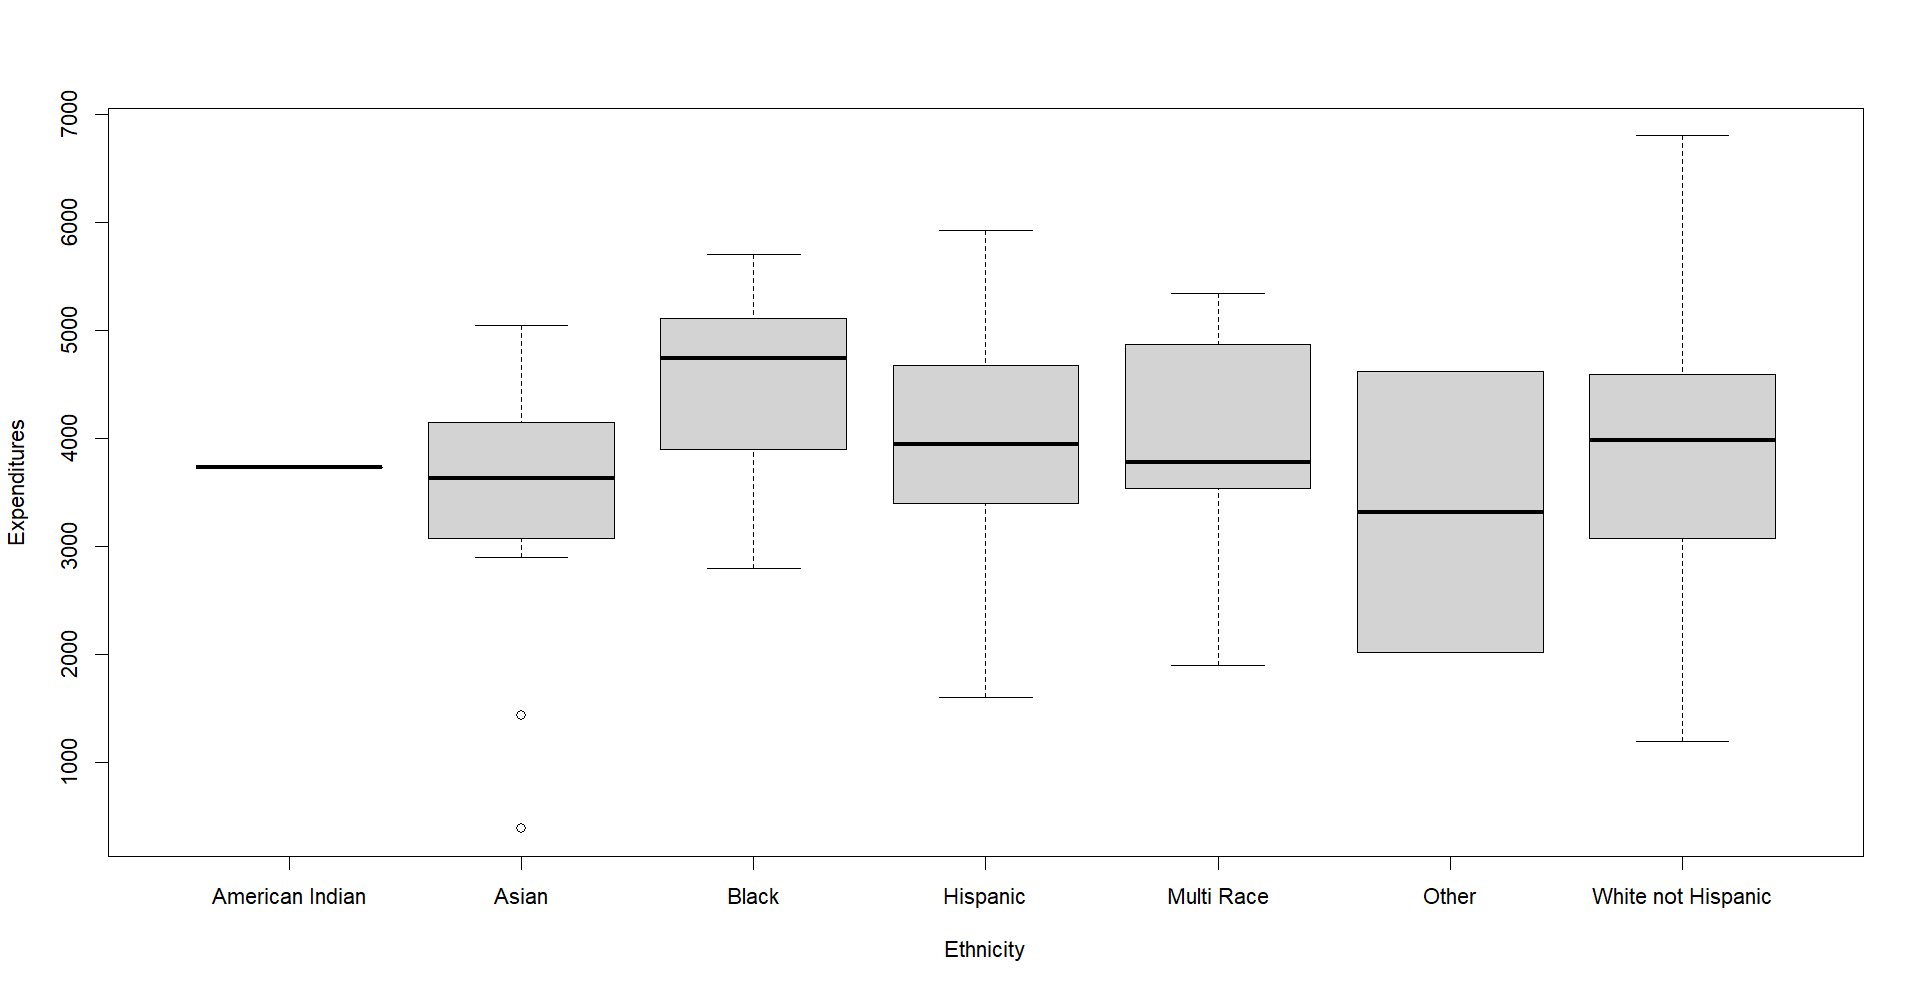
\includegraphics[scale=0.45]{FIG6-Expenditures_Ethnicity-Boxplot-Age_13-17}
		Figure 6: Expenditures by Ethnicity for Ages 13-17
		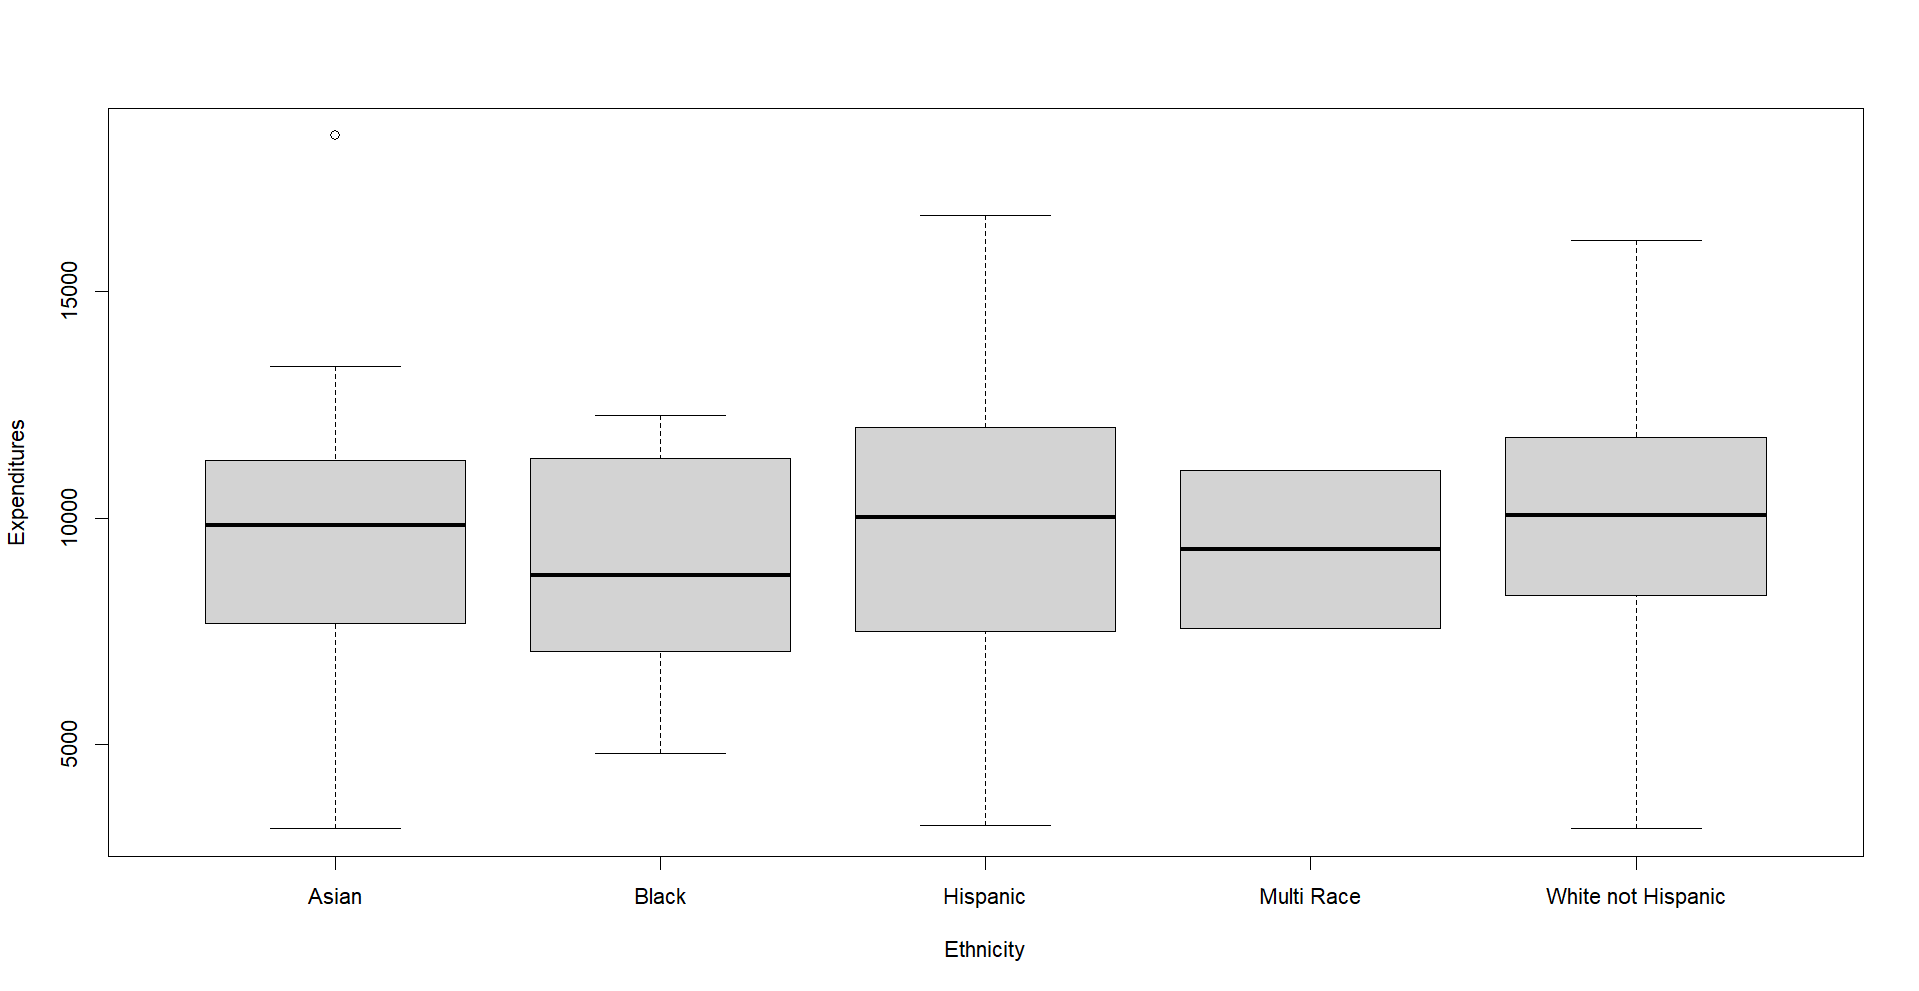
\includegraphics[scale=0.45]{FIG7-Expenditures_Ethnicity-Boxplot-Age_18-21}
		Figure 7: Expenditures by Ethnicity for Ages 18-21
		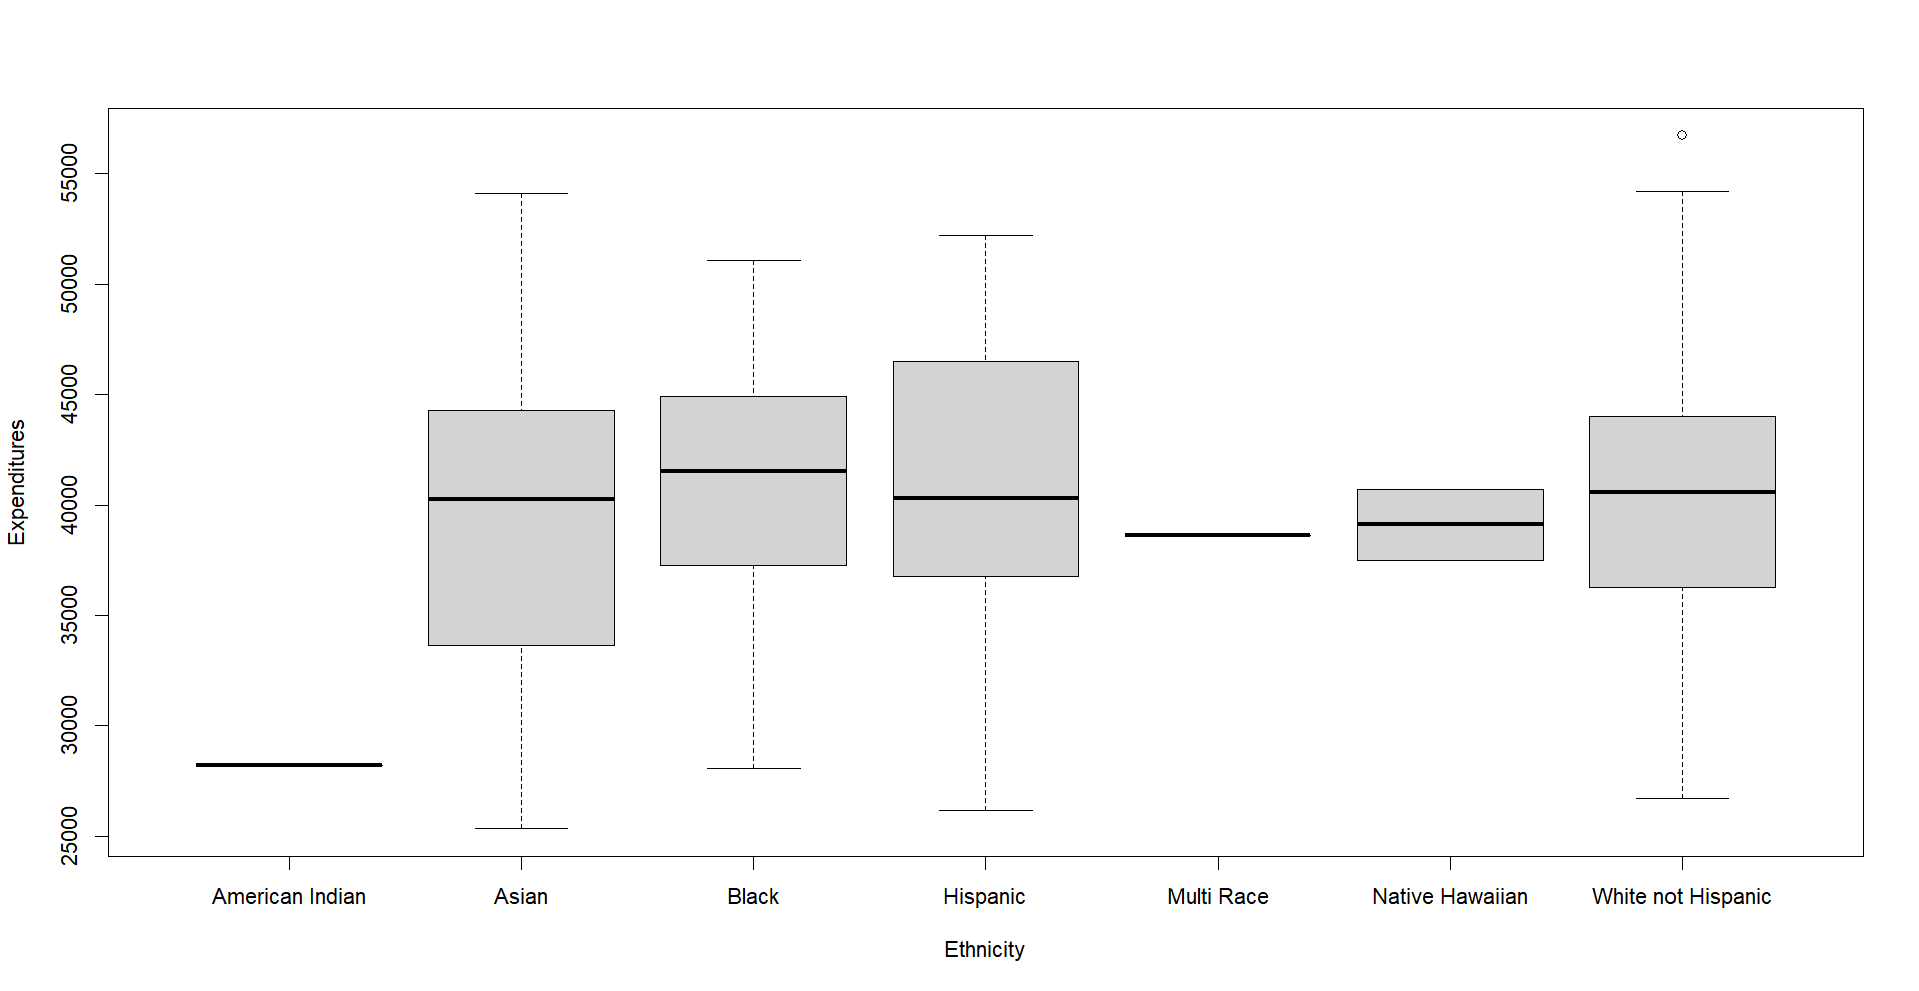
\includegraphics[scale=0.45]{FIG8-Expenditures_Ethnicity-Boxplot-Age_22-50}
		Figure 8: Expenditures by Ethnicity for Ages 22-50
		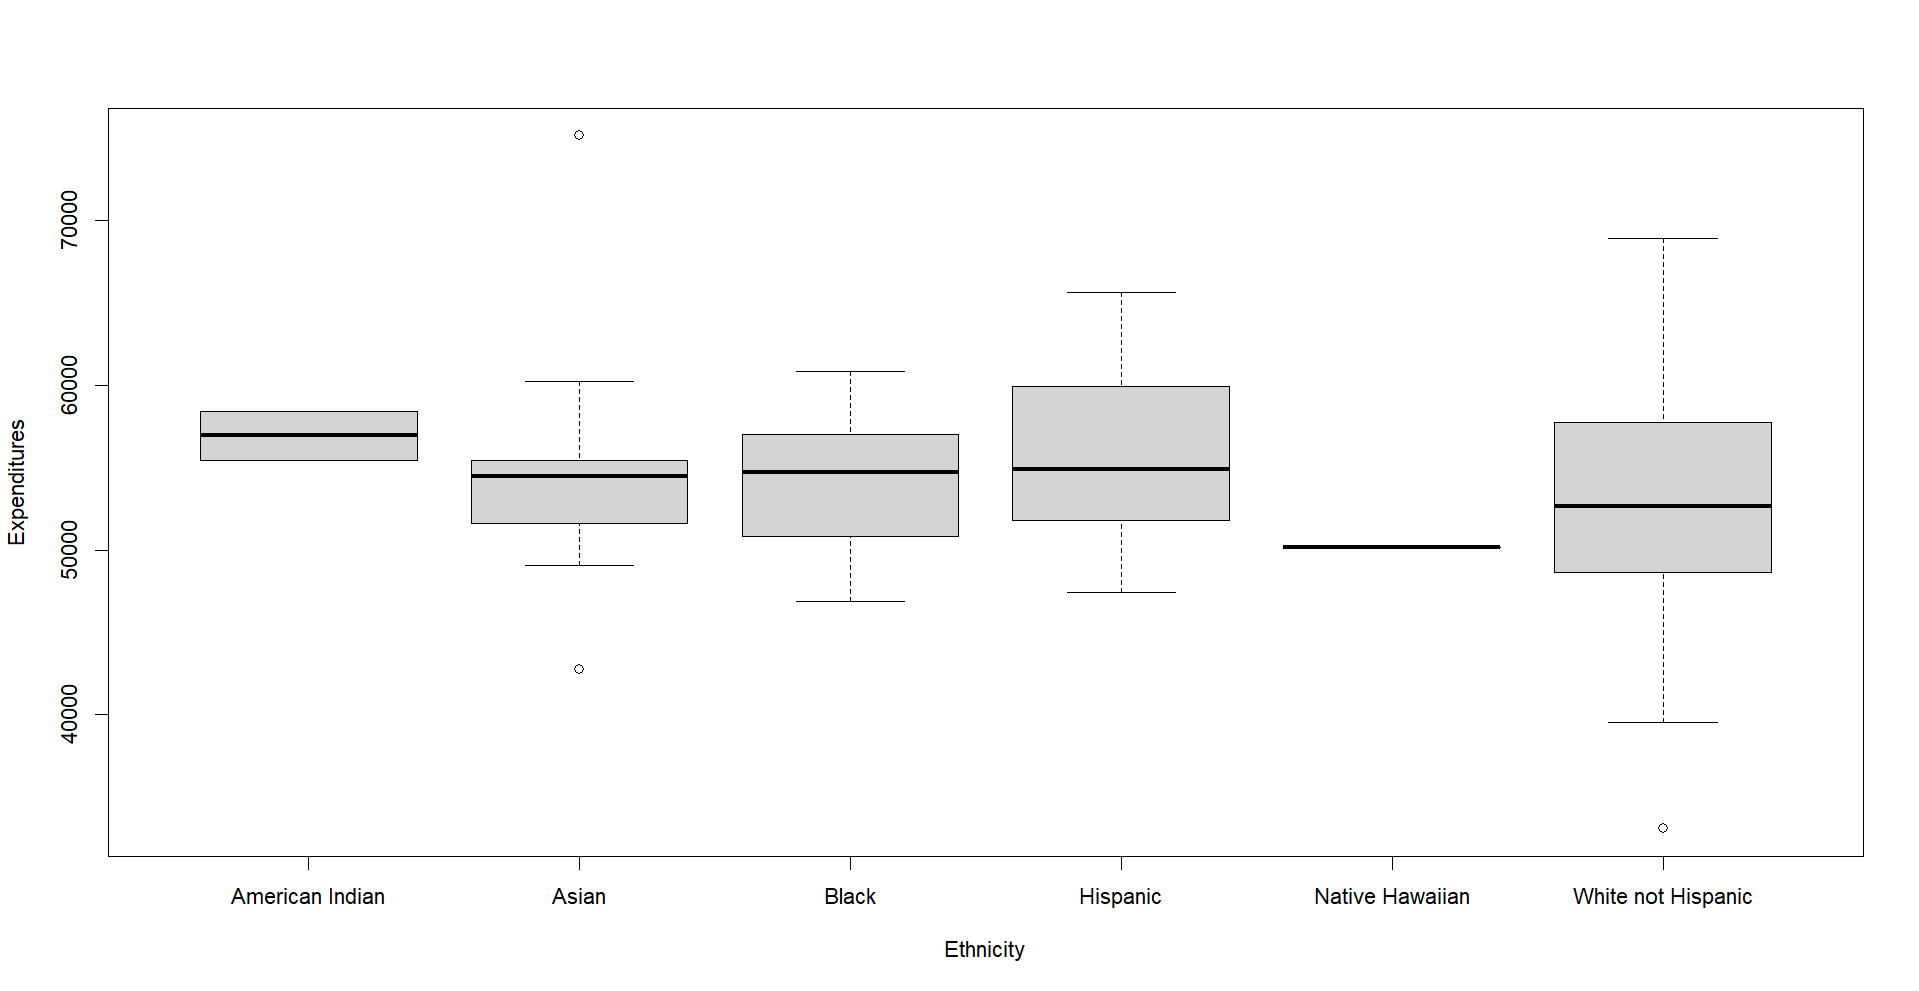
\includegraphics[scale=0.45]{FIG9-Expenditures_Ethnicity-Boxplot-Age_Over51}
		Figure 9: Expenditures by Ethnicity for Ages 51+
		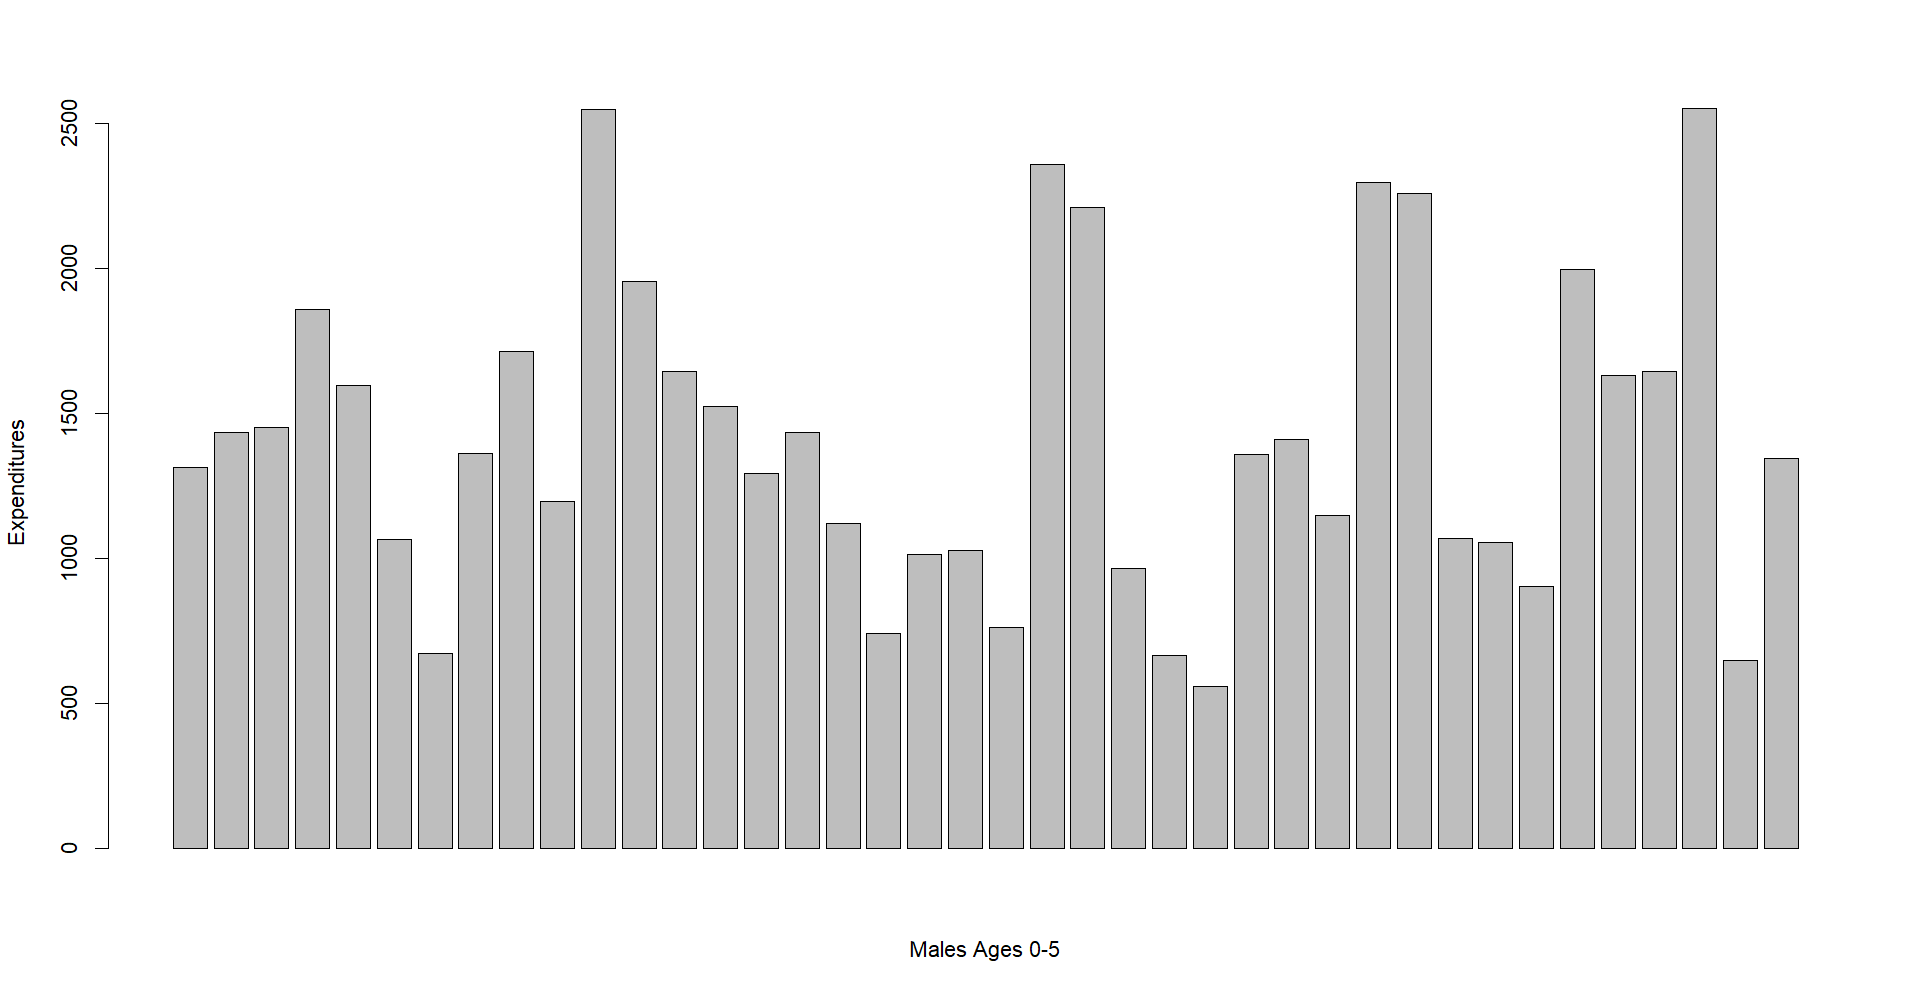
\includegraphics[scale=0.45]{FIG10-Expenditures-Barplot-Male_0-5}
		Figure 10: Expenditures for Males Age 0-5
		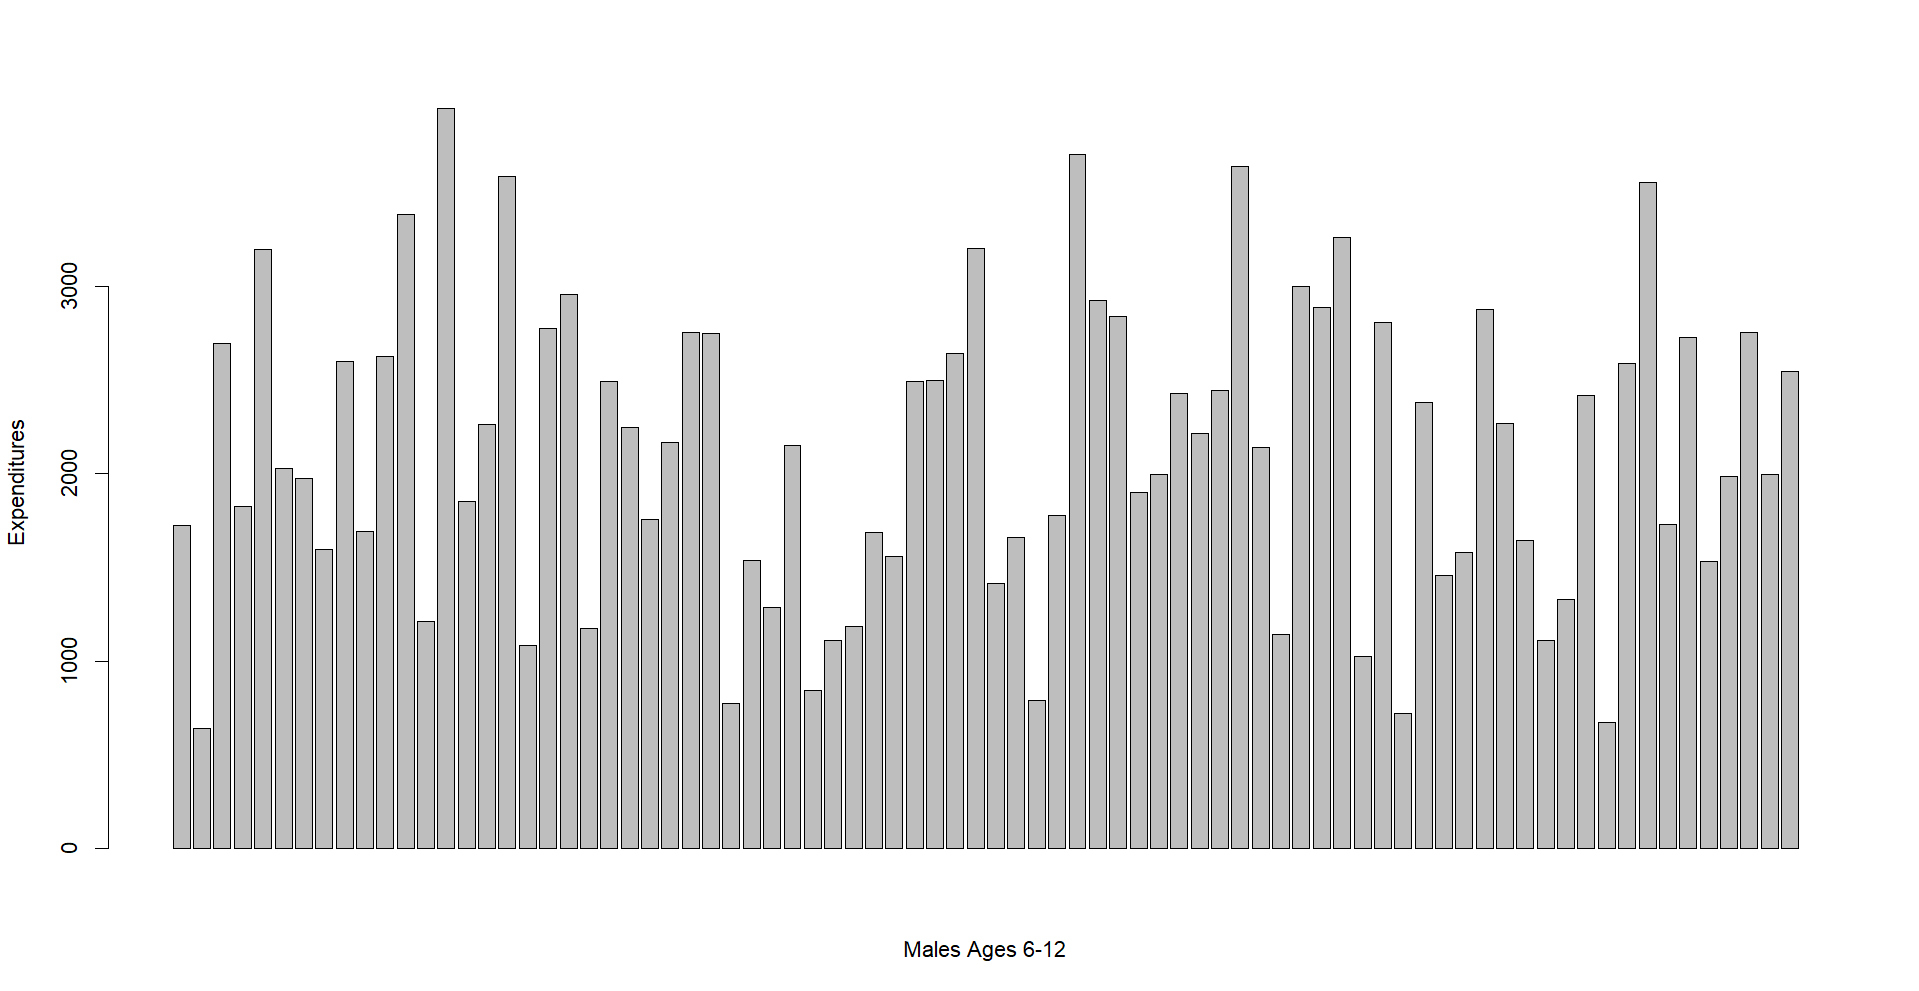
\includegraphics[scale=0.45]{FIG11-Expenditures-Barplot-Male_6-12}
		Figure 11: Expenditures for Males Age 6-12
		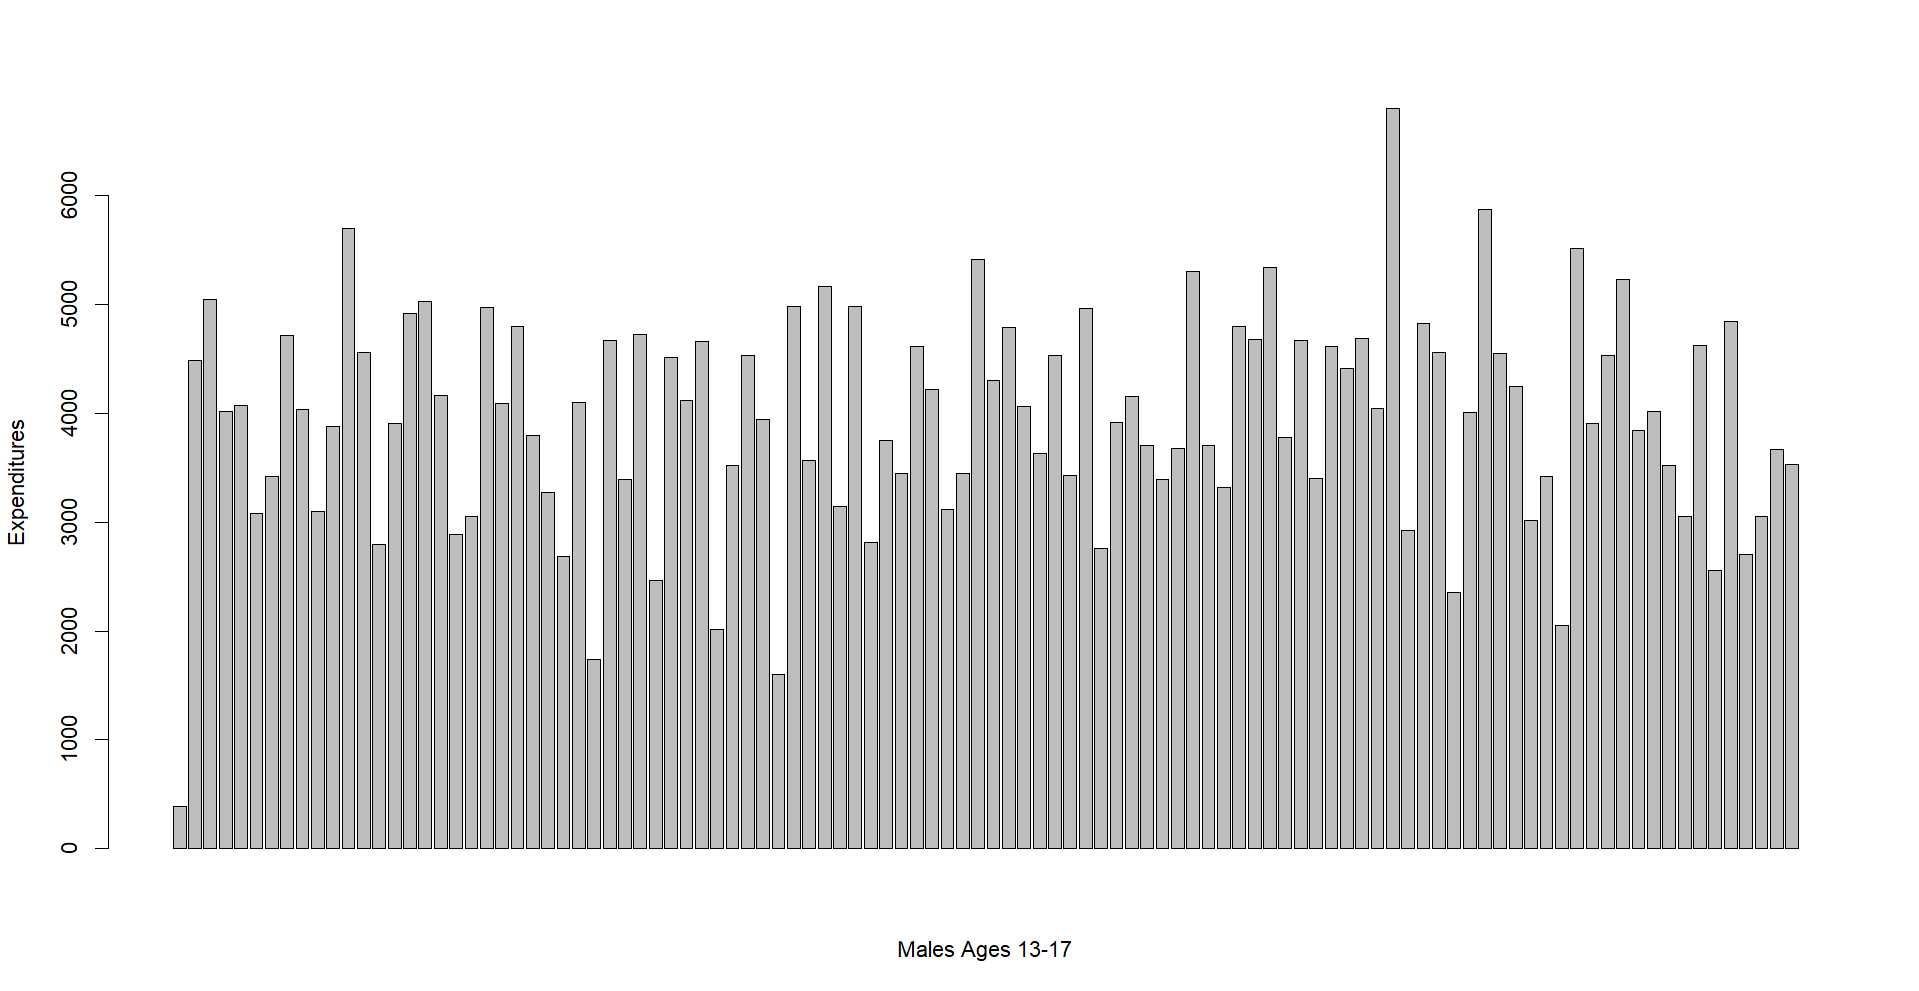
\includegraphics[scale=0.45]{FIG12-Expenditures-Barplot-Male_13-17}
		Figure 12: Expenditures for Males Age 13-17
		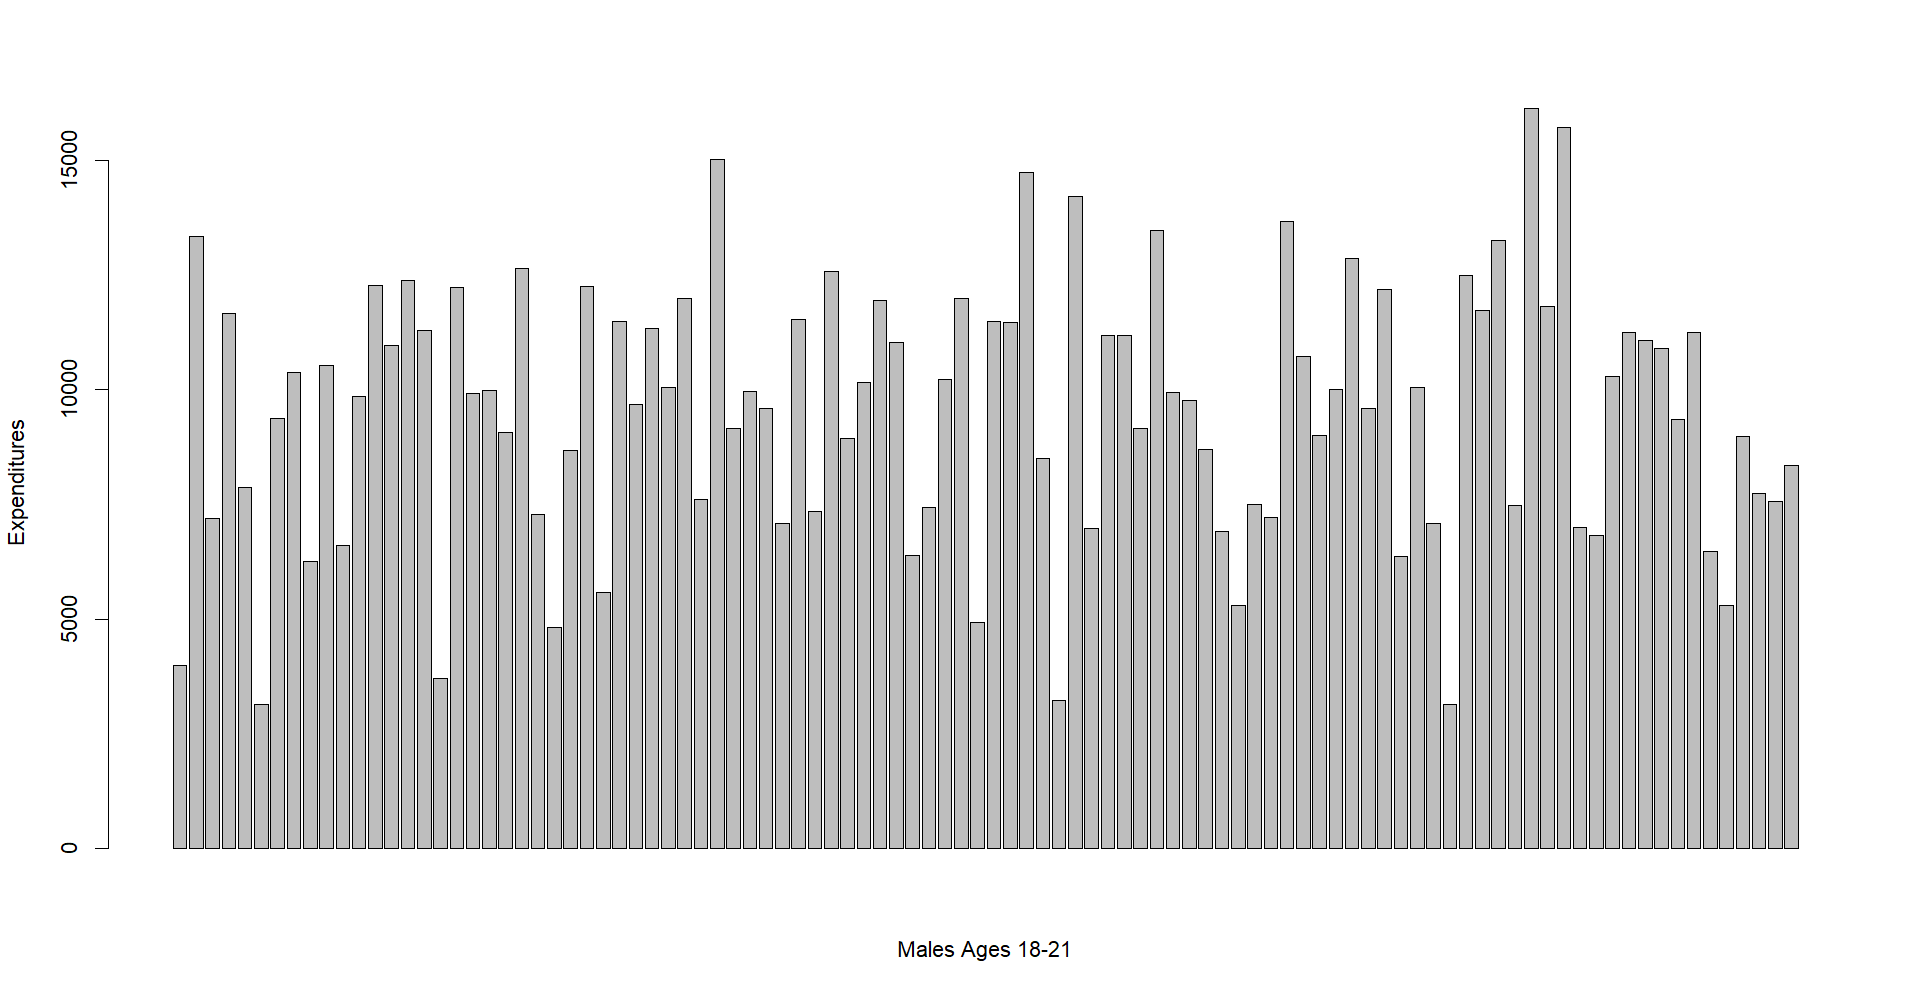
\includegraphics[scale=0.45]{FIG13-Expenditures-Barplot-Male_18-21}
		Figure 13: Expenditures for Males Age 18-21
		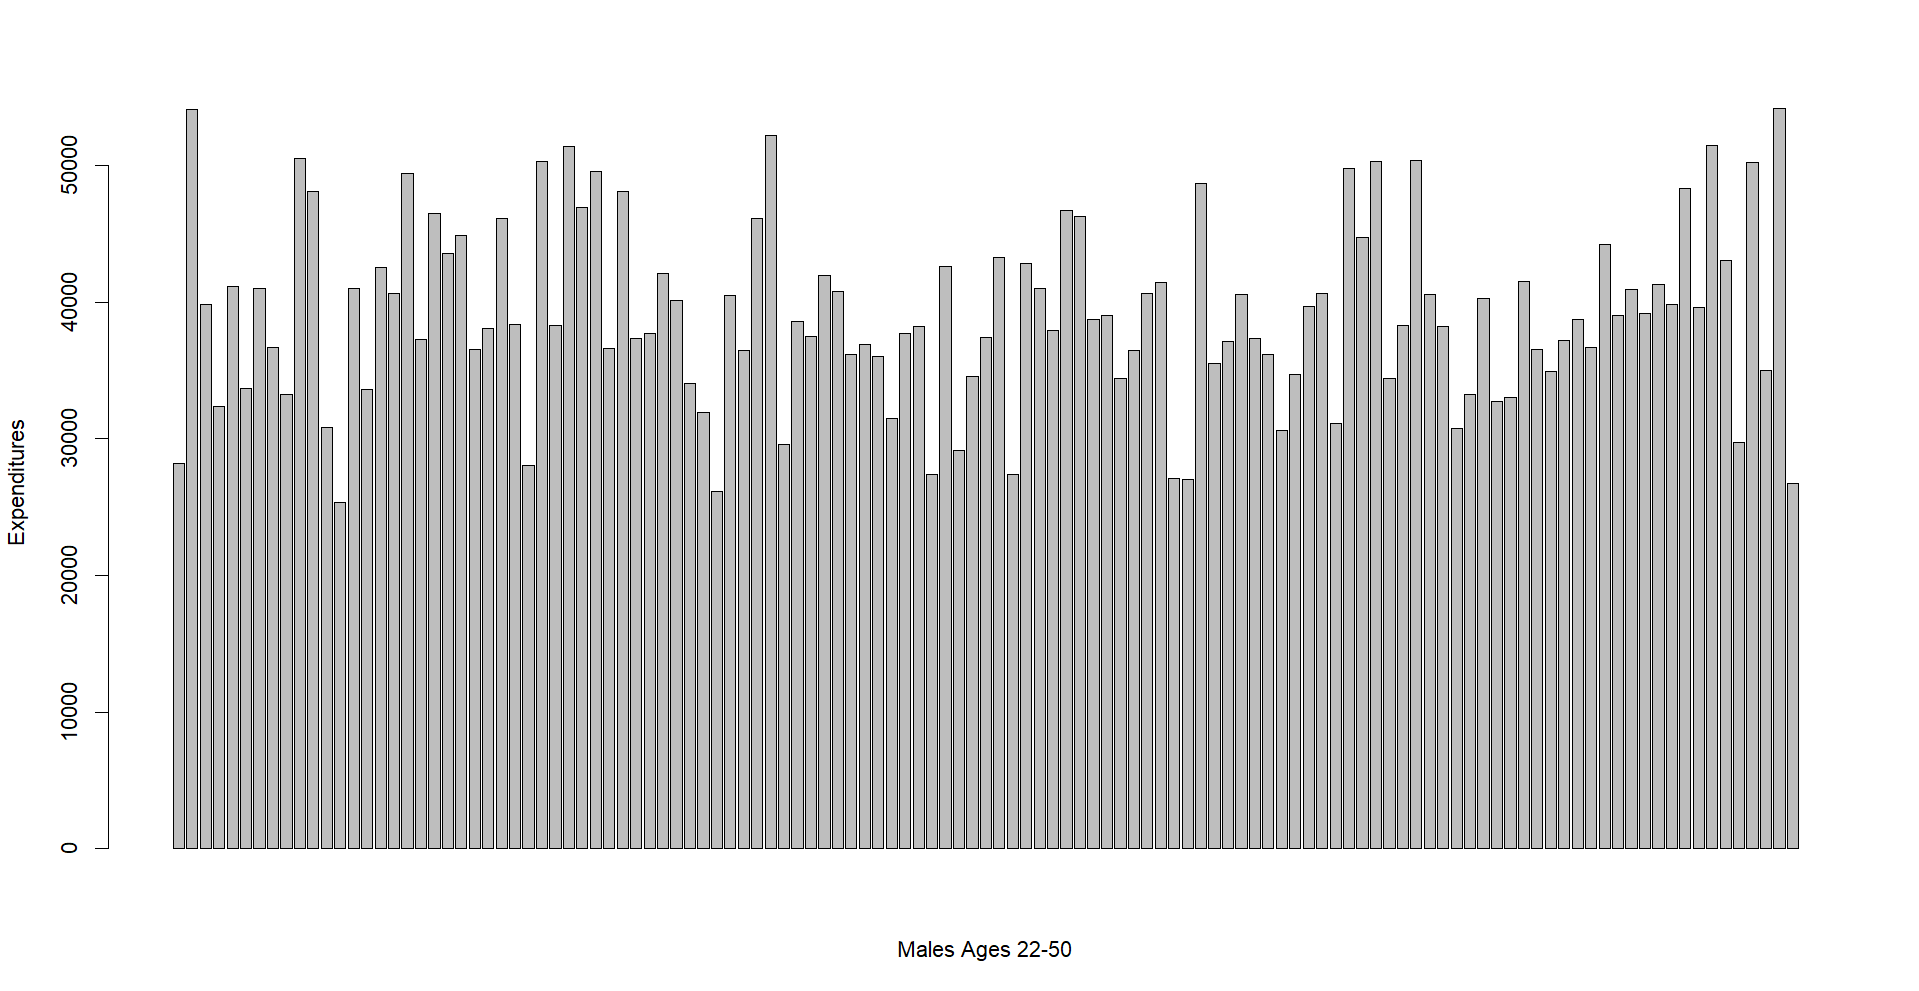
\includegraphics[scale=0.45]{FIG14-Expenditures-Barplot-Male_22-50}
		Figure 14: Expenditures for Males Age 22-50
		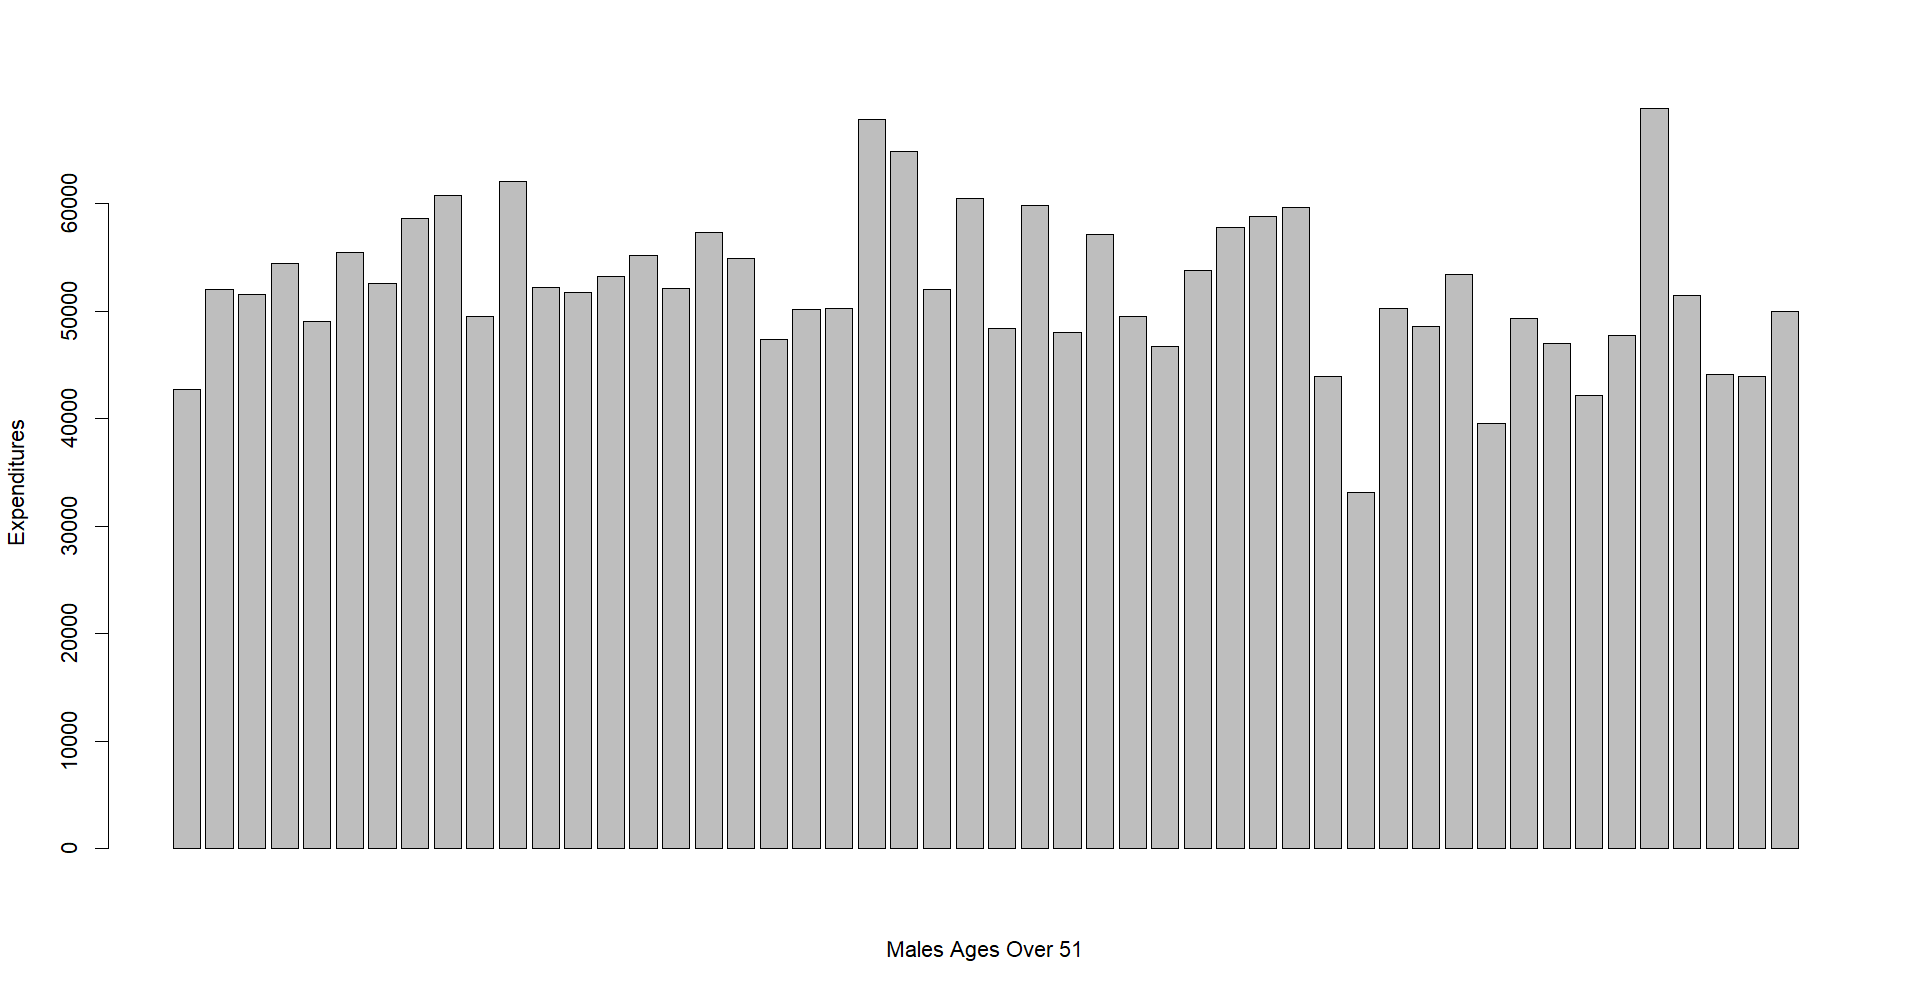
\includegraphics[scale=0.45]{FIG15-Expenditures-Barplot-Male_Over51}
		Figure 15: Expenditures for Males Age Over 51
		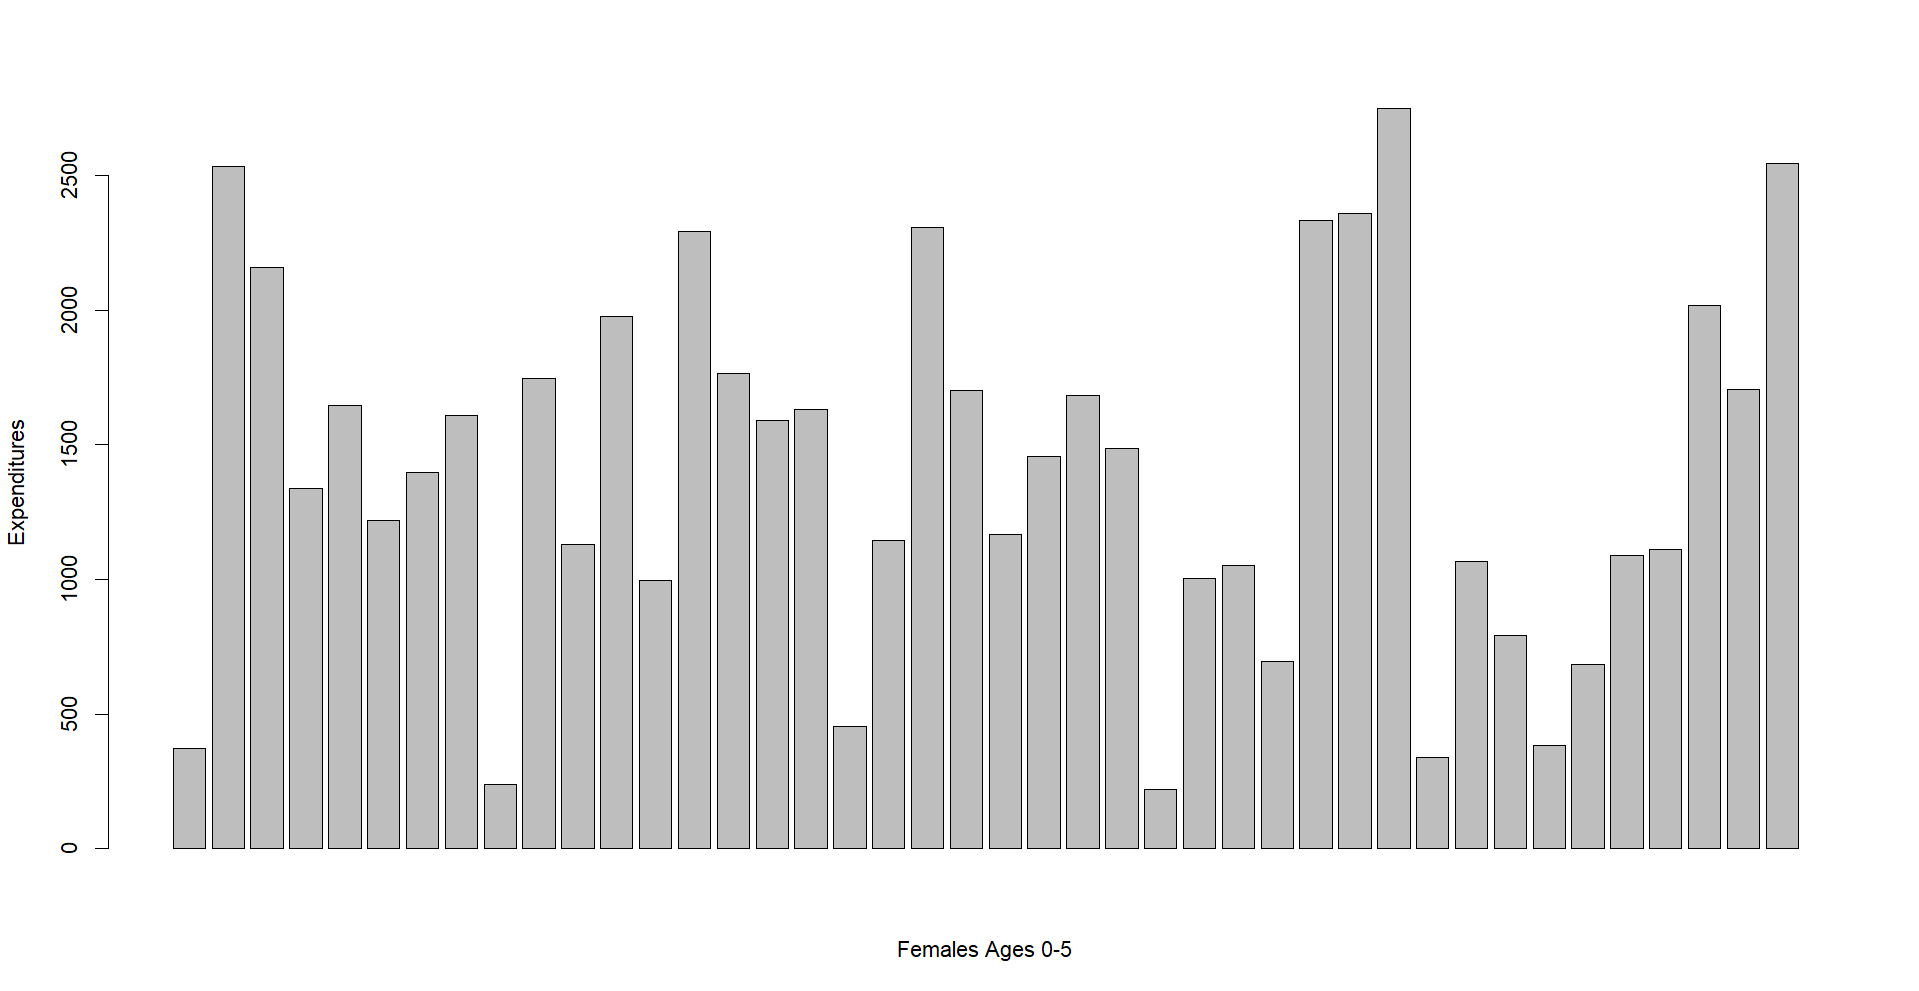
\includegraphics[scale=0.45]{FIG16-Expenditures-Barplot-Female_0-5}
		Figure 16: Expenditures for Females Age 0-5
		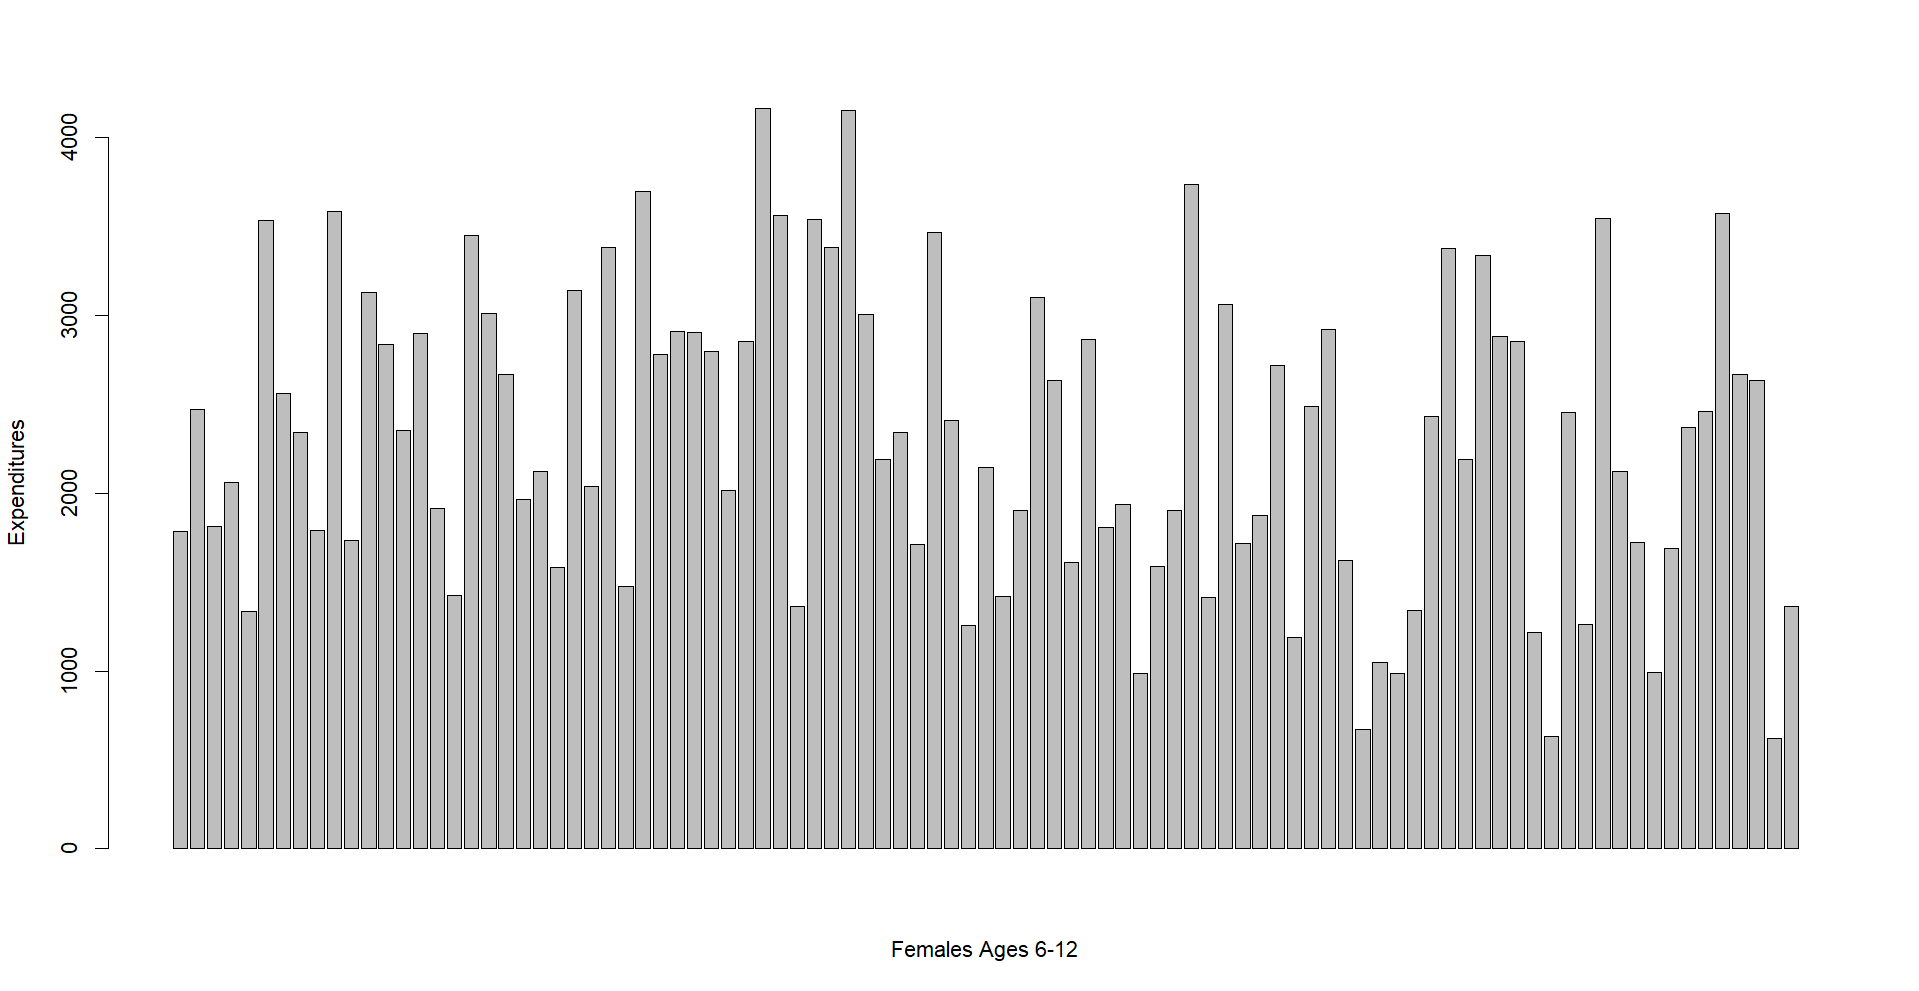
\includegraphics[scale=0.45]{FIG17-Expenditures-Barplot-Female_6-12}
		Figure 17: Expenditures for Females Age 6-12
		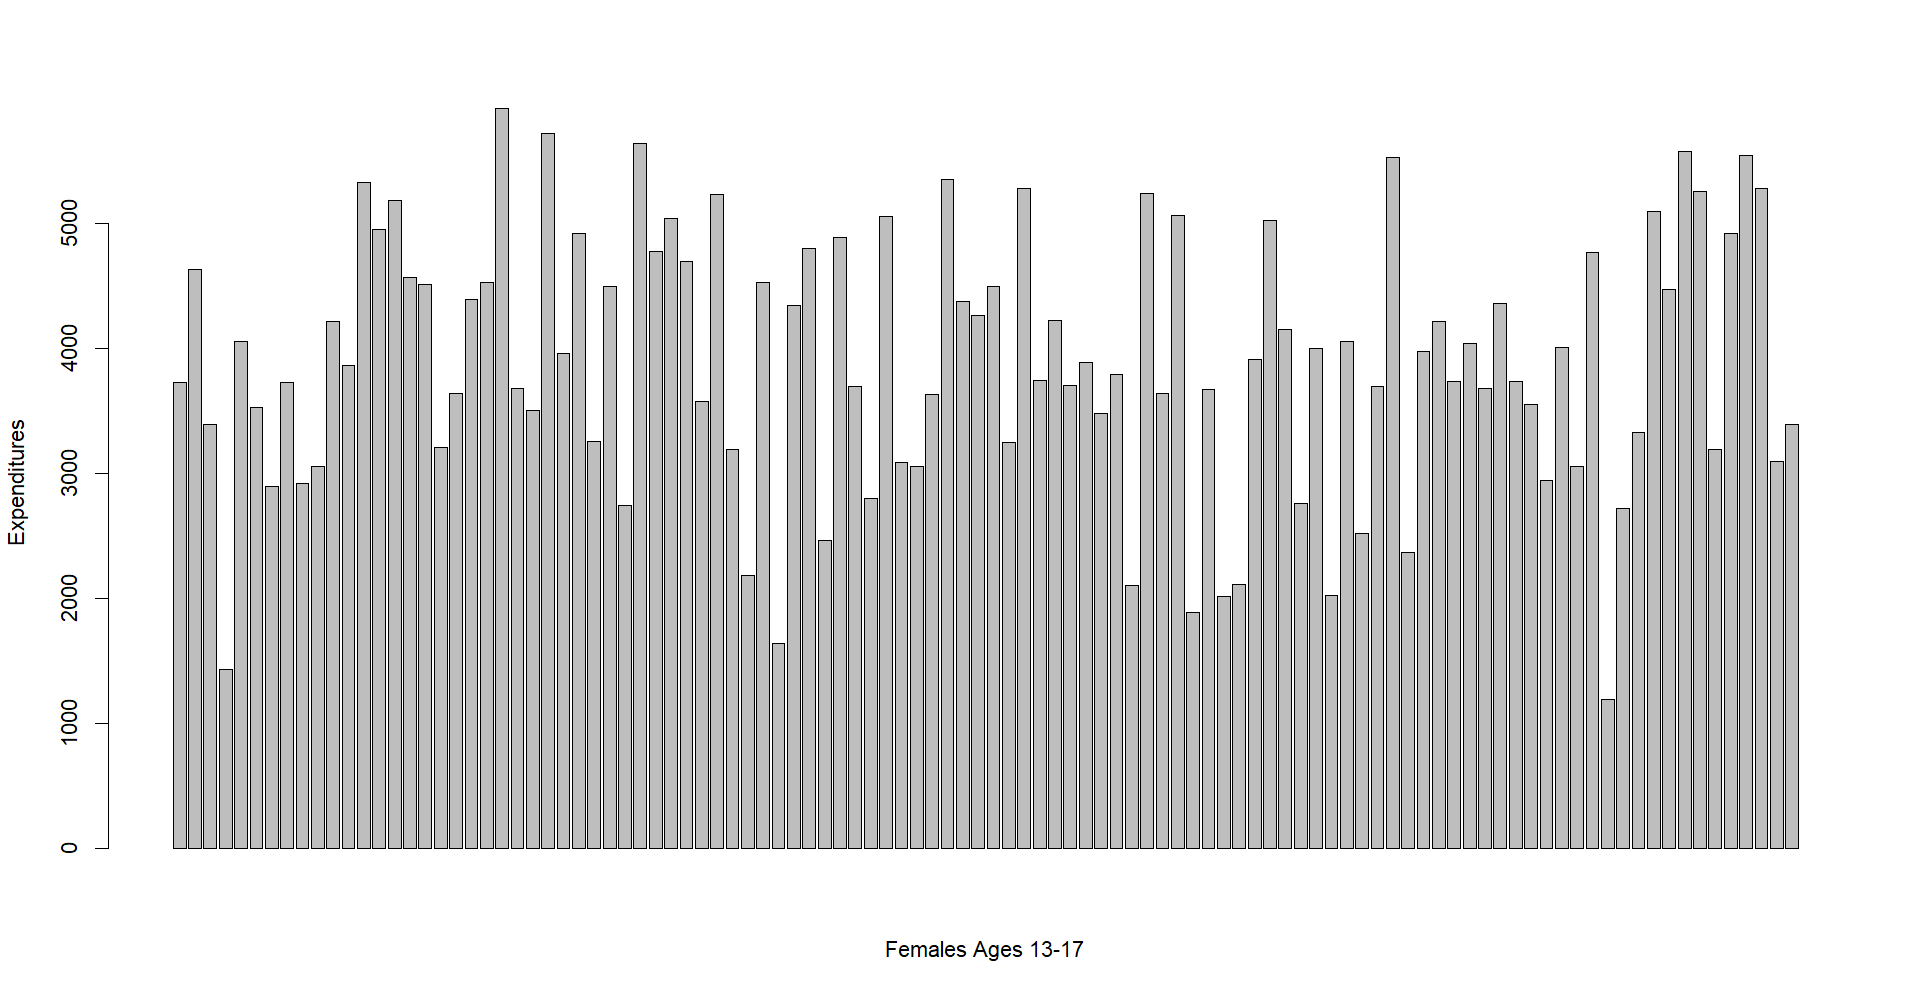
\includegraphics[scale=0.45]{FIG18-Expenditures-Barplot-Female_13-17}
		Figure 18: Expenditures for Females Age 13-17
		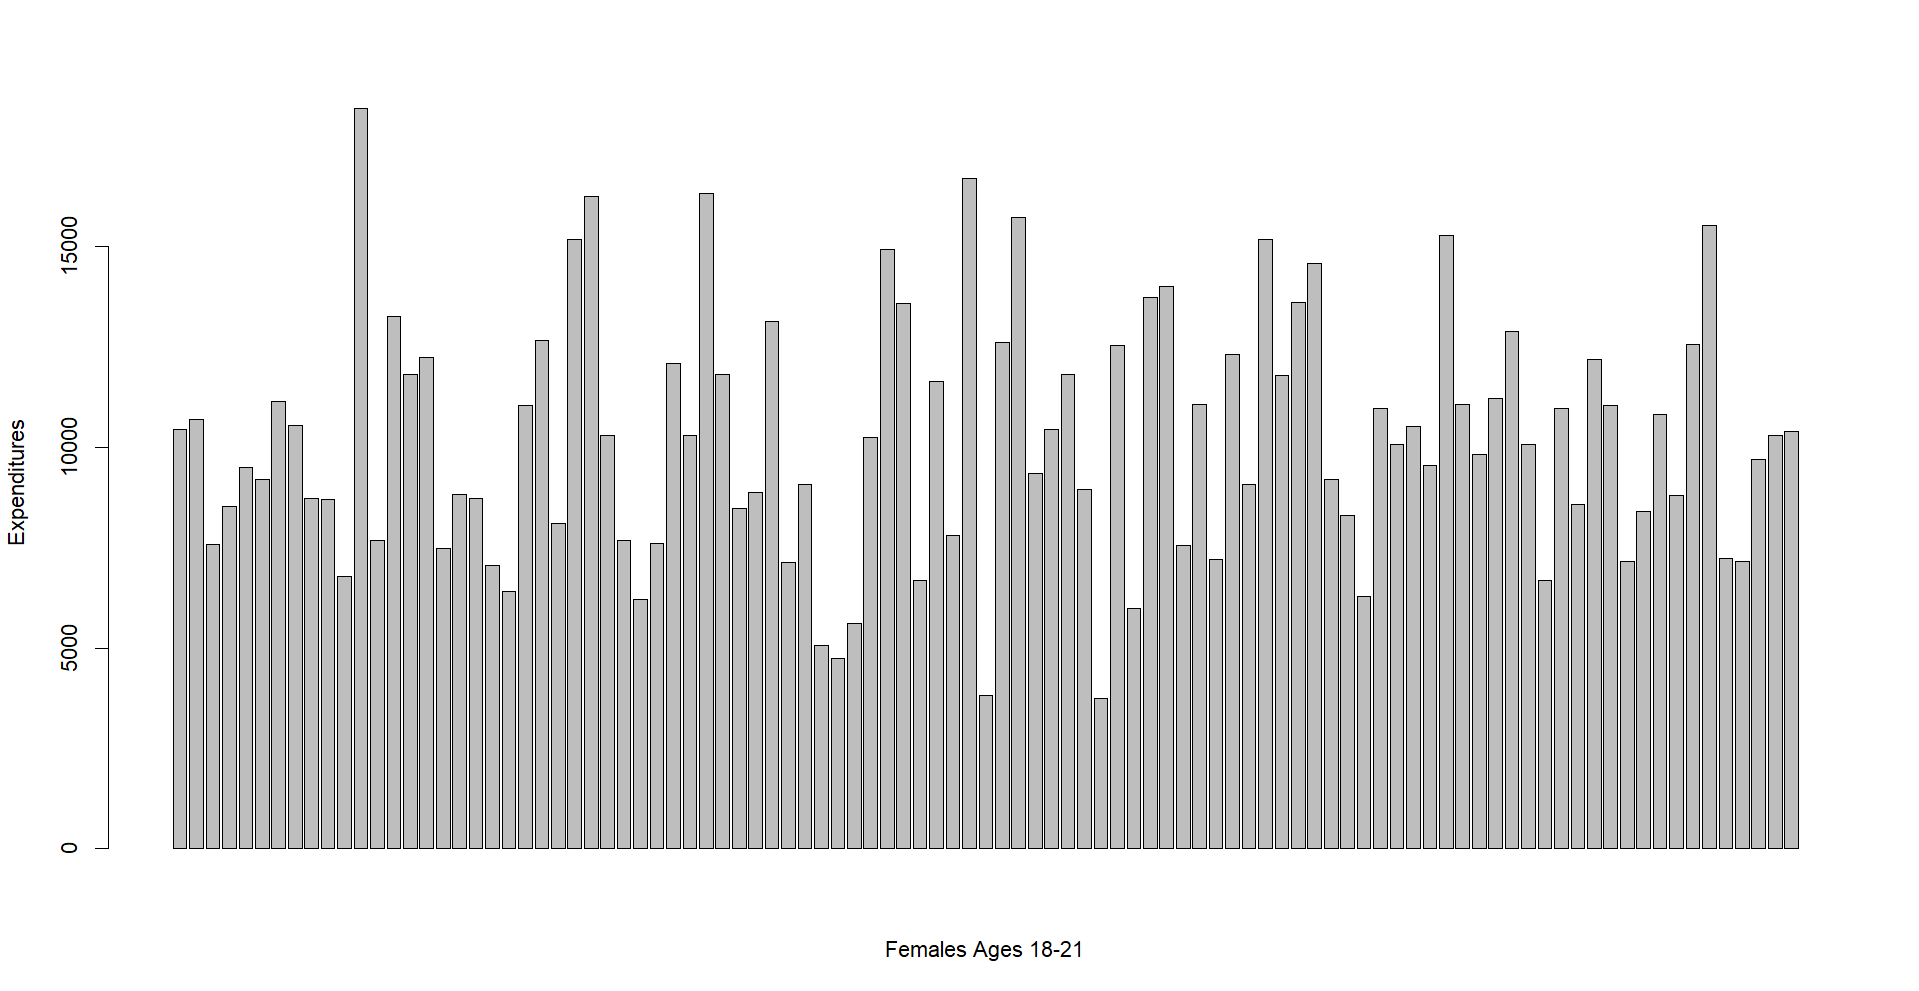
\includegraphics[scale=0.45]{FIG19-Expenditures-Barplot-Female_18-21}
		Figure 19: Expenditures for Females Age 18-21
		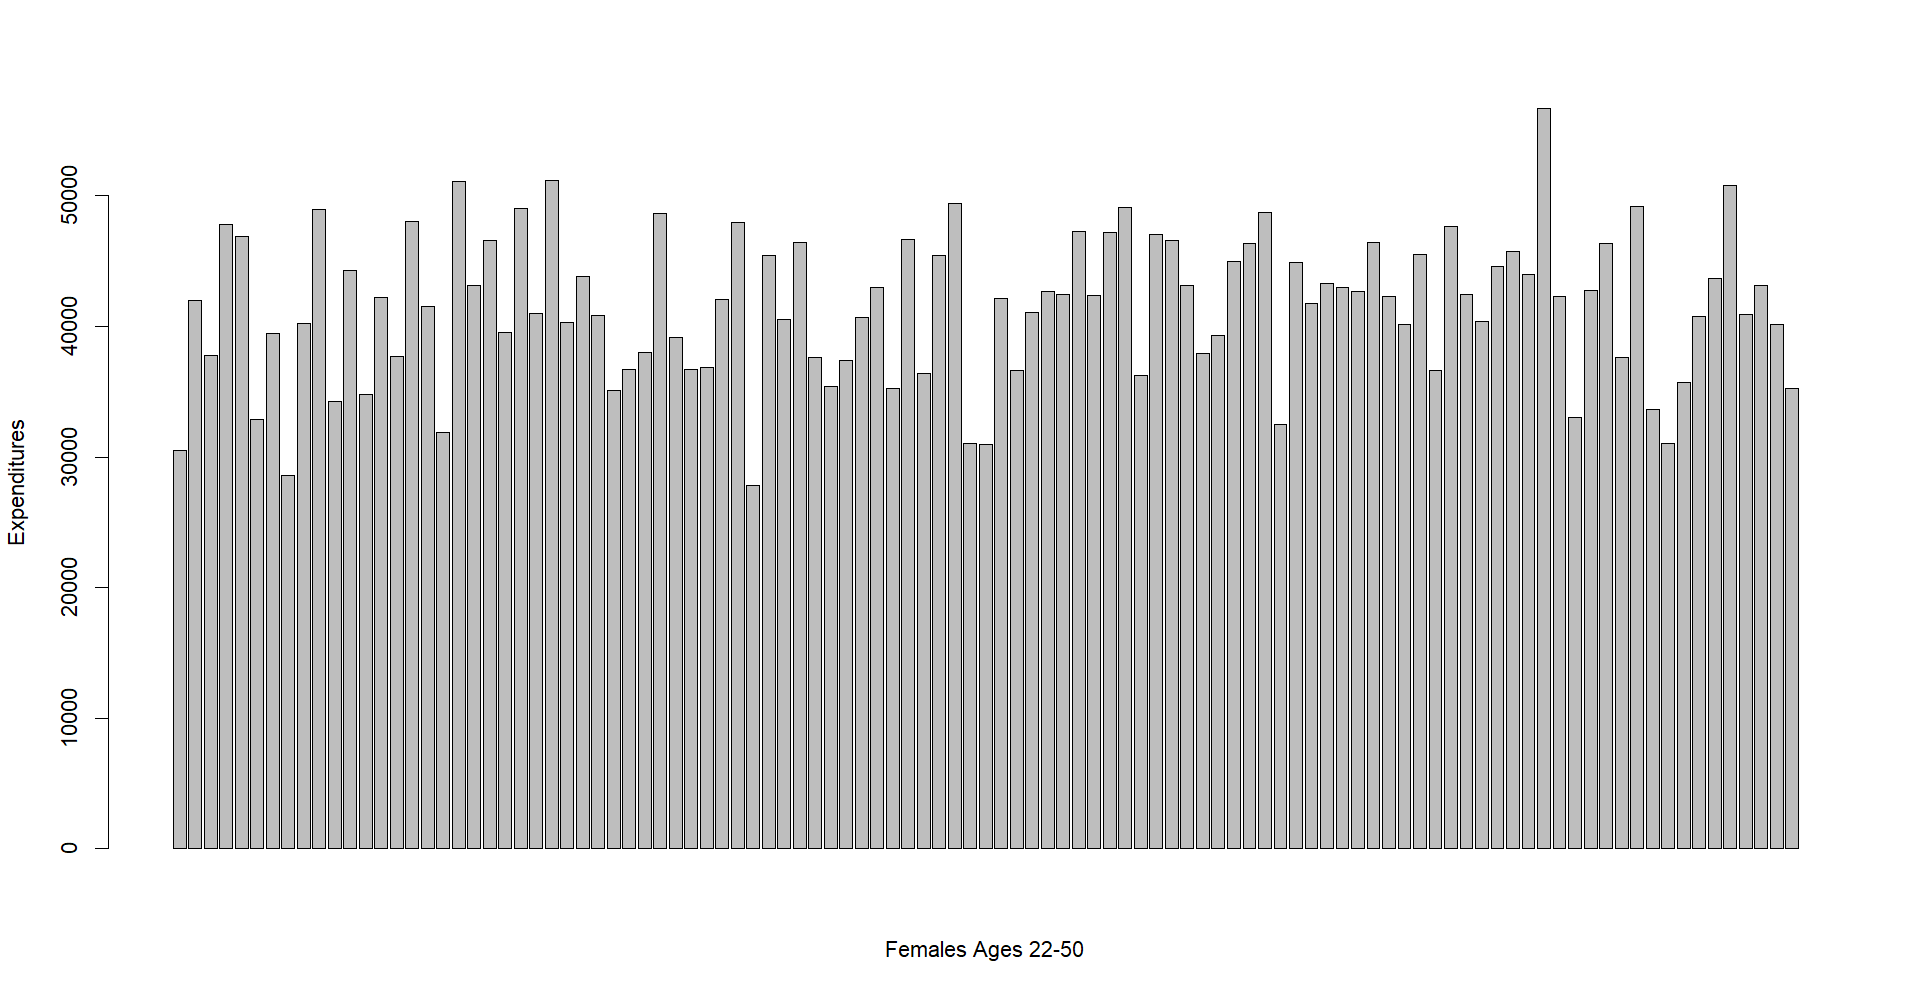
\includegraphics[scale=0.45]{FIG20-Expenditures-Barplot-Female_22-50}
		Figure 20: Expenditures for Females Age 22-50
		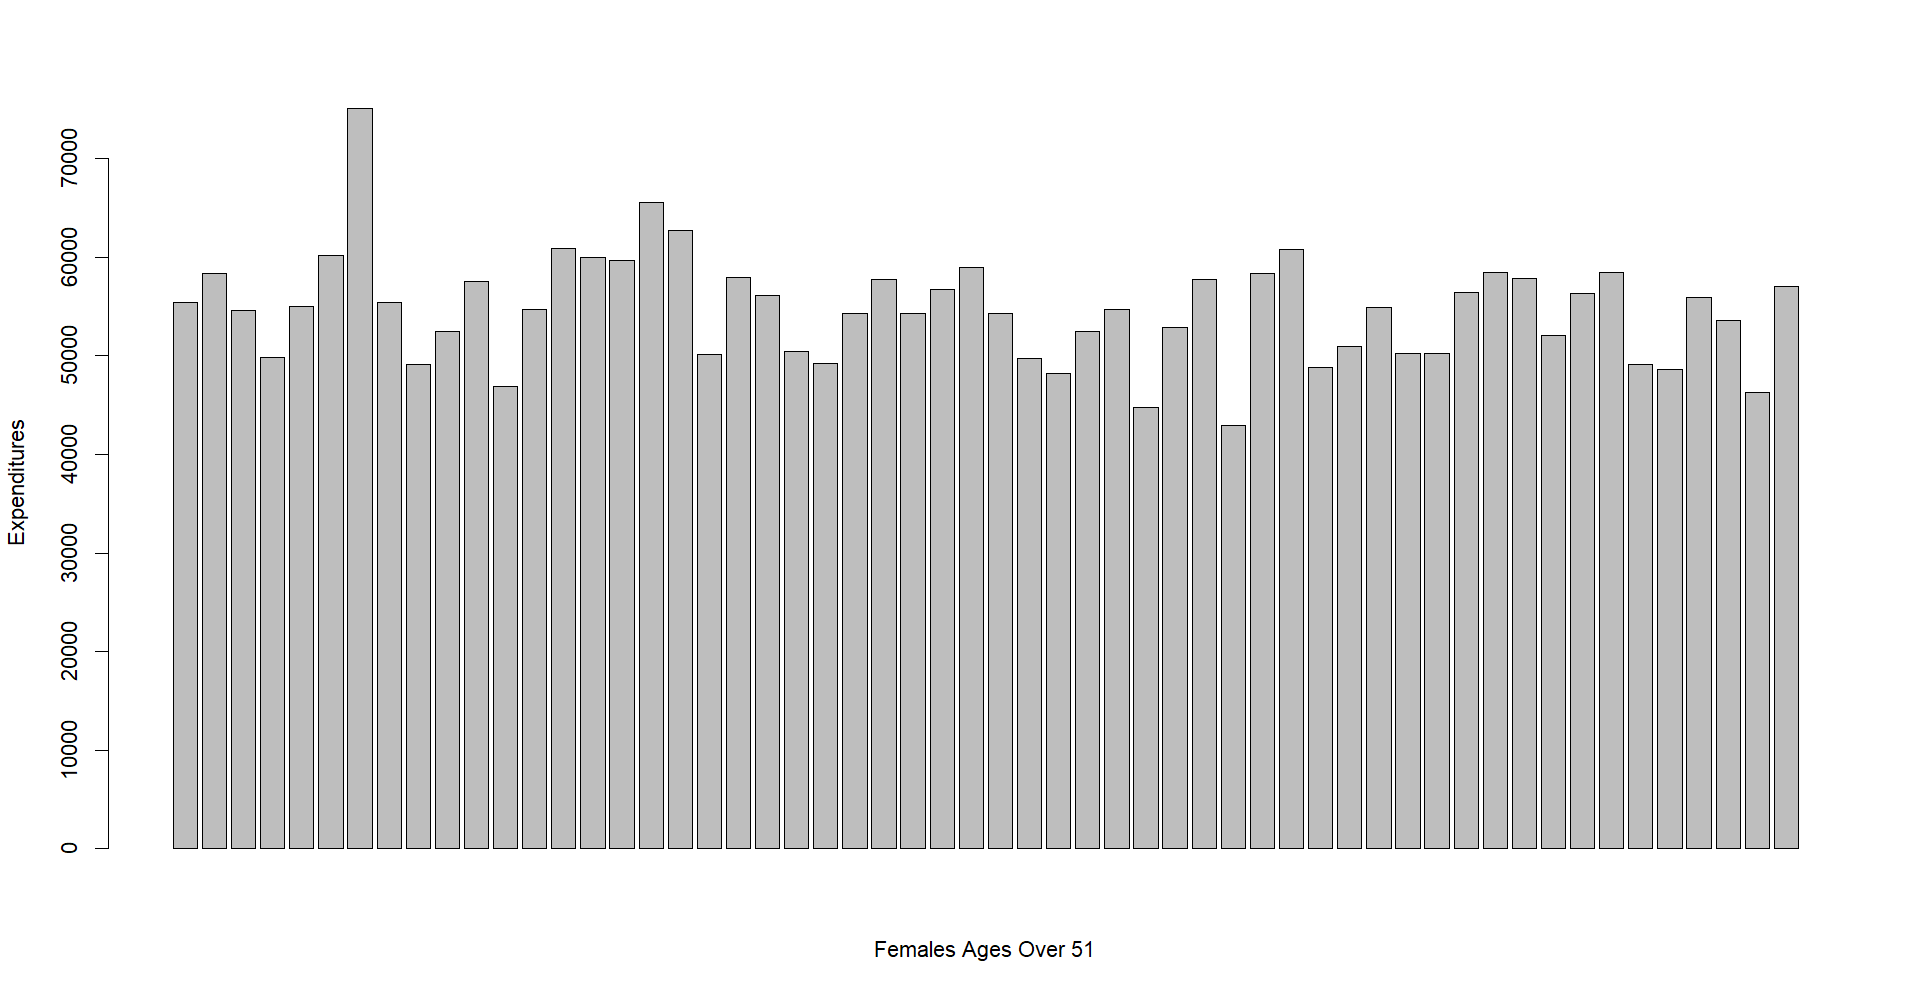
\includegraphics[scale=0.45]{FIG21-Expenditures-Barplot-Female_Over51}
		Figure 21: Expenditures for Females Age Over 51
		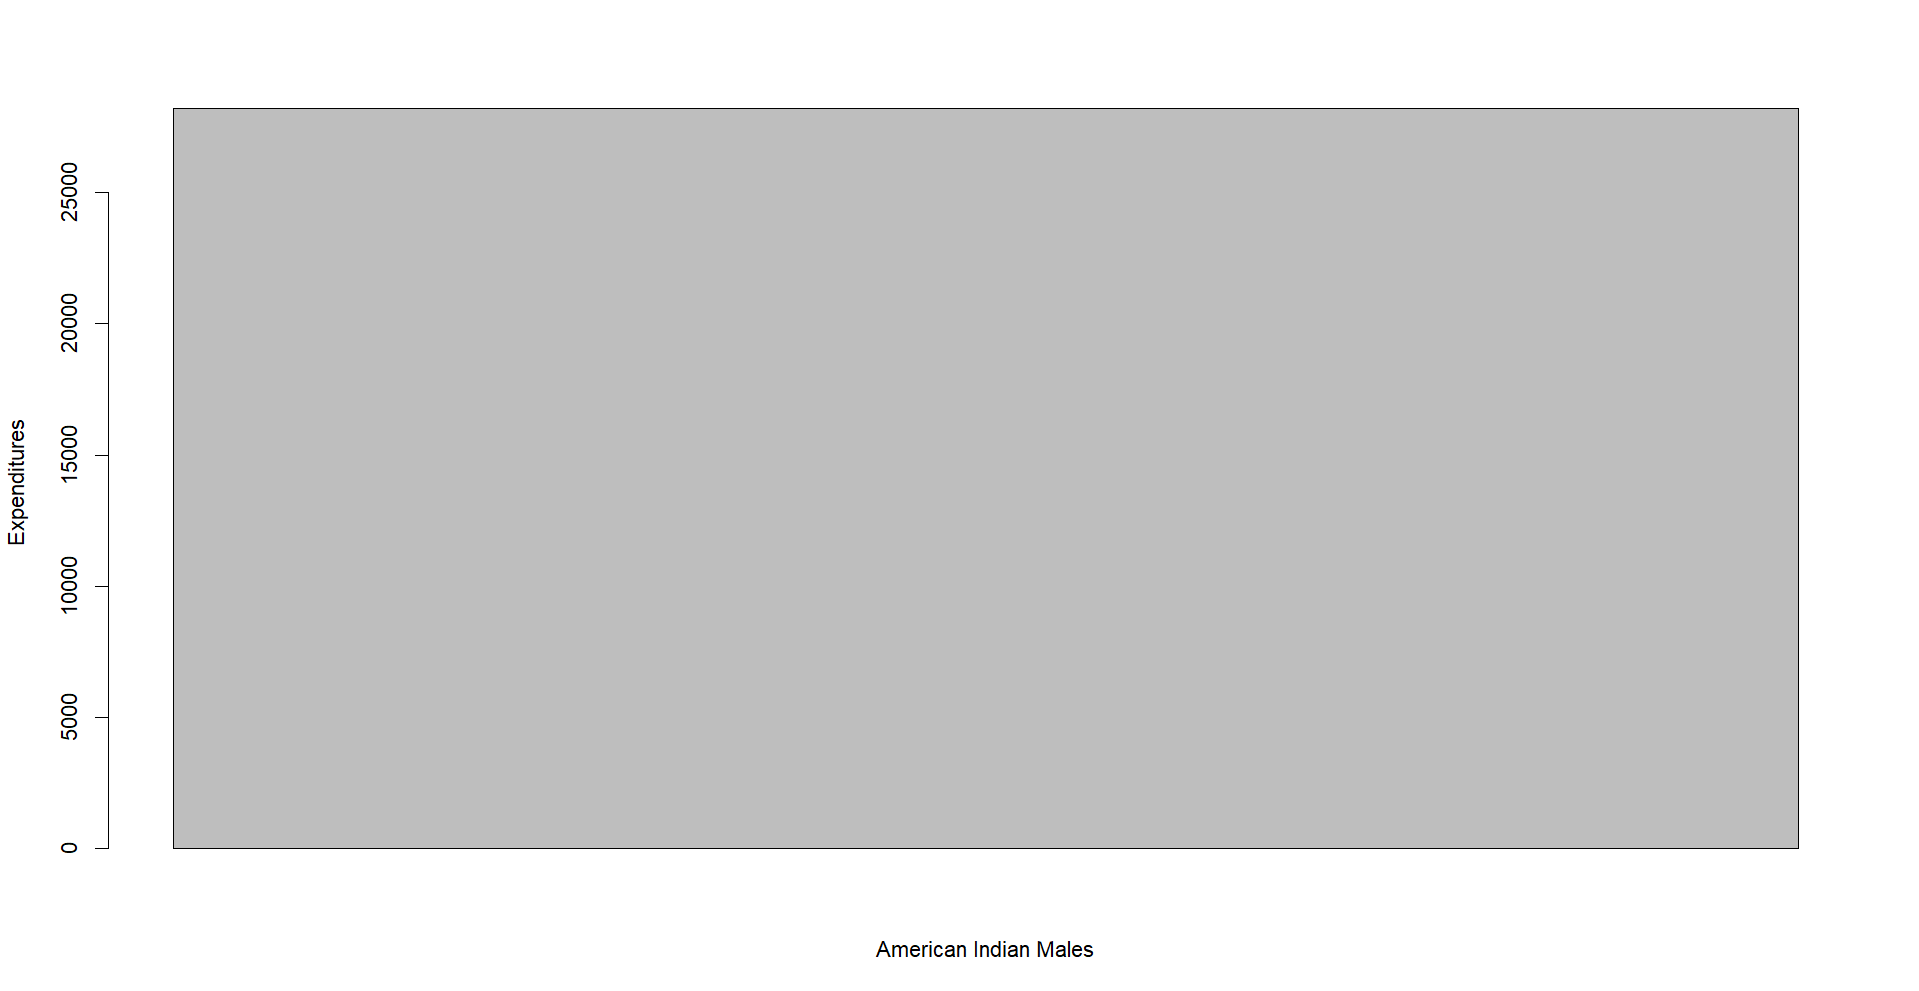
\includegraphics[scale=0.45]{FIG22-Expenditures-Barplot-AmericanIndian_Males}
		Figure 22: Expenditures for American Indian Males
		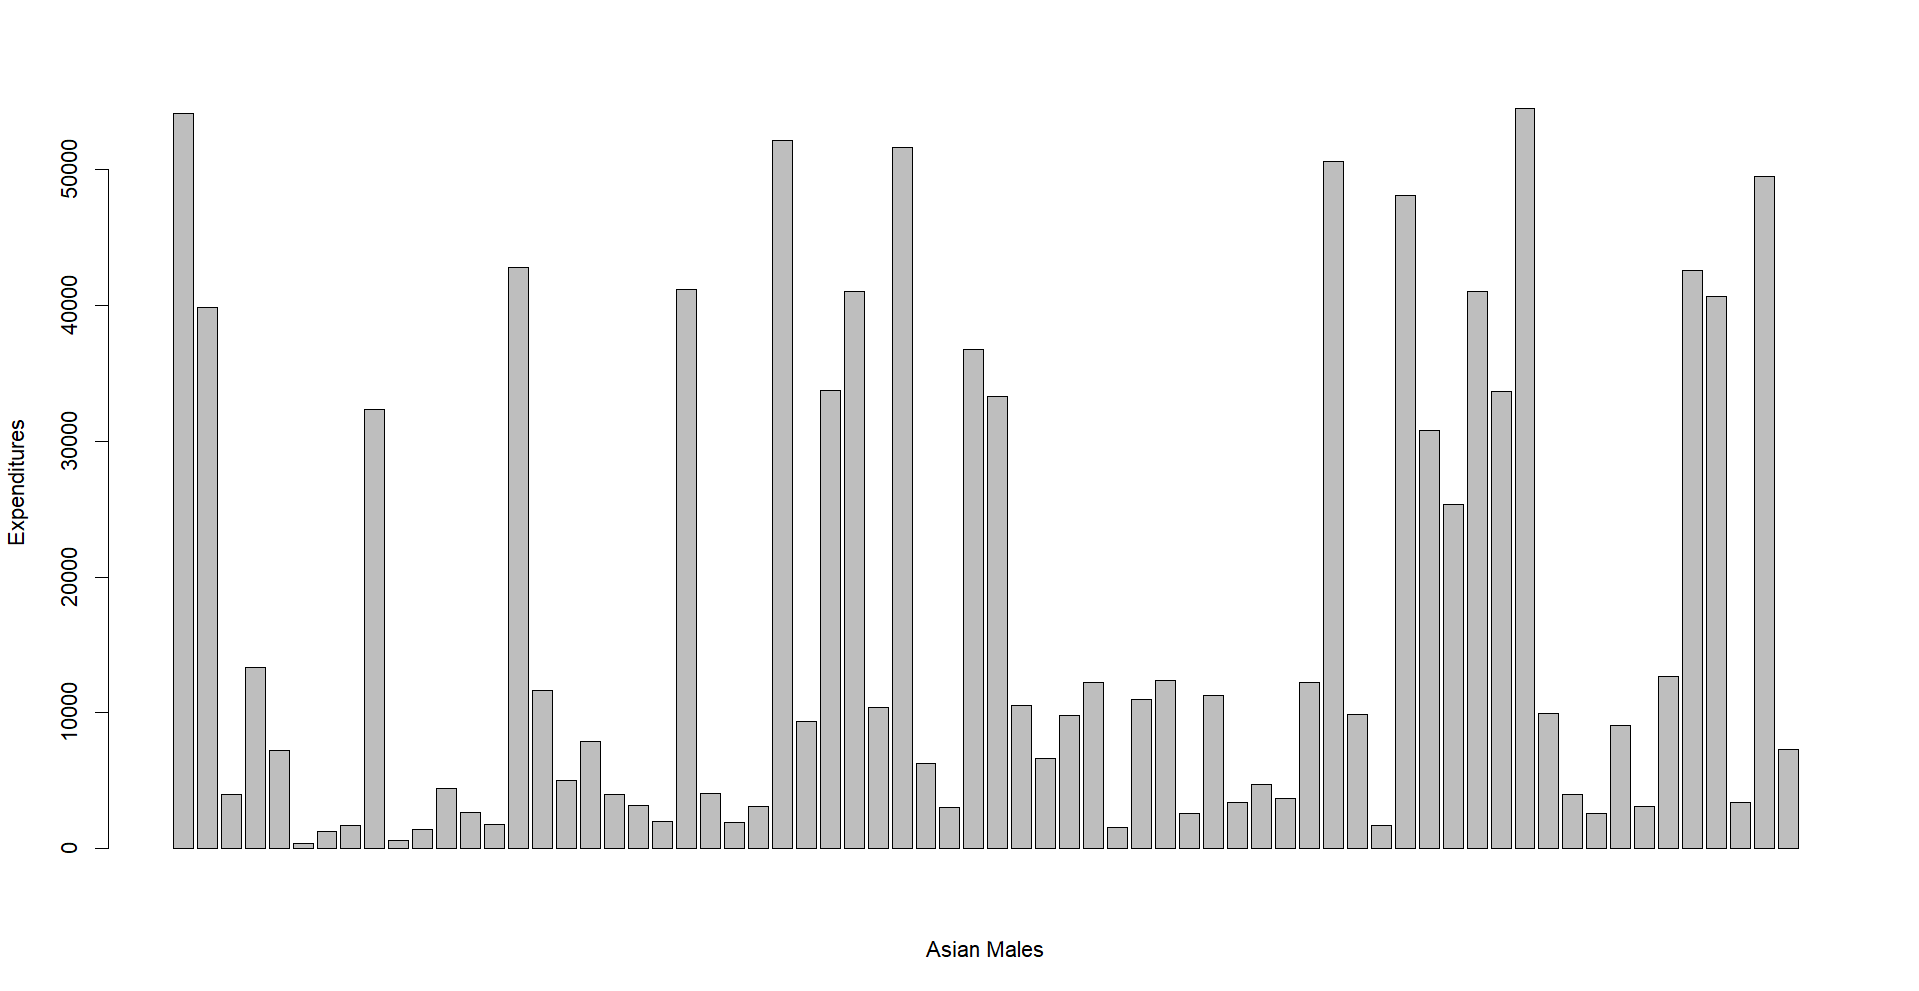
\includegraphics[scale=0.45]{FIG23-Expenditures-Barplot-Asian_Males}
		Figure 23: Expenditures for Asian Males
		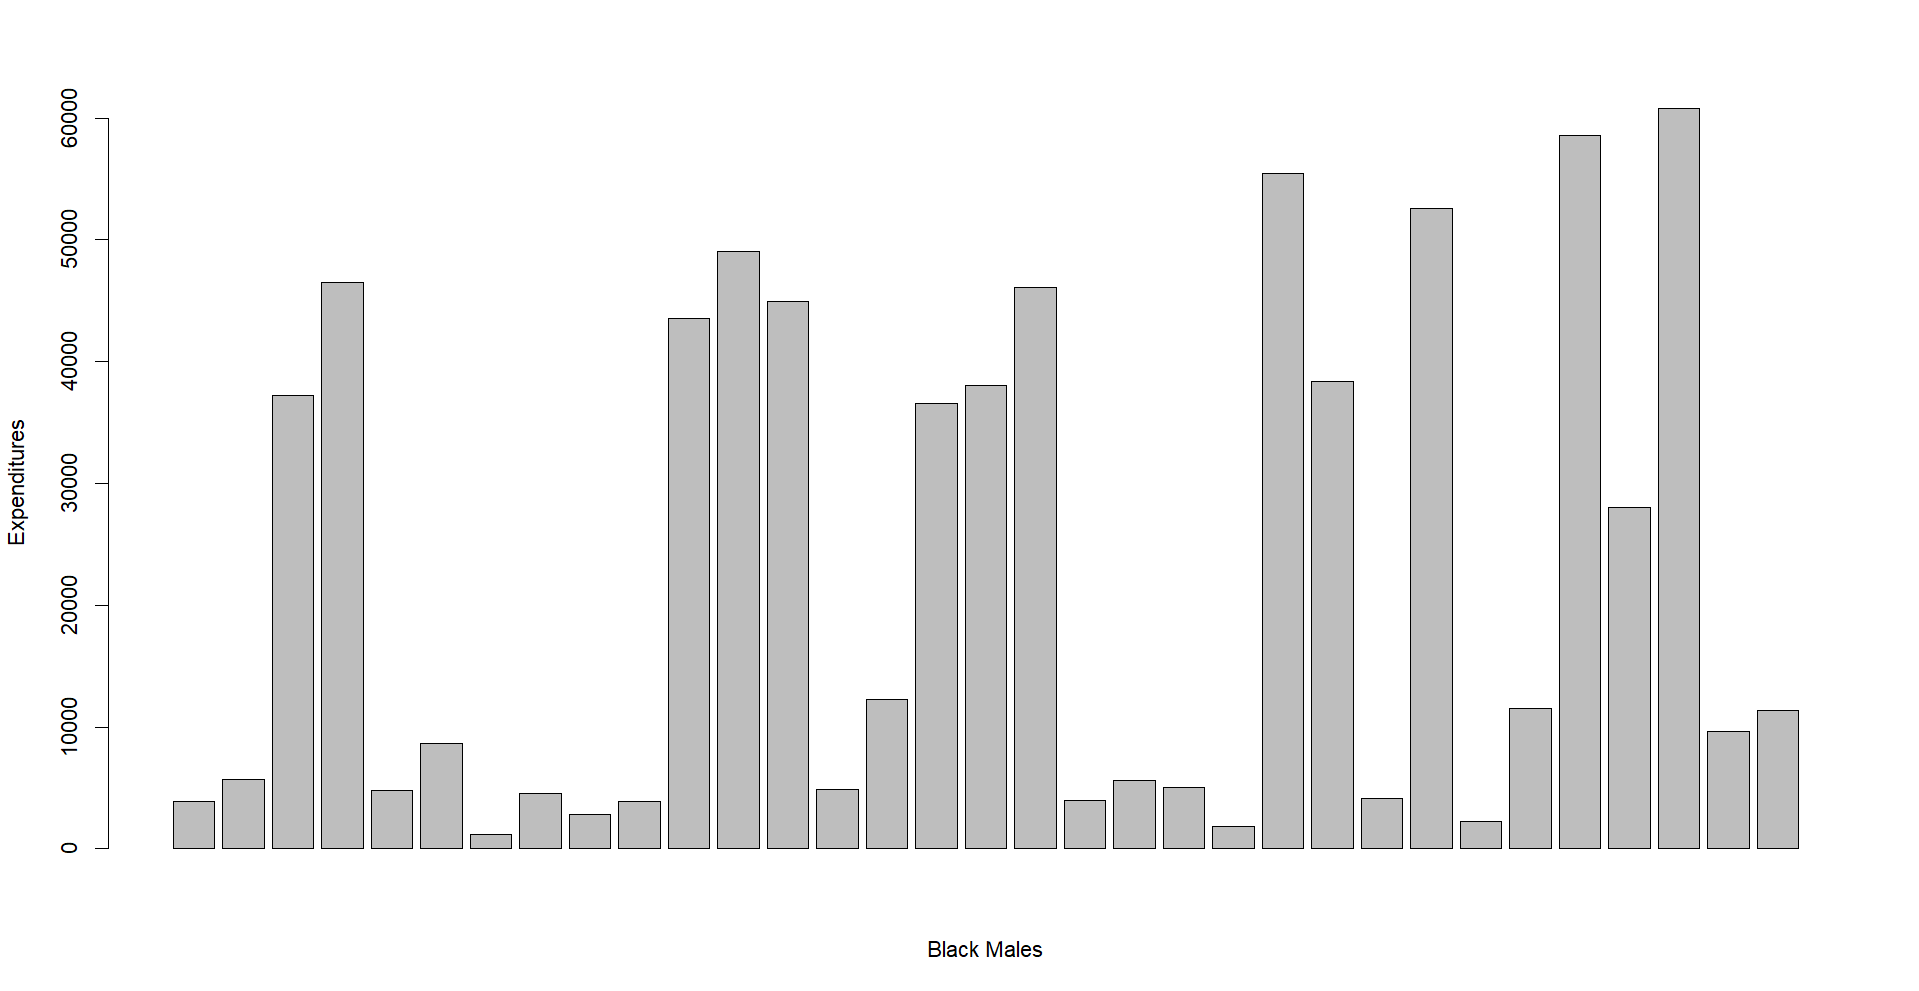
\includegraphics[scale=0.45]{FIG24-Expenditures-Barplot-Black_Males}
		Figure 24: Expenditures for Black Males
		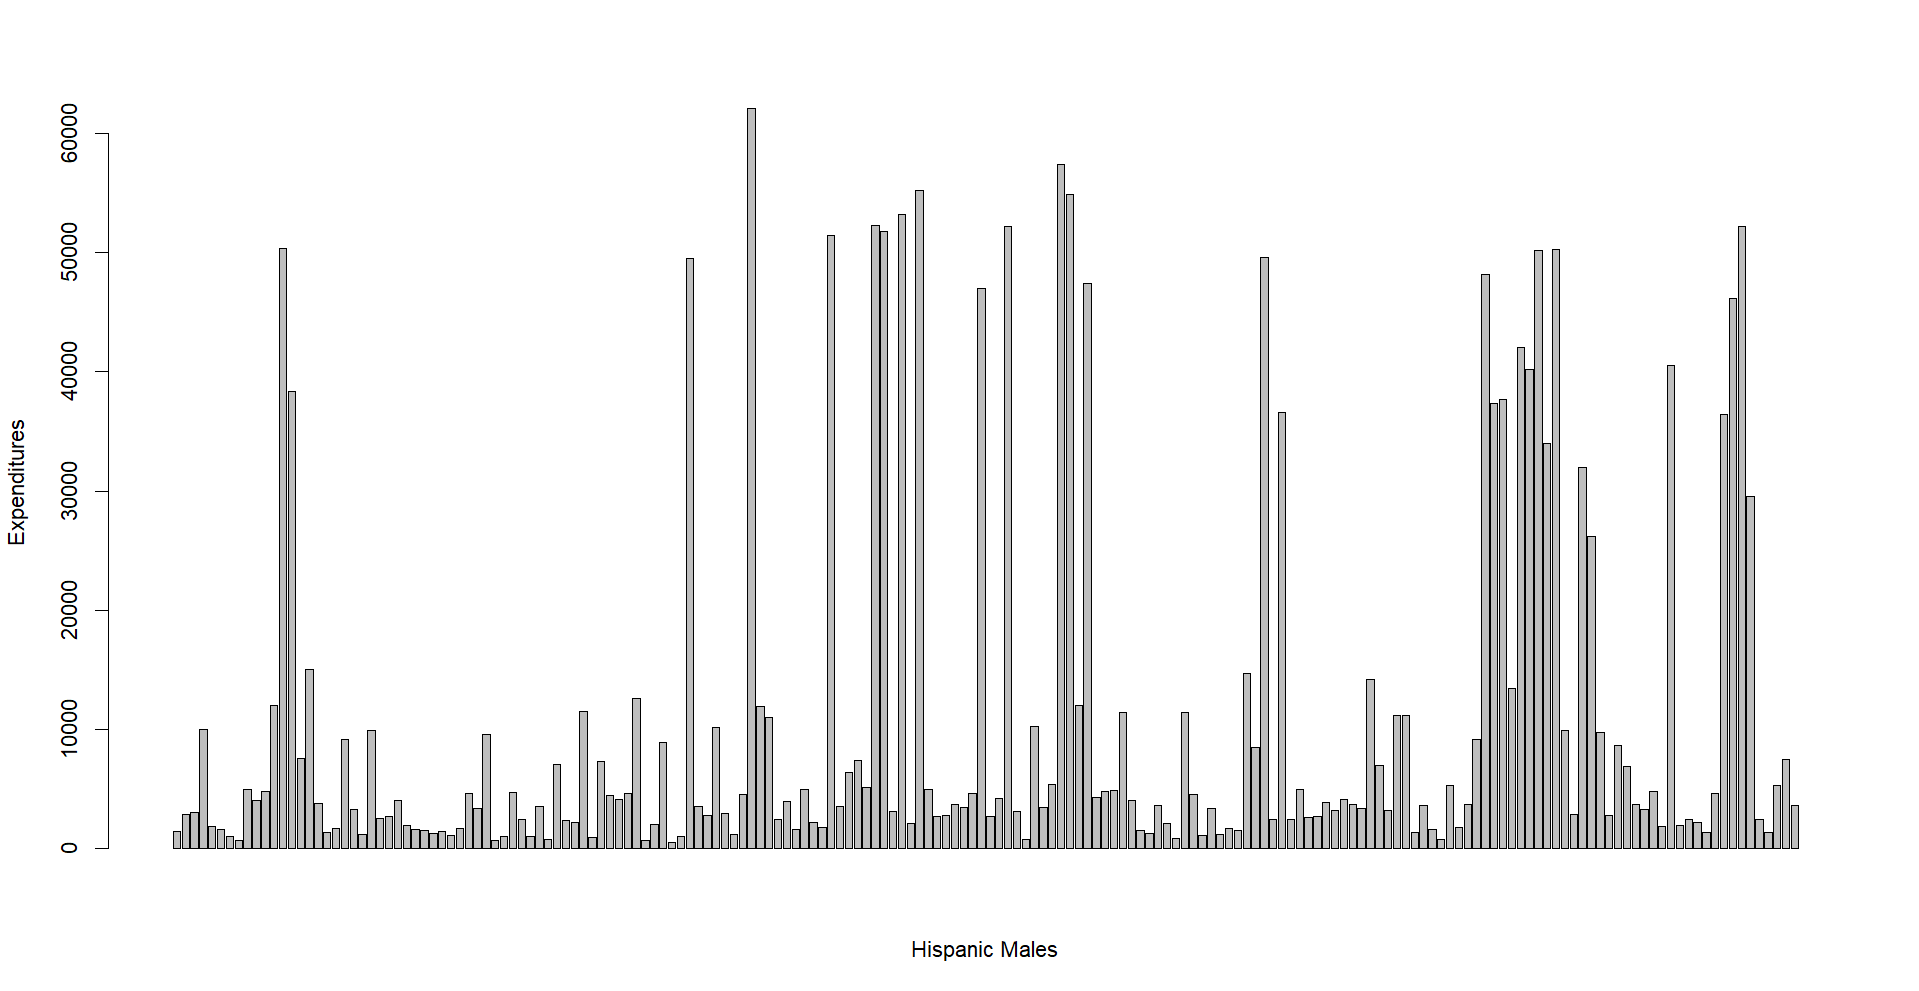
\includegraphics[scale=0.45]{FIG25-Expenditures-Barplot-Hispanic_Males}
		Figure 25: Expenditures for Hispanic Males
		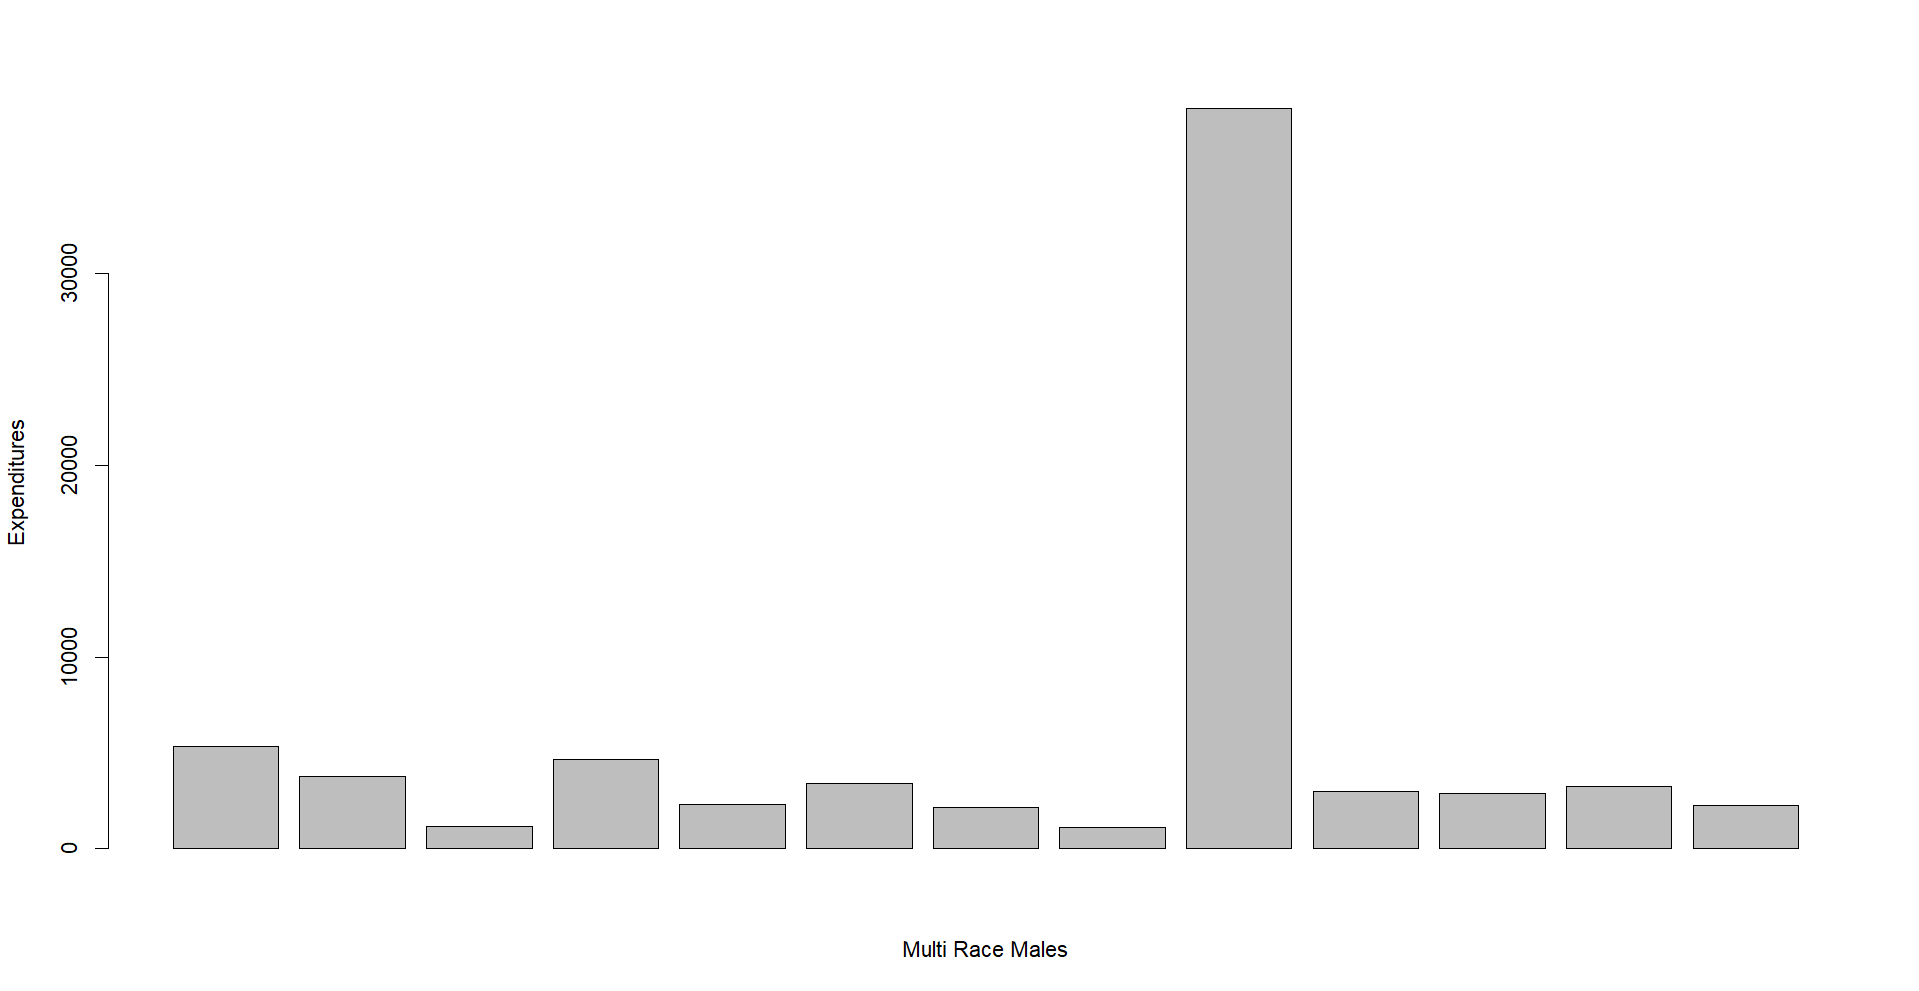
\includegraphics[scale=0.45]{FIG26-Expenditures-Barplot-MultiRace_Males}
		Figure 26: Expenditures for Multi Race Males
		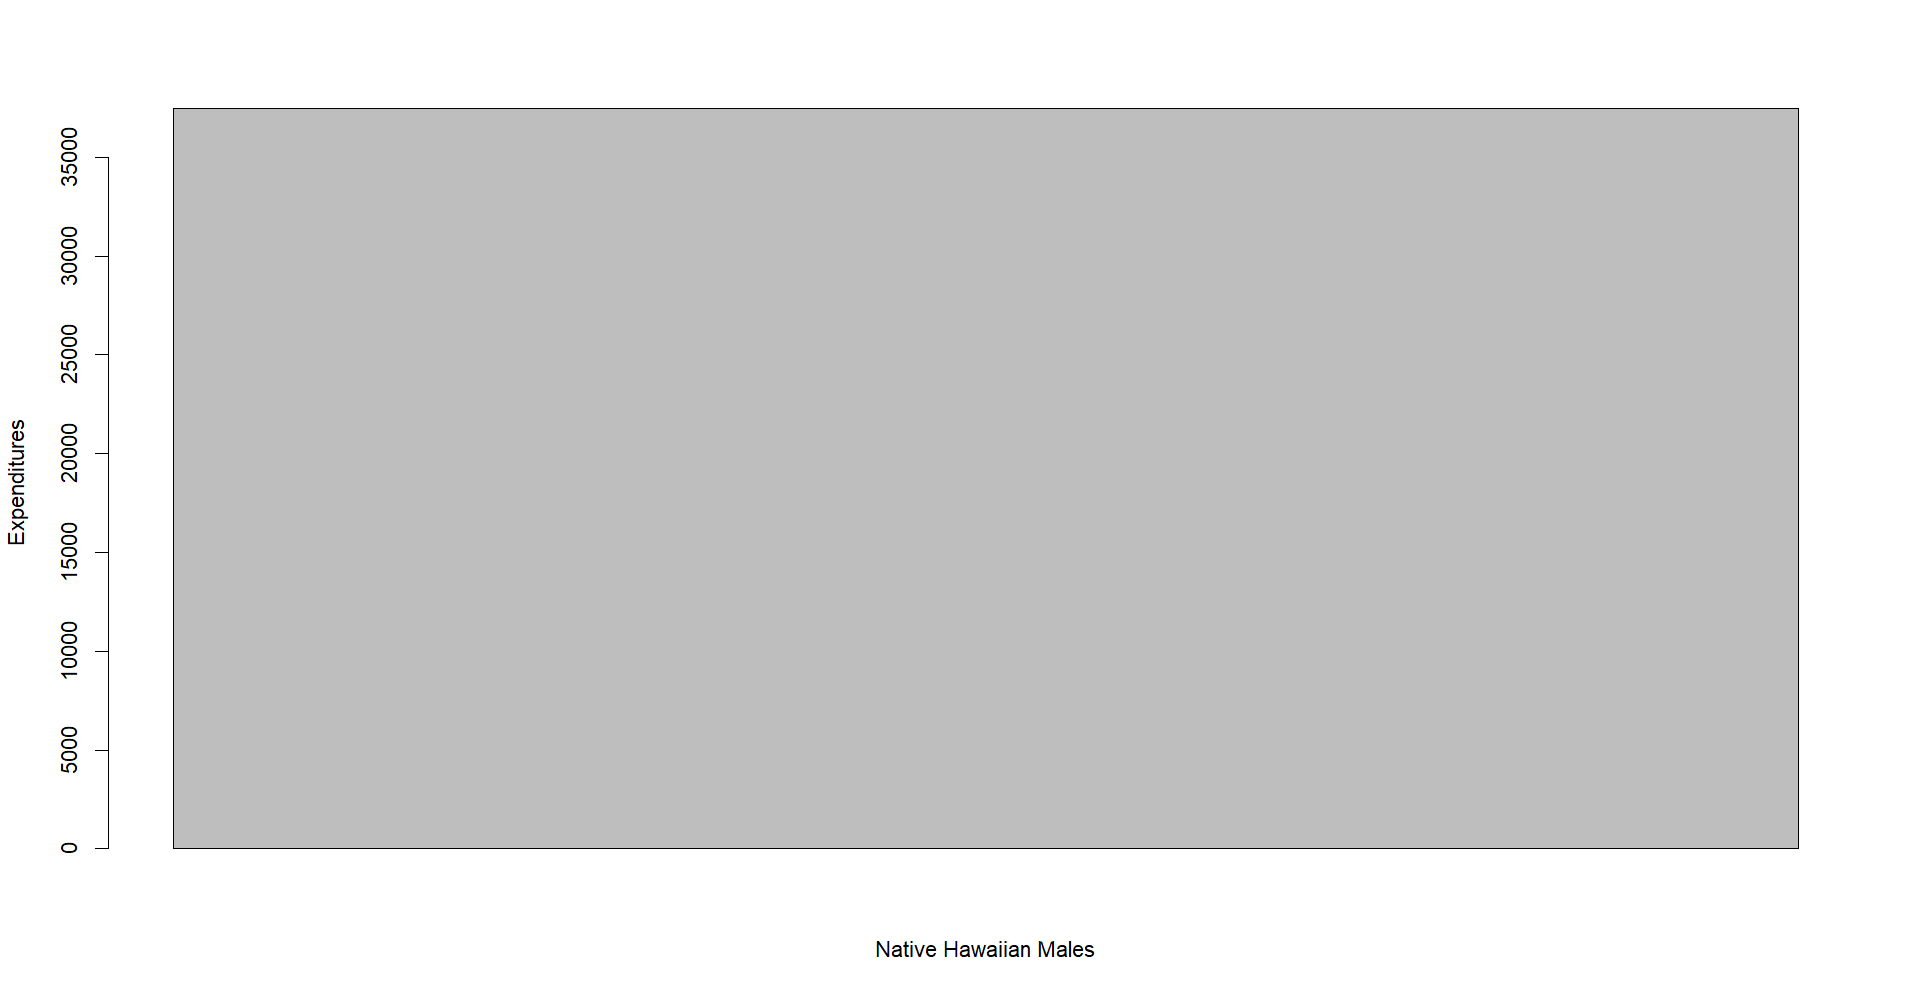
\includegraphics[scale=0.45]{FIG27-Expenditures-Barplot-NativeHawaiian_Males}
		Figure 27: Expenditures for Native Hawaiian Males
		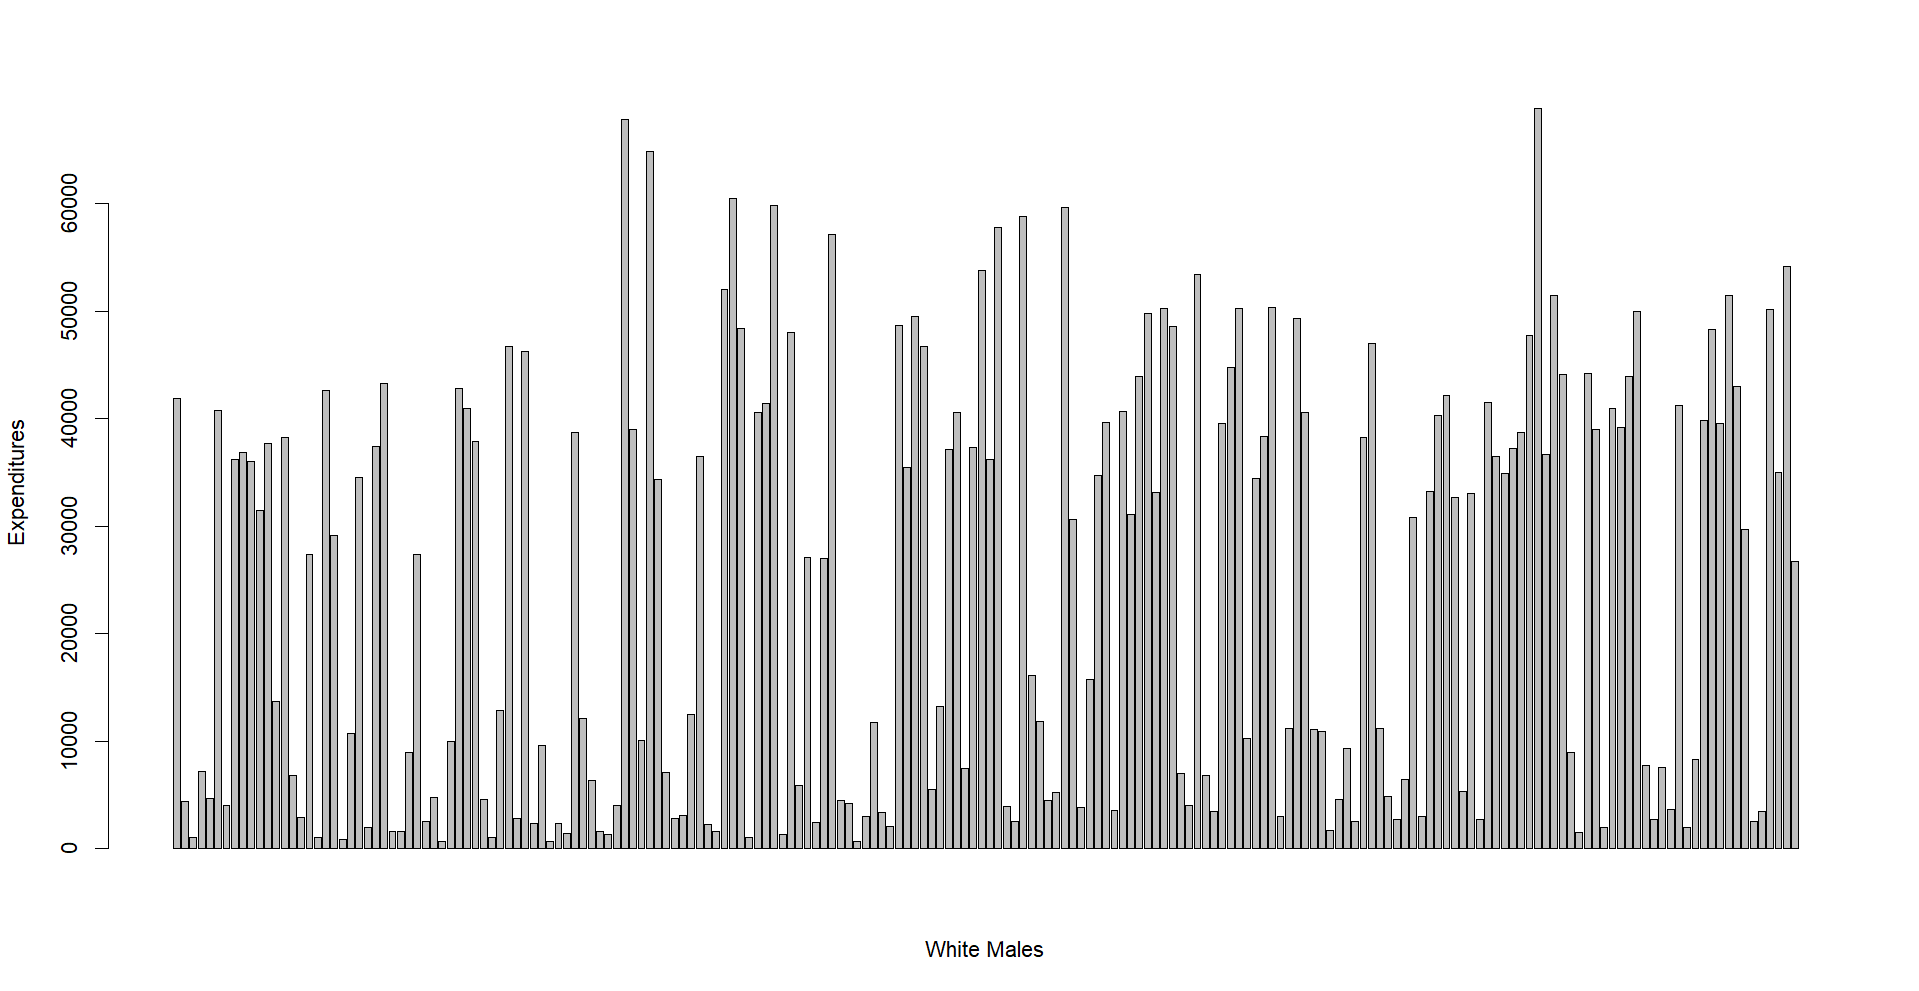
\includegraphics[scale=0.45]{FIG28-Expenditures-Barplot-White_Males}
		Figure 28: Expenditures for White not Hispanic Males
		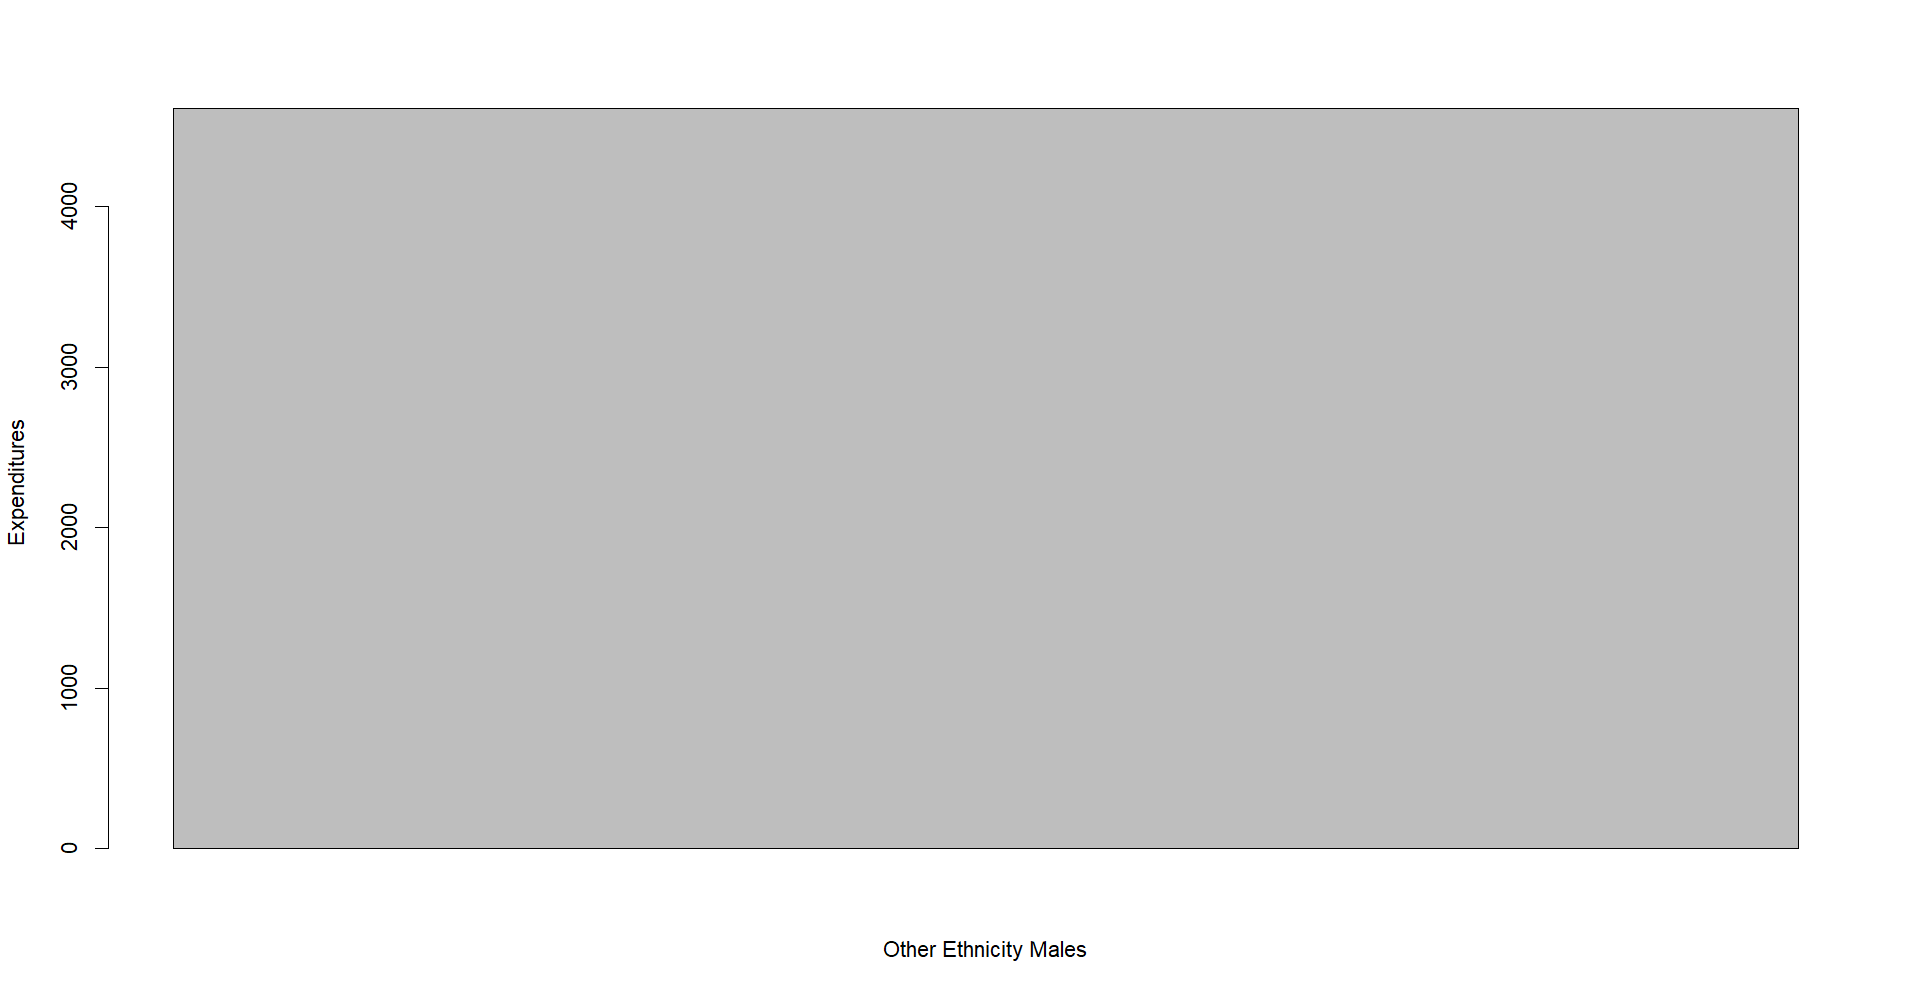
\includegraphics[scale=0.45]{FIG29-Expenditures-Barplot-OtherEthnicity_Males}
		Figure 29: Expenditures for Males of Other Ethnicities
		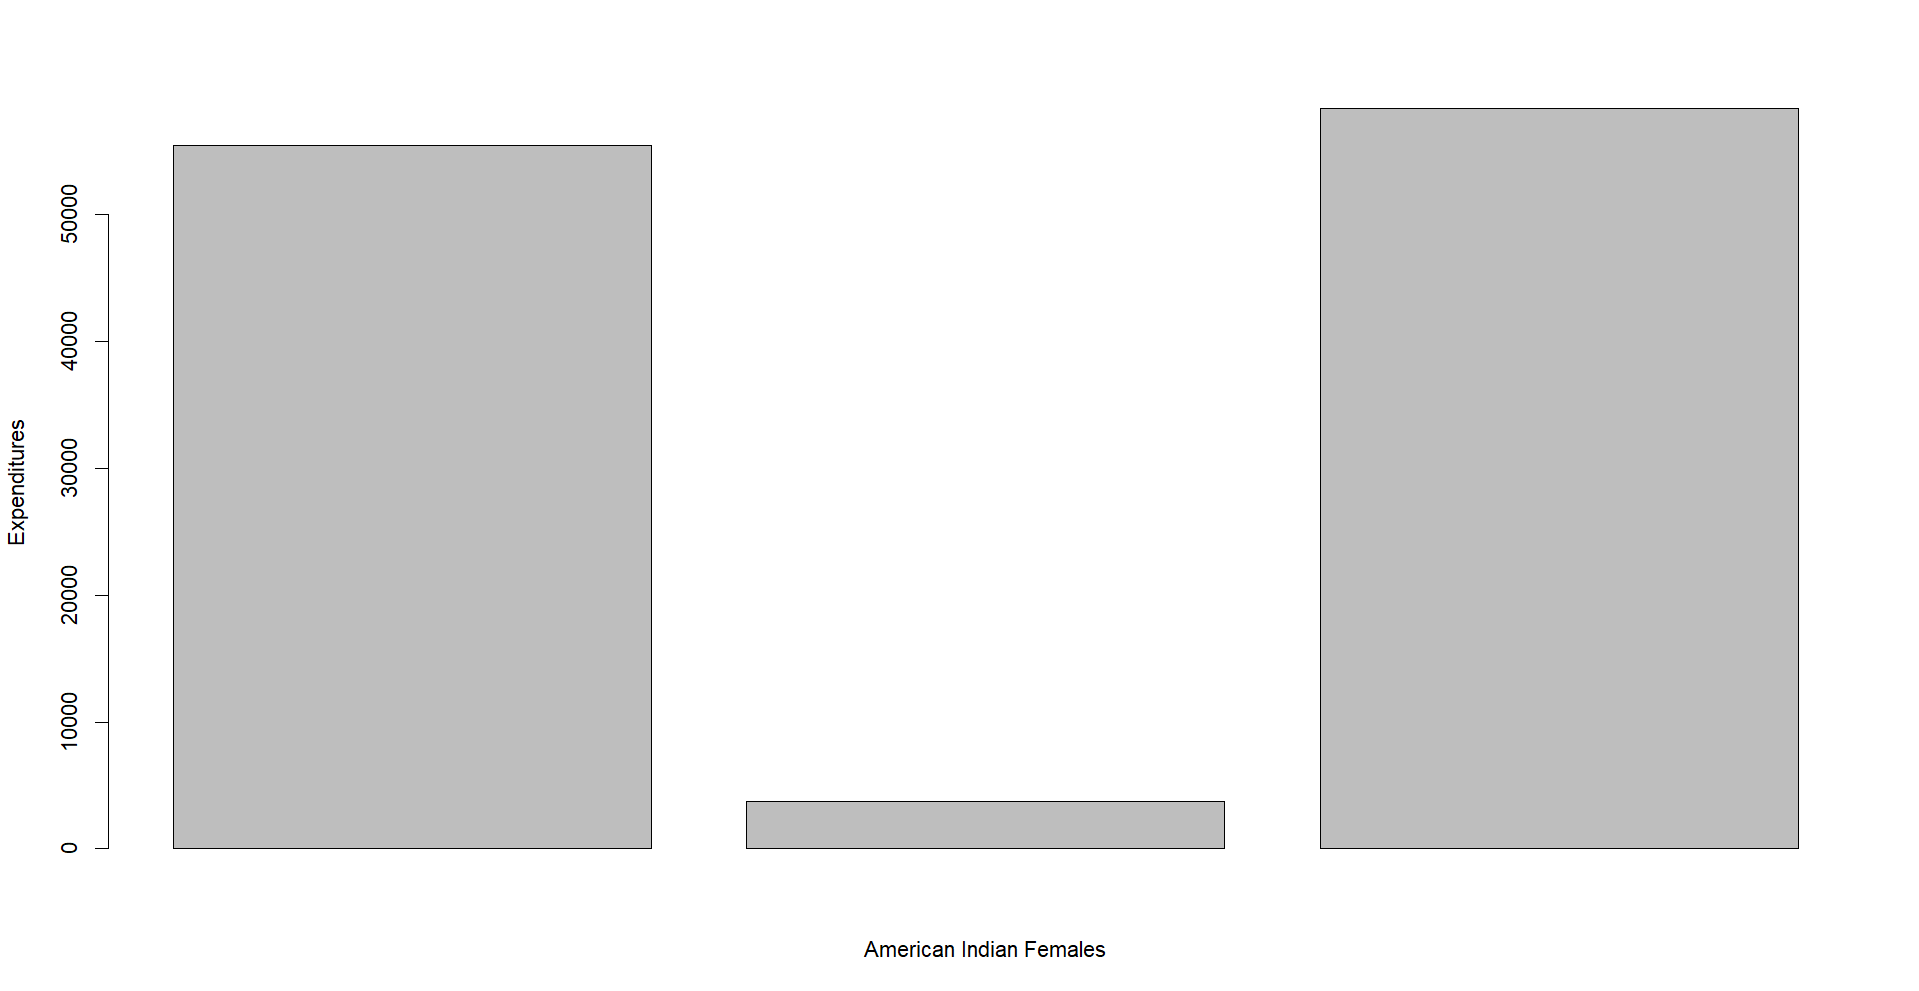
\includegraphics[scale=0.45]{FIG30-Expenditures-Barplot-AmericanIndian_Females}
		Figure 30: Expenditures for American Indian Females
		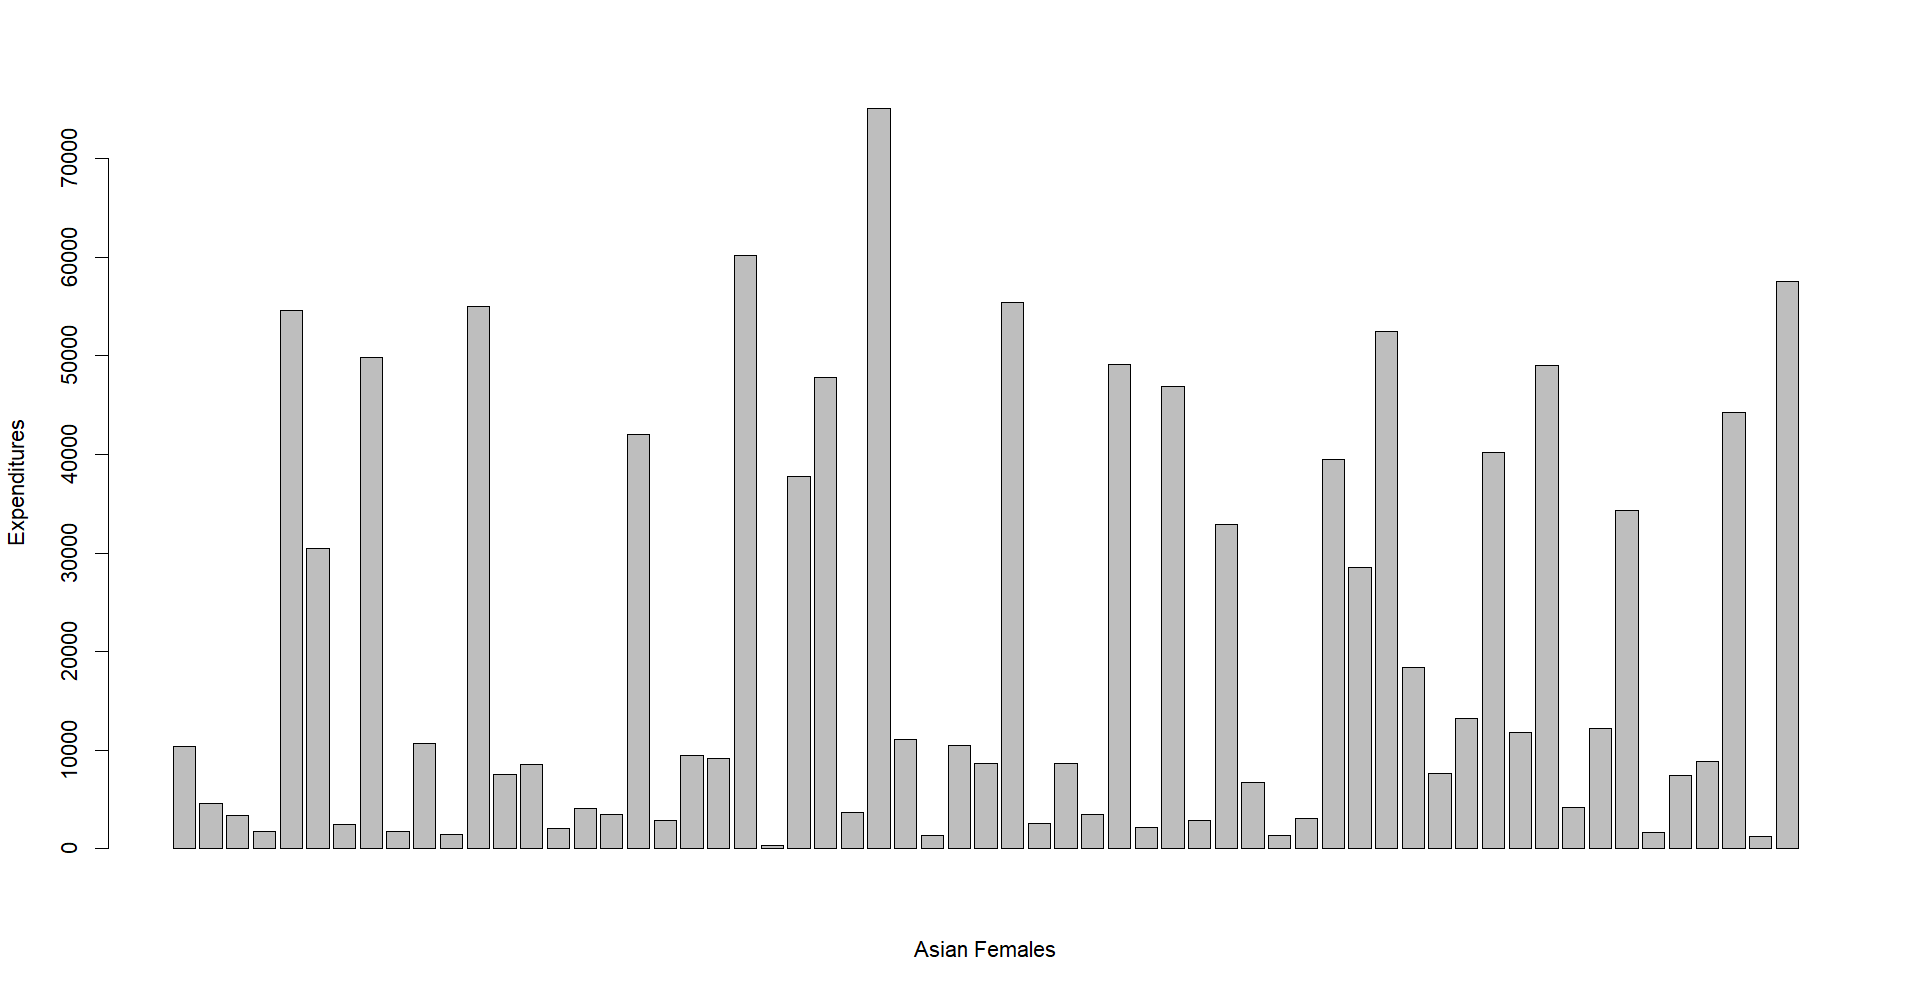
\includegraphics[scale=0.45]{FIG31-Expenditures-Barplot-Asian_Females}
		Figure 31: Expenditures for Asian Females
		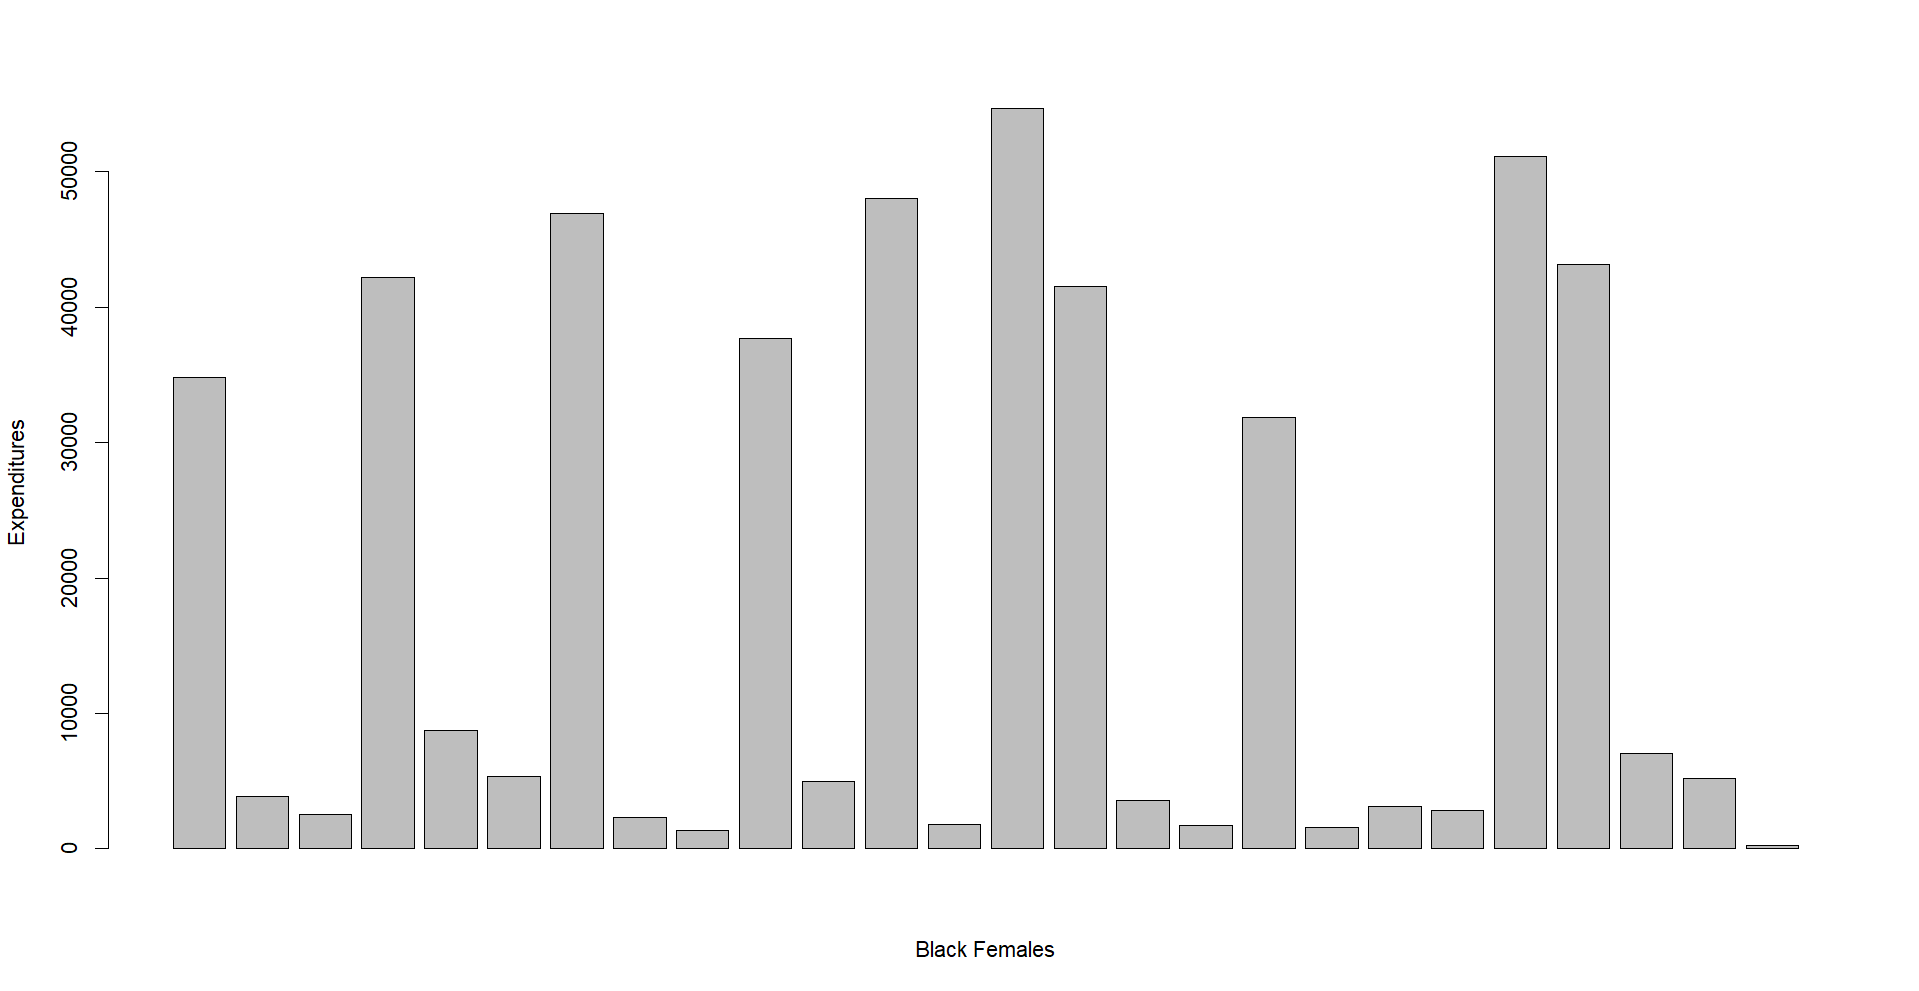
\includegraphics[scale=0.45]{FIG32-Expenditures-Barplot-Black_Females}
		Figure 32: Expenditures for Black Females
		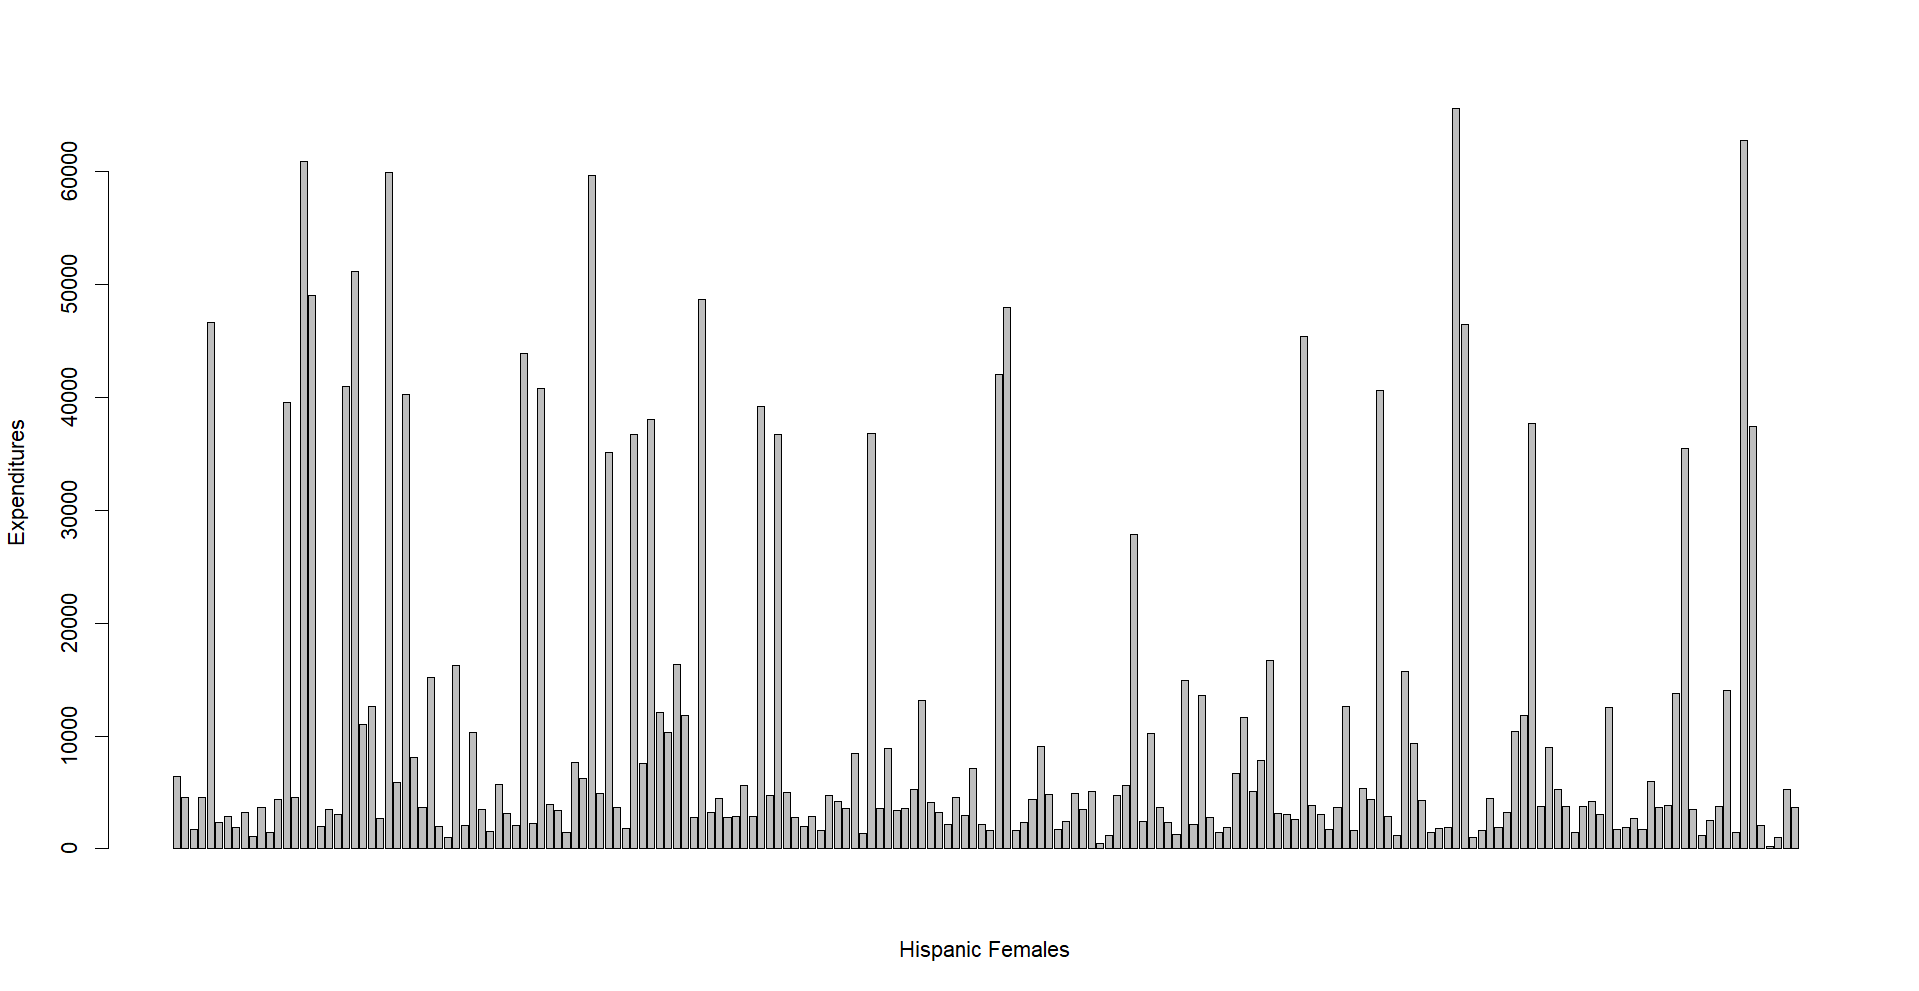
\includegraphics[scale=0.45]{FIG33-Expenditures-Barplot-Hispanic_Females}
		Figure 33: Expenditures for Hispanic Females
		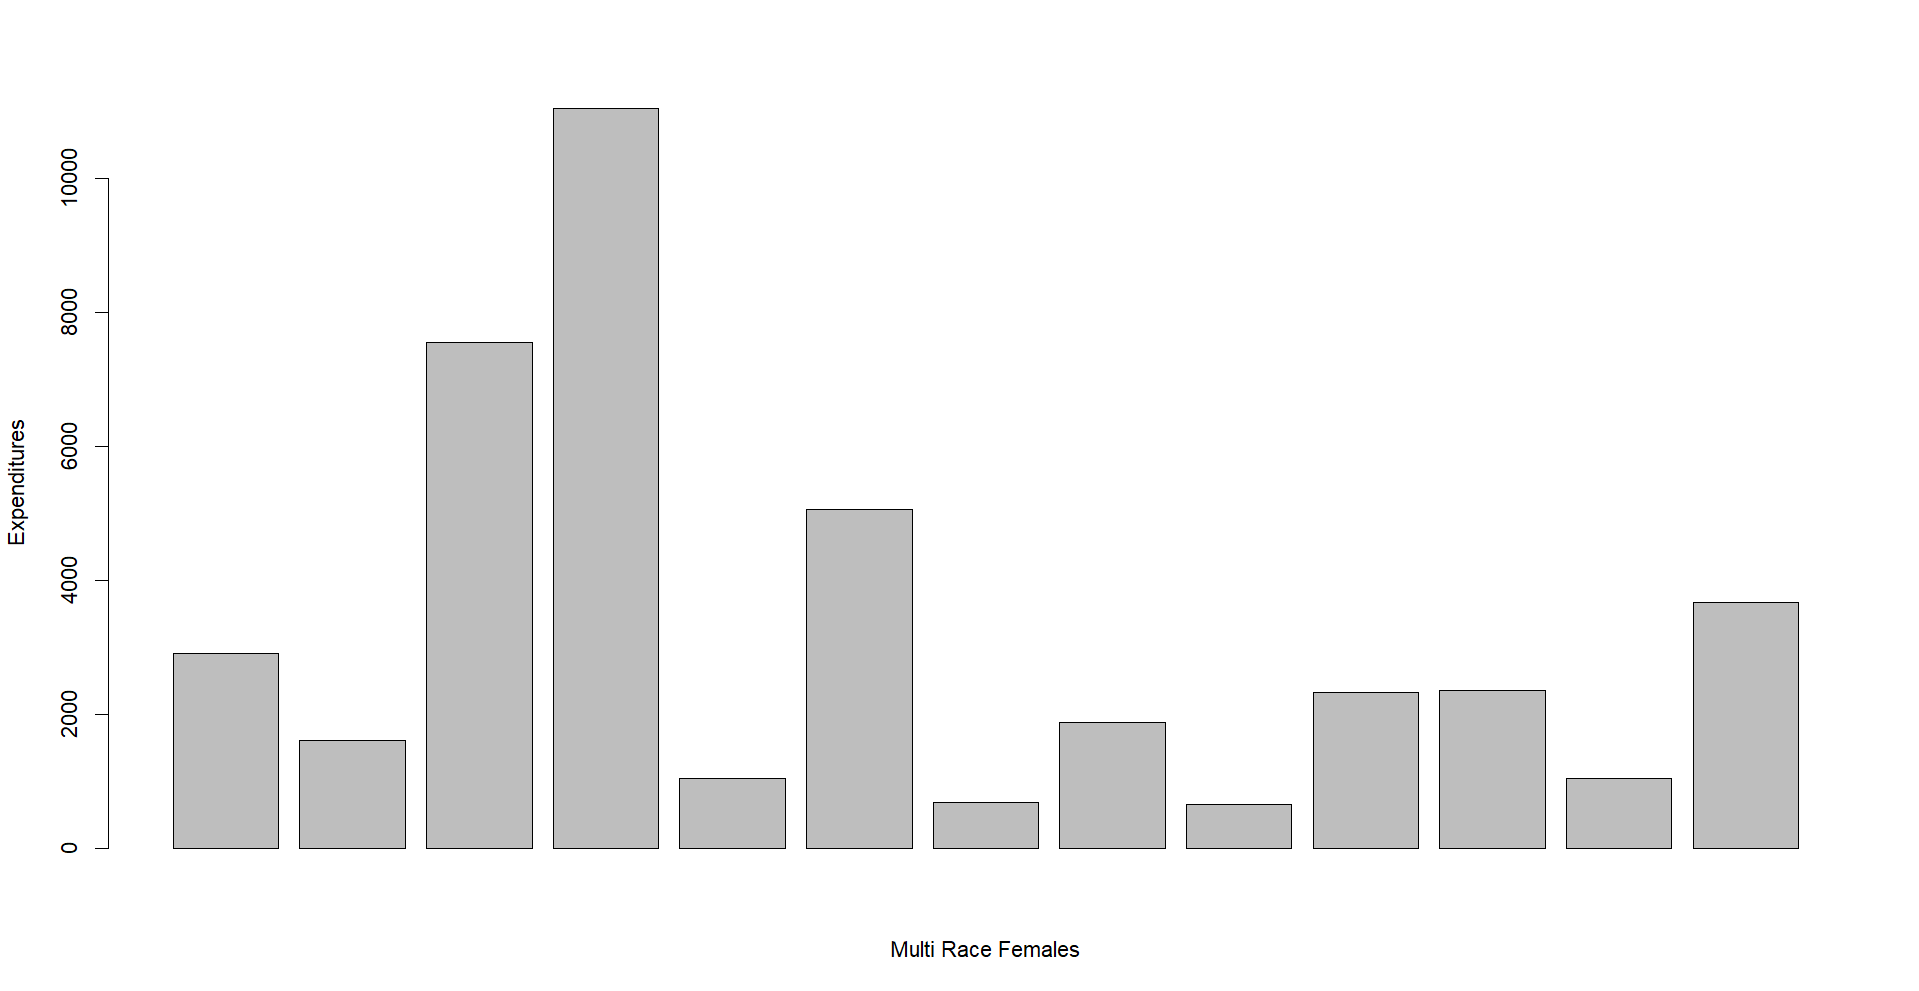
\includegraphics[scale=0.45]{FIG34-Expenditures-Barplot-MultiRace_Females}
		Figure 34: Expenditures for Multi Race Females
		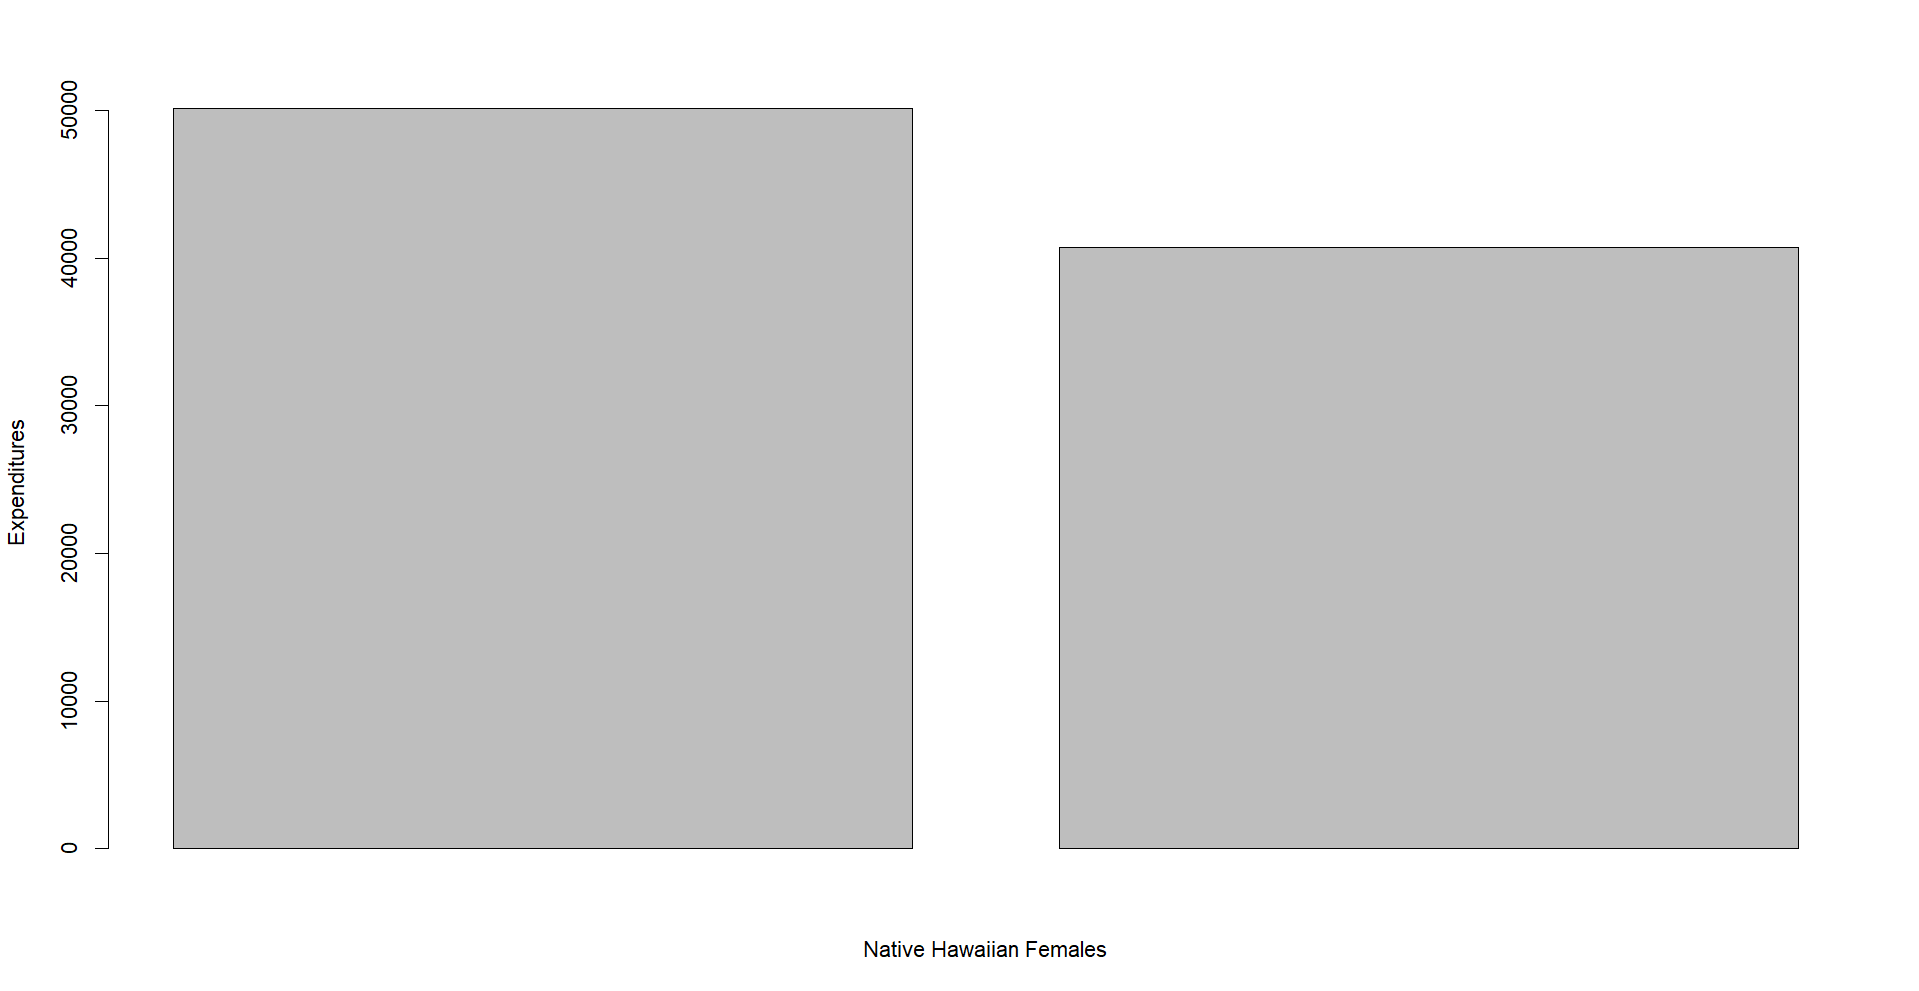
\includegraphics[scale=0.45]{FIG35-Expenditures-Barplot-NativeHawaiian_Females}
		Figure 35: Expenditures for Native Hawaiian Females
		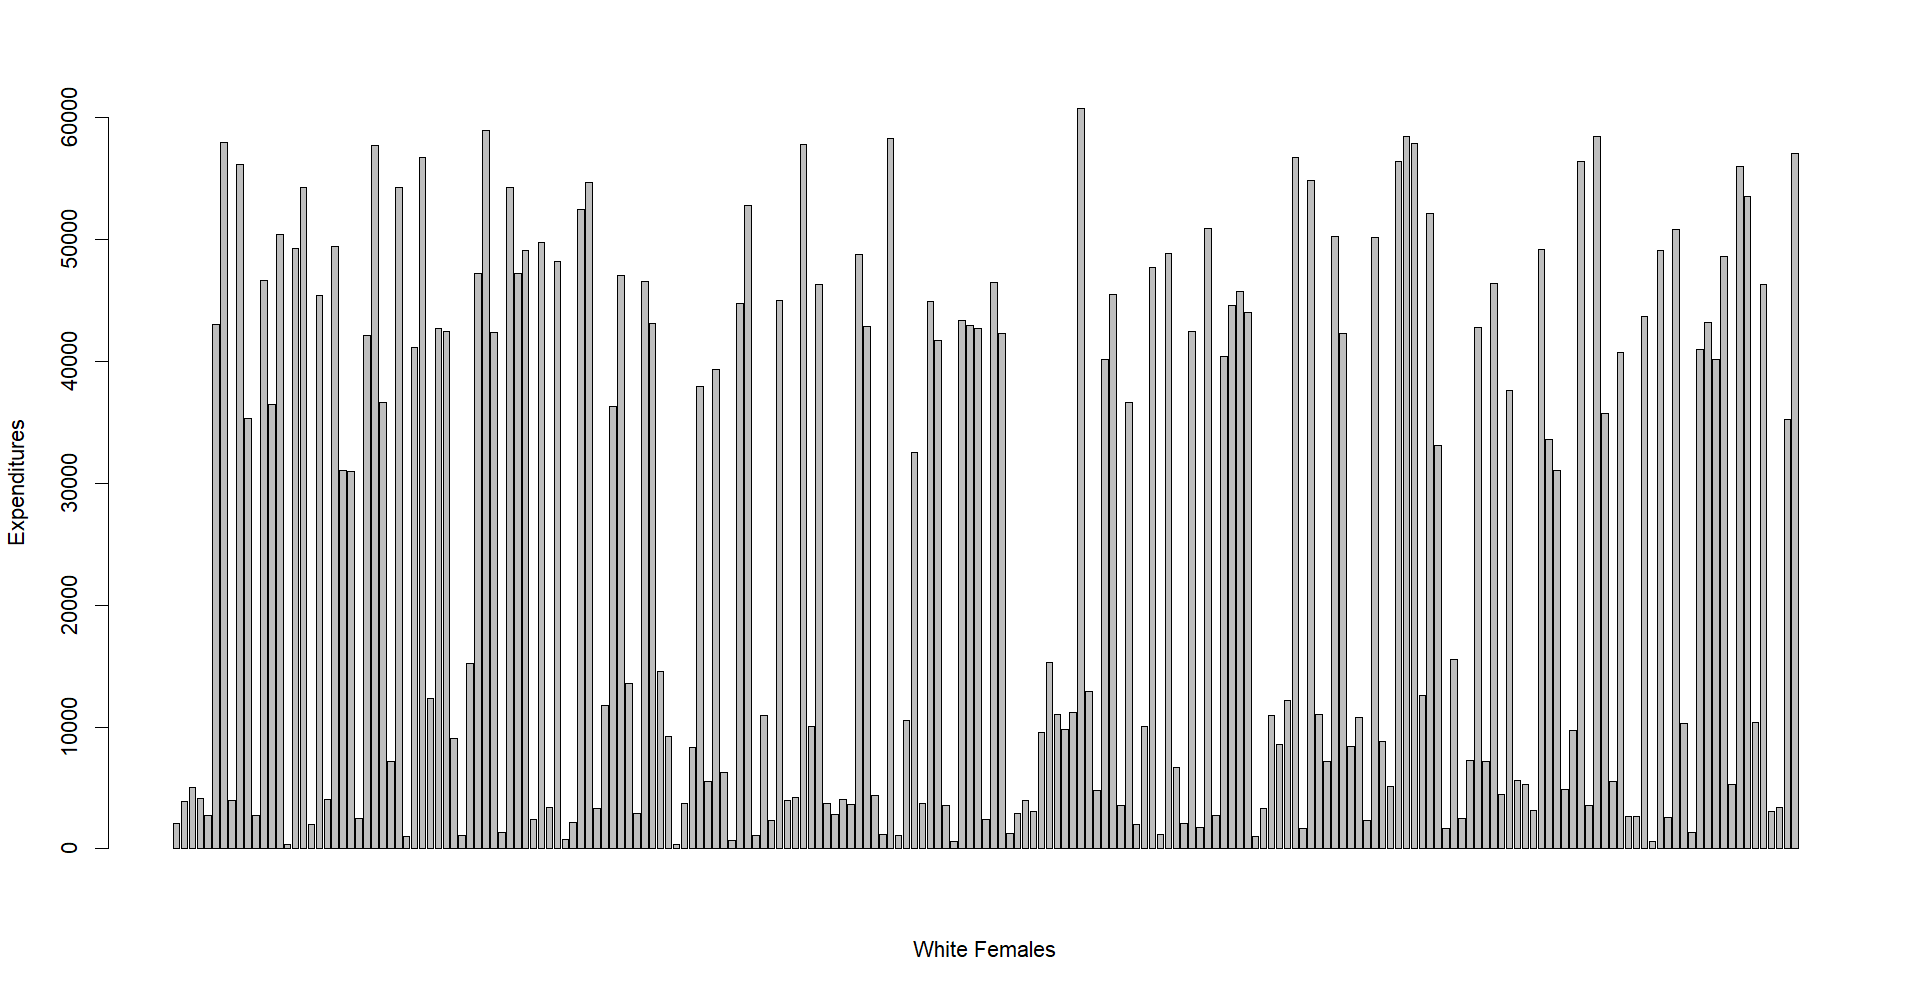
\includegraphics[scale=0.45]{FIG36-Expenditures-Barplot-White_Females}
		Figure 36: Expenditures for White not Hispanic Females
		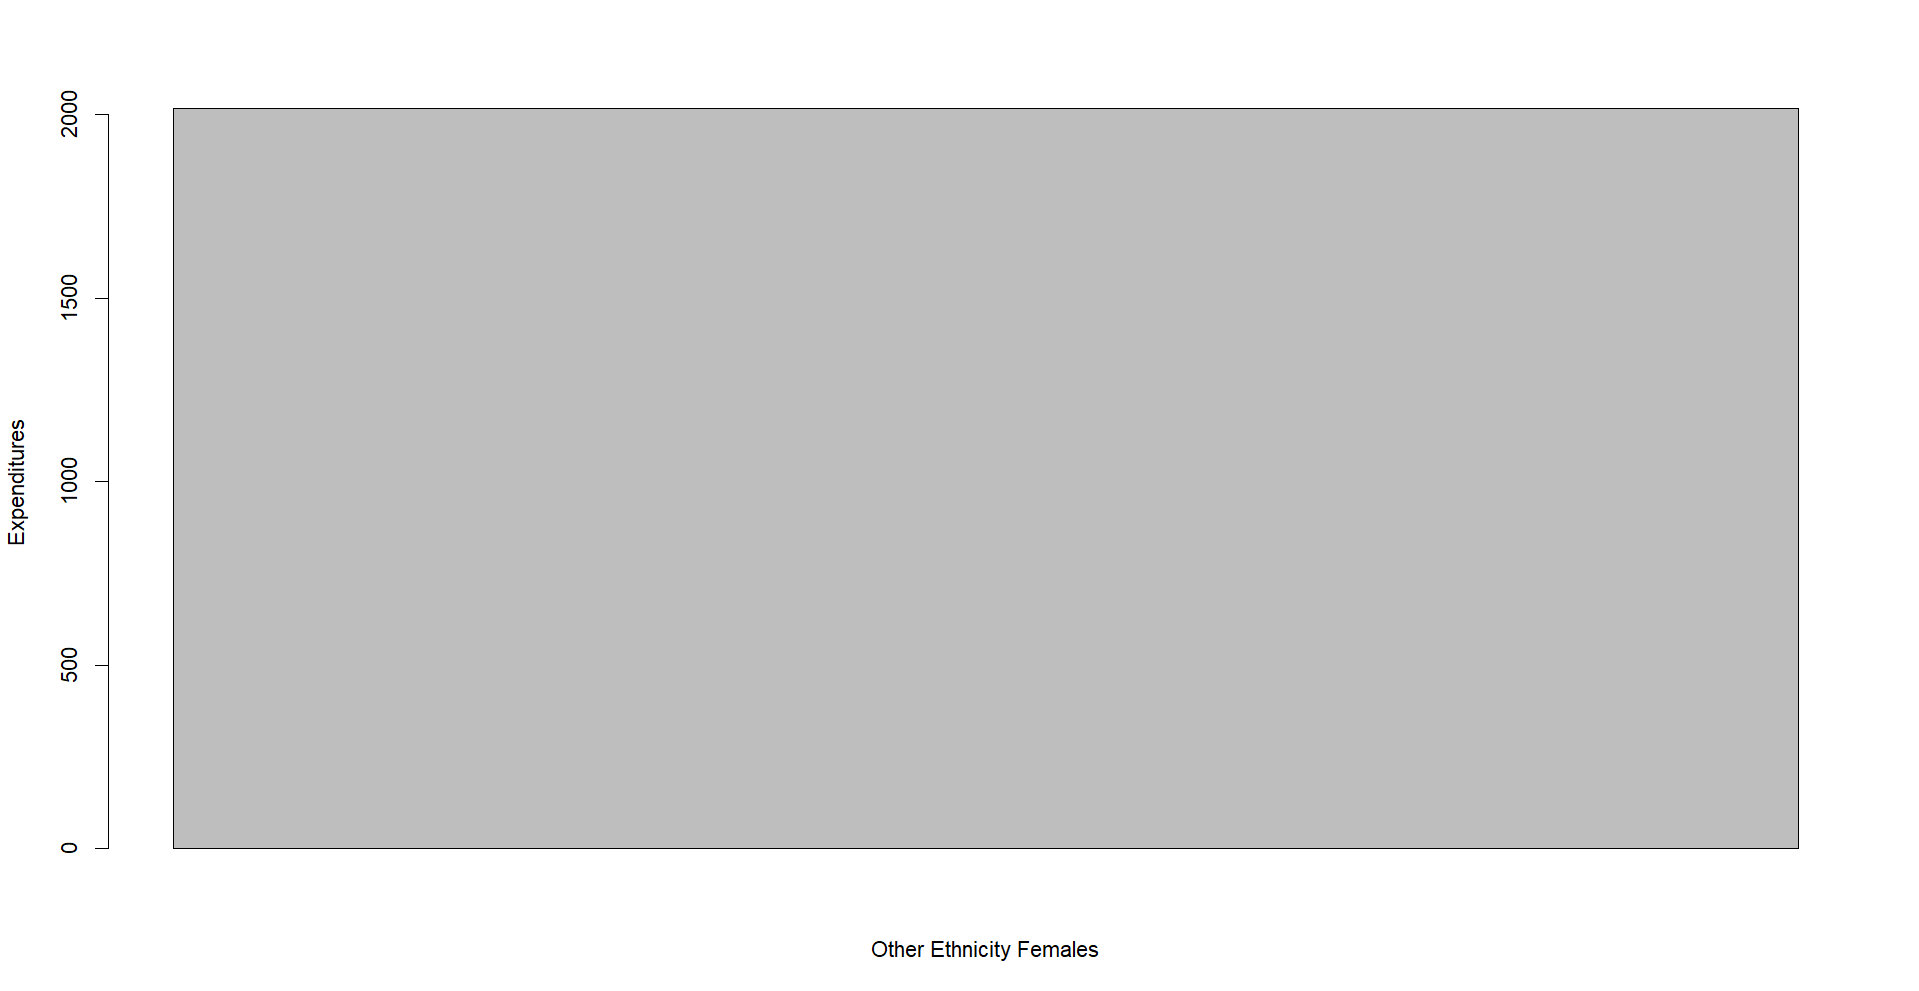
\includegraphics[scale=0.45]{FIG37-Expenditures-Barplot-OtherEthnicity_Females}
		Figure 37: Expenditures for Females of Other Ethnicities
	\end{center}
	\subsection{R Code}
	\setlength{\parindent}{3em}
	\singlespacing
	\mycourier{
		\# Read in data\\
		data <- read.csv("California\_DDS\_Expenditures.csv")\\
		View(data)\\
		\ \\
		\# Side-by-side boxplots of expenditures by Ethnicity\\
		boxplot(data\$Expenditures$\sim$data\$Ethnicity, xlab="Ethnicity",\\
		\indent ylab="Expenditures")\\
		\ \\
		\# Subset data to only White not Hispanic and Hispanic\\
		data.White <- subset(data, Ethnicity == "White not Hispanic")\\
		data.Hispanic <- subset(data, Ethnicity == "Hispanic")\\
		\ \\
		\# Bar plot of "White not Hispanic"\\
		barplot(data.White\$Expenditures, ylab="Expenditures",\\
		\indent xlab="White not Hispanic")\\
		\ \\
		\# Bar plot of "Hispanic"\\
		barplot(data.Hispanic\$Expenditures, ylab="Expenditures",\\
		\indent xlab="Hispanic")\\
		\ \\
		\# Subset data based on Age Group\\
		data.age1 <- subset(data, Age.Group == "0 to 5")\\
		data.age2 <- subset(data, Age.Group == "6 to 12")\\
		data.age3 <- subset(data, Age.Group == "13 to 17")\\
		data.age4 <- subset(data, Age.Group == "18 to 21")\\
		data.age5 <- subset(data, Age.Group == "22 to 50")\\
		data.age6 <- subset(data, Age.Group == "51+")\\
		\ \\
		View(data.age1)\\
		View(data.age2)\\
		View(data.age3)\\
		View(data.age4)\\
		View(data.age5)\\
		View(data.age6)\\
		\ \\
		\# Box plots for each age group\\
		boxplot(data.age1\$Expenditures$\sim$data.age1\$Ethnicity,\\ 
		\indent xlab="Ethnicity", ylab="Expenditures")\\
		boxplot(data.age2\$Expenditures$\sim$data.age2\$Ethnicity,\\
		\indent xlab="Ethnicity", ylab="Expenditures")\\
		boxplot(data.age3\$Expenditures$\sim$data.age3\$Ethnicity,\\
		\indent xlab="Ethnicity", ylab="Expenditures")\\
		boxplot(data.age4\$Expenditures$\sim$data.age4\$Ethnicity,\\
		\indent xlab="Ethnicity", ylab="Expenditures")\\
		boxplot(data.age5\$Expenditures$\sim$data.age5\$Ethnicity,\\
		\indent xlab="Ethnicity", ylab="Expenditures")\\
		boxplot(data.age6\$Expenditures$\sim$data.age6\$Ethnicity,\\
		\indent xlab="Ethnicity", ylab="Expenditures")\\
		\ \\
		\# Subset data by gender\\
		data.male <- subset(data, Gender == "Male")\\
		data.female <- subset(data, Gender == "Female")\\
		\ \\
		\# Subset each gender data by age groups\\
		data.male.age1 <- subset(data.male, Age.Group == "0 to 5")\\
		data.male.age2 <- subset(data.male, Age.Group == "6 to 12")\\
		data.male.age3 <- subset(data.male, Age.Group == "13 to 17")\\
		data.male.age4 <- subset(data.male, Age.Group == "18 to 21")\\
		data.male.age5 <- subset(data.male, Age.Group == "22 to 50")\\
		data.male.age6 <- subset(data.male, Age.Group == "51+")\\
		\ \\
		data.female.age1 <- subset(data.female, Age.Group == "0 to 5")\\
		data.female.age2 <- subset(data.female, Age.Group == "6 to 12")\\
		data.female.age3 <- subset(data.female, Age.Group == "13 to 17")\\
		data.female.age4 <- subset(data.female, Age.Group == "18 to 21")\\
		data.female.age5 <- subset(data.female, Age.Group == "22 to 50")\\
		data.female.age6 <- subset(data.female, Age.Group == "51+")\\
		\ \\
		\# Bar plots for each gender and age group\\
		barplot(data.male.age1\$Expenditures, ylab="Expenditures",\\
		\indent xlab="Males Ages 0-5")\\
		barplot(data.male.age2\$Expenditures, ylab="Expenditures",\\
		\indent xlab="Males Ages 6-12")\\
		barplot(data.male.age3\$Expenditures, ylab="Expenditures",\\
		\indent xlab="Males Ages 13-17")\\
		barplot(data.male.age4\$Expenditures, ylab="Expenditures",\\
		\indent xlab="Males Ages 18-21")\\
		barplot(data.male.age5\$Expenditures, ylab="Expenditures",\\
		\indent xlab="Males Ages 22-50")\\
		barplot(data.male.age6\$Expenditures, ylab="Expenditures",\\
		\indent xlab="Males Ages Over 51")\\
		\ \\
		barplot(data.female.age1\$Expenditures, ylab="Expenditures",\\
		\indent xlab="Females Ages 0-5")\\
		barplot(data.female.age2\$Expenditures, ylab="Expenditures",\\
		\indent xlab="Females Ages 6-12")\\
		barplot(data.female.age3\$Expenditures, ylab="Expenditures",\\
		\indent xlab="Females Ages 13-17")\\
		barplot(data.female.age4\$Expenditures, ylab="Expenditures",\\
		\indent xlab="Females Ages 18-21")\\
		barplot(data.female.age5\$Expenditures, ylab="Expenditures",\\
		\indent xlab="Females Ages 22-50")\\
		barplot(data.female.age6\$Expenditures, ylab="Expenditures",\\
		\indent xlab="Females Ages Over 51")\\
		\\ \
		\# Subset each gender data by Ethnicity\\
		data.male.AmIndian <- subset(data.male, Ethnicity == "American\\
		\indent Indian")\\
		data.male.Asian <- subset(data.male, Ethnicity == "Asian")\\
		data.male.Black <- subset(data.male, Ethnicity == "Black")\\
		data.male.Hispanic <- subset(data.male, Ethnicity == "Hispanic")\\
		data.male.MultiRace <- subset(data.male, Ethnicity == "Multi Race")\\
		data.male.NatHawaiian <- subset(data.male, Ethnicity == "Native\\
		\indent Hawaiian")\\
		data.male.Other <- subset(data.male, Ethnicity == "Other")\\
		data.male.White <- subset(data.male, Ethnicity == "White not\\
		\indent Hispanic")\\
		\ \\
		data.female.AmIndian <- subset(data.female, Ethnicity == "American\\
		\indent Indian")\\
		data.female.Asian <- subset(data.female, Ethnicity == "Asian")\\
		data.female.Black <- subset(data.female, Ethnicity == "Black")\\
		data.female.Hispanic <- subset(data.female, Ethnicity ==\\
		\indent "Hispanic")\\
		data.female.MultiRace <- subset(data.female, Ethnicity == "Multi\\
		\indent Race")\\
		data.female.NatHawaiian <- subset(data.female, Ethnicity == "Native\\
		\indent Hawaiian")\\
		data.female.Other <- subset(data.female, Ethnicity == "Other")\\
		data.female.White <- subset(data.female, Ethnicity == "White not\\
		\indent Hispanic")\\
		\ \\
		\# Barplots for each gender and Ethnicity combo\\
		barplot(data.male.AmIndian\$Expenditures, ylab="Expenditures",\\
		\indent xlab="American Indian Males")\\
		barplot(data.male.Asian\$Expenditures, ylab="Expenditures",\\
		\indent xlab="Asian Males")\\
		barplot(data.male.Black\$Expenditures, ylab="Expenditures",\\
		\indent xlab="Black Males")\\
		barplot(data.male.Hispanic\$Expenditures, ylab="Expenditures",\\
		\indent xlab="Hispanic Males")\\
		barplot(data.male.MultiRace\$Expenditures, ylab="Expenditures",\\
		\indent xlab="Multi Race Males")\\
		barplot(data.male.NatHawaiian\$Expenditures, ylab="Expenditures",\\
		\indent xlab="Native Hawaiian Males")\\
		barplot(data.male.Other\$Expenditures, ylab="Expenditures",\\
		\indent xlab="Other Ethnicity Males")\\
		barplot(data.male.White\$Expenditures, ylab="Expenditures",\\
		\indent xlab="White Males")\\
		\ \\
		barplot(data.female.AmIndian\$Expenditures, ylab="Expenditures",\\
		\indent xlab="American Indian Females")\\
		barplot(data.female.Asian\$Expenditures, ylab="Expenditures",\\
		\indent xlab="Asian Females")\\
		barplot(data.female.Black\$Expenditures, ylab="Expenditures",\\
		\indent xlab="Black Females")\\
		barplot(data.female.Hispanic\$Expenditures, ylab="Expenditures",\\
		\indent xlab="Hispanic Females")\\
		barplot(data.female.MultiRace\$Expenditures, ylab="Expenditures",\\
		\indent xlab="Multi Race Females")\\
		barplot(data.female.NatHawaiian\$Expenditures, ylab="Expenditures",\\
		\indent xlab="Native Hawaiian Females")\\
		barplot(data.female.Other\$Expenditures, ylab="Expenditures",\\
		\indent xlab="Other Ethnicity Females")\\
		barplot(data.female.White\$Expenditures, ylab="Expenditures",\\
		\indent xlab="White Females")\\
		\ \\
	}
	
\end{document}
